\documentclass[UTF8, fontset=macnew, a4paper, 12pt]{ctexart}

\usepackage{geometry}
\geometry{top=2.5cm, bottom=2.5cm, left=2.5cm, right=2.5cm}
\usepackage{amsmath, amssymb}
\usepackage{booktabs}
\usepackage{multirow}
\usepackage{tabularx}
\usepackage{graphicx}
\usepackage{caption}
\usepackage{xcolor}
\usepackage{float}
\usepackage{enumitem}
\usepackage{fancyhdr}
\usepackage{setspace}
\usepackage{pifont}
\usepackage[hidelinks]{hyperref}

\graphicspath{{../output/figures/}}
\captionsetup{font=small, labelfont=bf, labelsep=quad}
\setlist{itemsep=2pt, parsep=0pt, topsep=4pt}
\onehalfspacing

% ctexart 預設的圖表標號前綴為簡體「图」，改回正體。
\renewcommand{\figurename}{圖}
\renewcommand{\tablename}{表}

\ctexset{
  section/format = \raggedright\zihao{4}\bfseries,
  section/name   = {},
  section/number = \bignum{\value{section}}、,
  subsection/format = \raggedright\zihao{5}\bfseries,
  subsection/number = \chinese{subsection},
  subsection/aftername = 、,
  subsubsection/format = \raggedright\normalsize\bfseries,
}
% 節次採大寫數字（壹貳參…），與內文的「第壹節」及範例論文的體例一致；
% 小節仍用 \chinese（一二三…），對應內文的「之一」「之二」。
\newcommand{\bignum}[1]{\ifcase#1\or 壹\or 貳\or 參\or 肆\or 伍\or
  陸\or 柒\or 捌\or 玖\or 拾\fi}
\renewcommand{\thesection}{\bignum{\value{section}}}
% 交叉引用子節時補上節次，否則 \ref 只印出「三」而無從判斷屬於哪一節。
% \p@subsection 是 LaTeX 寫入 .aux 時加在 \thesubsection 前的前綴。
\renewcommand{\thesubsection}{\chinese{subsection}}
\makeatletter
\renewcommand{\p@subsection}{\thesection 節之}
\makeatother
\setcounter{secnumdepth}{2}   % subsubsection 不編號（標題已自帶（一）（二））

\pagestyle{fancy}
\fancyhf{}
\fancyhead[L]{}
\fancyhead[R]{\small 進度報告（1005）}
\fancyfoot[C]{\small \thepage}
\renewcommand{\headrulewidth}{0.4pt}

% U+2460~2463（\cn{1}~\cn{4}）不在 xeCJK 認定的 CJK 範圍內，會落到拉丁字型而缺字，
% 故改用 pifont 的圈號。
\newcommand{\cn}[1]{\ding{\number\numexpr171+#1\relax}}
\newcommand{\edag}{e_0^{\dagger}}
\newcommand{\LCe}{\mathrm{LC}e^{\dagger}}
\newtheorem{prop}{Proposition}
\newtheorem{cor}{Corollary}
\newtheorem{lem}{Lemma}
\newenvironment{proof}{\par\noindent\textit{證明}.\ }{\hfill$\square$\par\vspace{4pt}}
\newcommand{\Ex}{\mathbb{E}}

\begin{document}

\begin{center}
{\zihao{3}\bfseries 小人口 Lee-Carter 參數偏誤的閉式校正}\\[4pt]
{\zihao{5} —— 以估計方程的一致性同時改善 $\alpha_x$ 與 $\beta_x$}\\[6pt]
{\zihao{5} Closed-Form Bias Correction for Lee--Carter Parameters in Small
Populations:}\\[2pt]
{\zihao{5} Improving $\alpha_x$ and $\beta_x$ Simultaneously via
Estimating-Equation Consistency}\\[12pt]
{\zihao{5} （林子立）\quad 指導教授：余清祥\,教授}\\[4pt]
{\zihao{5} 國立政治大學統計學系}\\[4pt]
{\zihao{5} 中華民國 115 年 10 月 5 日}
\end{center}

\vspace{6pt}
\begin{center}
\begin{minipage}{0.92\textwidth}
\small
\textbf{摘要}\par\vspace{4pt}
Lee-Carter 模型的年齡參數在小人口下有方向明確的偏誤，既有研究以模擬量化
此一現象，並以修勻或參考母體加以緩解。本文改由 $M$-估計的一般性質推導之，
據以回答一個既有文獻未處理的問題：年齡水準參數 $\alpha_x$ 與年齡敏感度
參數 $\beta_x$ 的偏誤能否同時降低。
標準 Lee-Carter 可視為取平方損失的 $M$-估計量，而 $M$-估計的 Fisher 一致性
要求估計方程在真值處的期望為零。本文指出該條件在小人口下不成立，
且不成立的量有閉式 $b(\mu;c_0)=\Ex[\log\max(D,c_0)]-\log\mu$；
據此 $\hat\alpha_x$ 的偏誤恰為該年齡各格 $b$ 的算術平均，
此為恆等式而非漸近近似。以混合模型的表示法觀之，零格替代使每一格的觀測
成為一個兩成分混合，其混合權重 $\pi=e^{-\mu}$ 為已知，
故此處是污染比例已知的 $\varepsilon$-污染情形——這同時說明穩健損失為何在此
付出不必要的效率代價，並導出中位數失效的解析門檻 $\mu<\ln 2$。
以 M-分位數 LASSO 的一般目標函數觀之，其三項設定（損失形狀、權重、懲罰）
皆不改變估計方程的期望，故偏誤校正與三者正交。
臺灣女性 2001--2024 年資料的模擬顯示，該閉式預測逐年齡偏誤的相關係數為
$1.000$、$1.000$、$0.988$；在三種差異顯著的人口年齡結構下，
相關係數亦分別為 $0.998$、$0.999$、$1.000$，而標準 Lee-Carter 的零歲平均餘命
偏誤則由 $-1.055$ 歲擴大至 $-2.109$ 歲，顯示人口老化對估計品質的傷害與
人口減少屬同一量級，且其方向與幅度皆可由閉式事先算出。
至於兩參數能否同時改善，本文的分解給出明確的答案：$\alpha_x$ 的偏誤幾乎
全為確定性、$\beta_x$ 的則九成以上為隨機，故校正若逐格施加會把估計 $\mu$
的噪音注入每一格而使 $\beta_x$ 變差；改為僅校正 $\alpha_x$ 則完全不動
中心化矩陣，兩項改善因而可以疊加。人數五萬時該作法使 $\alpha$ 最大偏誤
由 $0.866$ 降至 $0.044$（優於 Firth 的 $0.068$），配合資訊加權後
$\beta$ 的平方誤差和由 $4.449$ 降至 $1.150$，零歲平均餘命的偏誤由 $-1.480$ 歲
降至 $+0.007$ 歲，而其重複標準差維持在 $0.613$ 歲不變——
亦即偏誤的移除未以變異數為代價。
與 Lee（2003）的 partial SMR 修勻比較後發現，當參考母體的年齡型態與目標
區域成固定比例時該法優於本文的修正，但型態不同時其 $\alpha$ 偏誤惡化至
本文的九至十五倍；而僅把零格改以標準化死亡比填補即可移除約一半的偏誤，
顯示零格替代確為偏誤的主要來源。
\par\vspace{6pt}
\textbf{關鍵詞}：Lee-Carter 模型、小人口、$M$-估計、Fisher 一致性、
混合模型、對數轉換偏誤
\end{minipage}
\end{center}

\vspace{10pt}

\section{緒論}

\subsection{研究背景}

平均餘命是衡量地區發展與居民健康的重要指標，可協助政府配置醫療與社會福利
資源，也用於保險業的費率計算。我國官方編製的生命表只涵蓋全國與縣市層級，
並未涉及鄉鎮市區。缺漏的原因不在資料不全，而在樣本規模：368 個鄉鎮市區中
有 217 個的單一性別人數在兩萬以下、299 個少於五萬人。

國內對此已有一系列研究。陳政勳與余清祥（2010）探討臺北市、雲嘉兩縣與澎湖縣
的小區域人口推估；王信忠等（2012）處理小區域死亡率的推估；
王信忠等（2017）編製臺灣原住民的死亡率與生命表，該族群的規模與鄉鎮市區相當；
余清祥等（2021）以年輪變動比處理小區域人口推估；
余清祥等（2025）分析平均餘命與標準化死亡率的關係。
在國際期刊上，Wang et al.（2018）與 Yue et al.（2019）則以模擬系統地刻畫了
Lee-Carter（以下簡稱 LC）模型在小人口下的表現。

這一系列研究共同指出兩個\textbf{性質不同}的問題。第一個是\textbf{震盪}：
人數少時年齡別死亡率的觀測值劇烈跳動，死亡率較低的年齡組甚至整年沒有死亡
人數。第二個是\textbf{有方向的偏誤}：Wang et al.（2018）與余清祥等（2021）
指出 LC 的年齡參數在人數減少時會朝同一方向偏移，且在人數二十萬以下時特別
明顯。兩者必須分開處理，因為\textbf{震盪看得見而偏誤看不見}——
震盪可由重複抽樣或加寬區間察覺，偏誤卻在所有樣本上朝同一方向偏移，
單看估計結果無從發現。

圖~\ref{fig:osc} 以臺灣女性 2001--2024 年資料重現這兩個問題，三格依序
呈現它們在三個層次上的表現。

\begin{figure}[H]
\centering
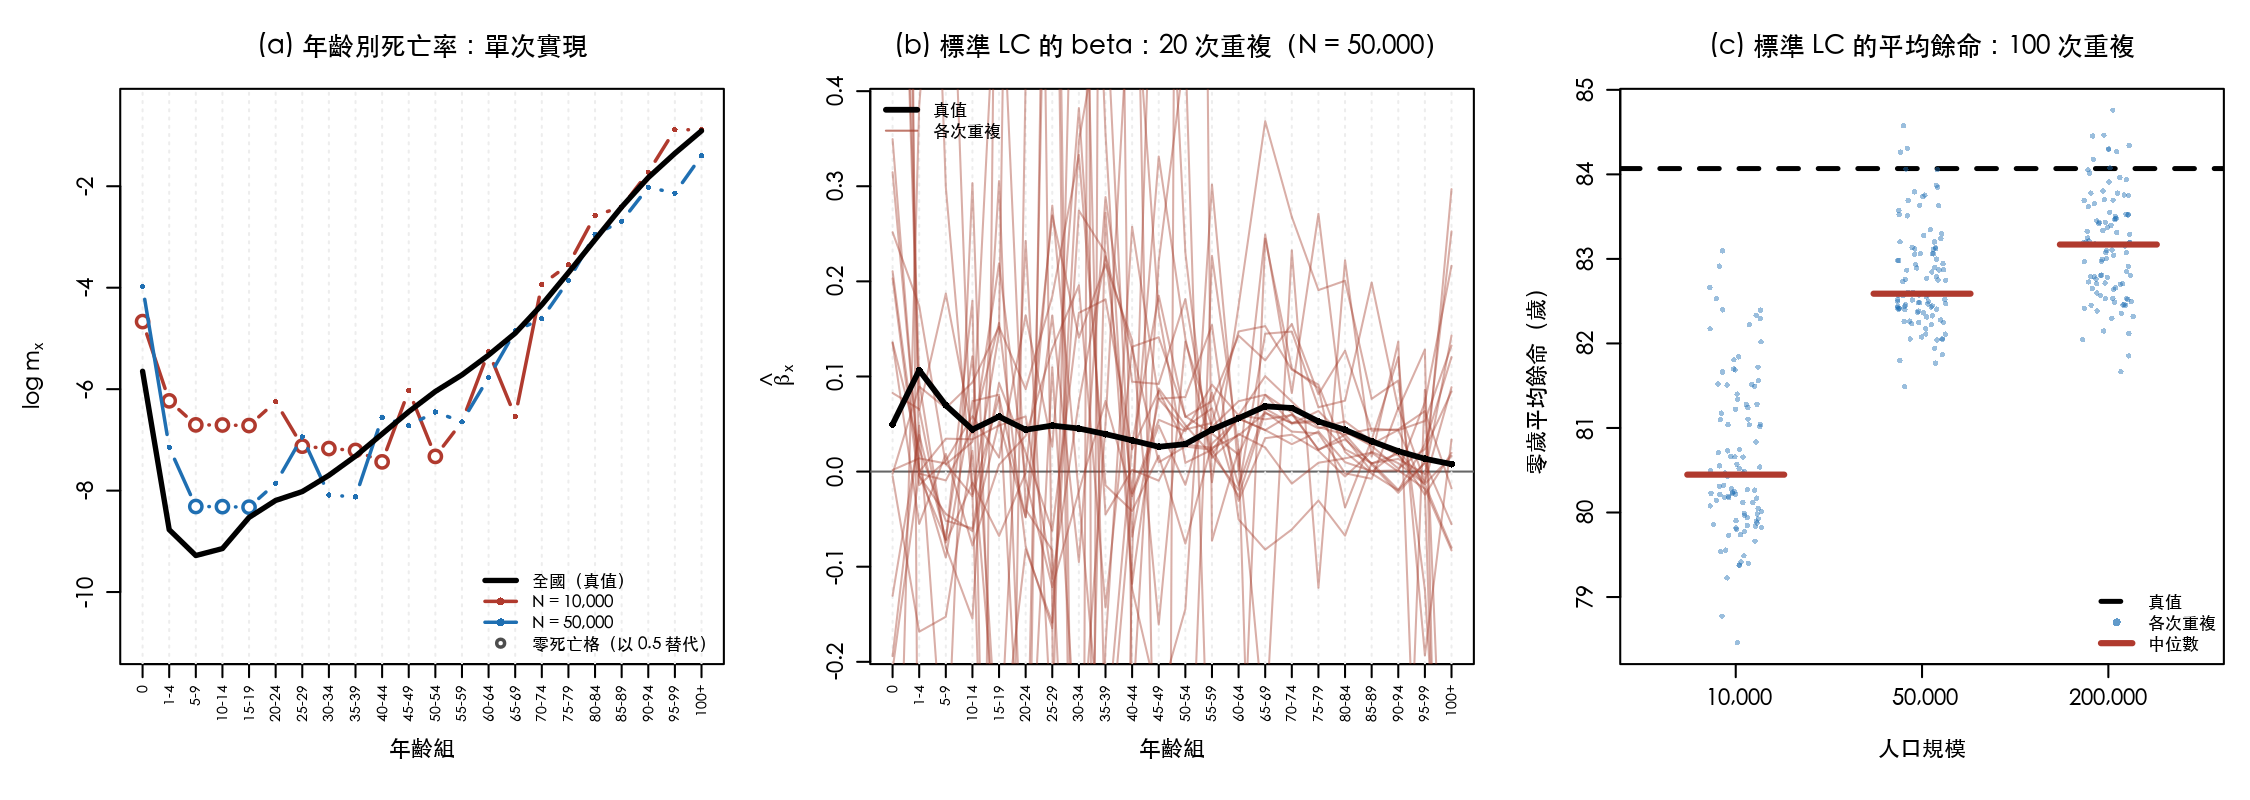
\includegraphics[width=\textwidth]{figT0_oscillation.png}
\caption{小人口下 LC 估計的震盪與偏誤（臺灣女性，以全國配適為真值）。
(a) 單次實現的年齡別死亡率：小人口的曲線劇烈跳動，而空心點為零死亡格，
其被替代後的位置\textbf{系統性地高於}真值曲線。
(b) $\hat\beta_x$ 的 20 次重複：形狀完全不穩定。
(c) 零歲平均餘命的 100 次重複：點雲全部落在真值（虛線）之下。}
\label{fig:osc}
\end{figure}

圖~\ref{fig:osc}(a) 顯示震盪的來源。人數一萬時 1 至 19 歲的各組幾乎全是
零死亡格（空心點），以 $0.5$ 替代後被擺在真值曲線之上約兩個對數單位；
人數五萬時情況緩解但仍有多格為零。值得注意的是這些點\textbf{不是隨機地
散在真值兩側}，而是一致偏高——震盪與偏誤在此是同一個機制的兩面。

圖~\ref{fig:osc}(b) 顯示震盪傳到參數上的結果。$\hat\beta_x$ 描述各年齡對
時間趨勢的敏感度，其真值（黑線）在幼年與 65 至 74 歲有兩個峰；
但 20 次重複的軌跡完全看不出這個形狀，甚至頻繁出現負值。

圖~\ref{fig:osc}(c) 則顯示兩個問題在標的量上同時出現，而且量級相當。
以配適末年的零歲平均餘命為例，真值為 $84.07$ 歲，而標準 LC 的重複中位數
在人數一萬、五萬、二十萬時分別為 $80.45$、$82.59$、$83.17$ 歲，
即系統性低估 $3.62$、$1.48$、$0.90$ 歲；同時 $5$ 至 $95$ 百分位的全距為
$3.00$、$1.84$、$2.01$ 歲。\textbf{人數五萬時偏誤（$1.48$ 歲）與整個隨機
全距（$1.84$ 歲）幾乎相同}，亦即把估計重複一百次所看到的全部變動，
其幅度不過與一個看不見的系統性偏移相當。考慮到我國縣市之間平均餘命的最大
差距約為 $10$ 歲，$1.48$ 歲的偏誤已足以使一個地區在排序上錯置數個名次。
換言之，若不處理偏誤，鄉鎮市區生命表所呈現的地區差異將有相當部分是估計
方法的產物而非真實的健康差異。

\subsection{小樣本估計的兩條傳統}

上一小節的兩個問題在統計學上各有其傳統，本文的取徑須放在這個脈絡中才能定位。
就小樣本估計而言，文獻的關注集中在偏誤（bias）與震盪（oscillation）兩個主題；
前者探討估計量的期望與真值之間的系統性落差，後者探討估計量在重複抽樣下的
變異。本小節先說明偏誤一支的發展，再說明震盪一支，兩者在第\ref{sec:lit}
會合於同一個估計方程的框架。

就 LC 模型而言，偏誤的具體表現已由既有文獻刻畫。Wang et al.（2018）以蒙地卡羅
模擬指出，當人口規模下降時 $\hat\alpha_x$ 與 $\hat\beta_x$ 會朝同一方向偏移，
在二十萬人以下時尤其明顯；Yue et al.（2019, Figure 1）進一步分離兩者，
指出 $\hat\alpha_x$ 的偏誤恆為正且量級遠大於 $\hat\beta_x$，
而後者在人數超過十萬時平均而言已接近零。余清祥等（2021）在臺灣鄉鎮市區的
實證中得到一致的結論。三篇研究共同指出的事實是：
$\hat\alpha_x$ 的偏誤有確定的方向，而 $\hat\beta_x$ 的偏誤沒有。
本文的推導即由此一事實出發，並在第\ref{sec:method}說明其成因與量級皆可解析求得。

小樣本的估計誤差可能來自數個不同的環節，釐清來源是設計修正方法的前提。
第一個環節是\textbf{分配假設}：死亡數通常設為 Poisson 分配，若真實的死亡過程
有過度離散（overdispersion），則以 Poisson 計算的變異數偏小，連帶影響加權與推論
（Delwarde et al. 2007）。第二個環節是\textbf{概似基礎統計量的高階項}：
即使分配假設正確，最大概似估計量在有限樣本下仍有 $O(n^{-1})$ 的偏誤，
而概似比統計量的分布也與其漸近的卡方分布有 $O(n^{-1})$ 的落差，
後者可由 Bartlett（1937）的乘數修正吸收。第三個環節是\textbf{非線性轉換}：
LC 的反應變數是 $\log(D/E)$ 而非 $D$ 本身，而取對數之後的期望不等於期望之後
取對數；在計量經濟學中這一點早有討論，Duan（1983）與 Santos Silva and
Tenreyro（2006）都指出對數轉換會使估計量系統性偏移，而其方向依賴誤差的分布。
第四個環節是\textbf{估計量本身的設定}，包括損失函數的形狀、觀測的權重、
以及是否加入懲罰。第五個環節則是\textbf{資料本身的變異}，即人數少所造成的
抽樣變異，這一項不是偏誤而是變異數，必須與前四項分開處理。
本文處理的是第三個環節，而第\ref{sec:method}將說明，LC 的零格替代使這一項
不只是漸近的高階項，而是一個不隨年數增加而消失的量。

處理偏誤的傳統自此分為兩支。第一支是\textbf{事後修正}：先取得最大概似估計值，
再扣除其偏誤的估計。Bartlett（1953）與 Cox and Snell（1968）給出該項的一般
展開式，Cordeiro and McCullagh（1991）把它寫成廣義線性模型中可由加權最小平方
一次求得的形式。此支的優點是目標明確，缺點則是它\textbf{須建立在最大概似
估計值存在且有限的假設上}；若該假設不成立，事後修正無從施加。
第二支即為因應此一限制而生的\textbf{預先修正}：Firth（1993）指出，
把偏誤的首項移到分數函數上，等價於在概似上乘一個 Jeffreys 型的懲罰，
如此估計值恆為有限，且不需要先有最大概似估計值。
Kosmidis and Firth（2009）把該作法推廣到指數族非線性模型，
使其適用範圍涵蓋 LC 這類雙線性的設定。兩支的共同限制是修正的量隨模型而異，
目前並無涵蓋所有模型的通用公式；Cordeiro and McCullagh（1991）在其結語中
即以此說明為何每一類模型都須個別推導。

處理震盪的傳統則有兩條平行的發展。第一條是 $M$-估計。
Huber（1964）把最大概似推廣為「某個估計方程的解」，其作法是在殘差超過某個
門檻之後把損失函數由二次式改為一次式，使少數離群觀測的影響有界；
Hampel（1974）的影響函數與 Donoho and Huber（1983）的崩潰點則分別刻畫
單一觀測的影響力與可承受的污染比例上限。$M$-估計的優點是把估計量的性質
化約為估計方程的期望與變異數兩件事，因而可以在不完全指定分布的情形下給出
保證；其代價是效率，因為為了在未知的污染下仍然可靠，必須放棄一部分在模型
正確時本可獲得的精度（Huber and Ronchetti 2009, 第 1 章）。
這個代價是否值得，取決於污染比例是否真的未知。

第二條是正則化。Hoerl and Kennard（1970）的 Ridge 與 Tibshirani（1996）的
LASSO 以在目標函數上加懲罰項的方式，以少量偏誤換取變異數的降低，
其正當性可追溯至 Stein（1956）的不可容許性與 James and Stein（1961）的
收縮估計；在小區域估計中，Fay and Herriot（1979）的經驗貝氏收縮是同一想法
的區域層級版本。正則化的代價是須指定懲罰強度，而該強度通常以交叉驗證選出。

在死亡率文獻中，上述兩條傳統又各自有以\textbf{參考母體}為工具的版本。
Lee（2003）的 partial SMR 修勻以標準化死亡比為中心，把小區域的年齡別死亡率
朝人數較多的參考母體收縮，收縮的權重由兩個母體之間的異質性估計值決定；
Li and Lee（2005）的 coherent LC 則合併多個母體的資料以降低估計誤差。
Yue et al.（2019）把 partial SMR 與 Whittaker（1923）修勻接在 LC 之前或之後，
以模擬比較兩種接法在七種死亡率比值情境下的表現，發現當小區域與參考母體
的年齡別死亡率成固定比例時 partial SMR 明顯最佳，但當兩者型態不同時
其誤差反而大於不修勻的情形。這一條線與本文的關係最為直接，
第\ref{sec:result}之五將以同一組模擬設計與本文的修正並列比較。

\subsection{小樣本 $M$-估計的理論發展與應用}

上述兩條傳統在近二十年逐漸合流，而合流處正是本文所需的工具。
值得先指出的是，把偏誤修正與 $M$-估計接在一起並非本文首創。
Firth（1993）本人即把其預先修正定義在一般的估計方程上，而非僅限於概似；
Kosmidis and Firth（2009）進一步把修正寫成對估計方程加一個可計算的位移項，
其形式與本文所採的中心化完全同類。此一先例的優點在於：
修正施加在估計方程而非估計值上，因而不需要估計值先存在，
也不需要目標函數是某個概似——這兩項性質正是本文所需要的，
因為零格的存在使 LC 的 Poisson 最大概似可能不存在（Albert and Anderson 1984），
而標準 LC 的目標函數本就不是任何分配的對數概似。

在理論上，$M$-估計的框架被推廣到三個方向。其一是與分位數的合併：
Breckling and Chambers（1988）把 Huber 的損失乘上一個依殘差正負而異的
非對稱權重，得到由穩健程度與非對稱度兩個參數索引的 M-分位數族，
其兩個極限分別是 Koenker and Bassett（1978）的檢查函數與
Newey and Powell（1987）的非對稱最小平方。其二是與懲罰的合併：
Zoubir et al.（2018，第 3 章）整理了穩健損失與 Lasso／Elastic Net 的結合，
並給出迴歸係數與尺度的聯合懲罰式 $M$-估計；Hu et al.（2021）則處理高維情形下
的漸近理論。其三是與相依資料的合併：Liang and Zeger（1986）的廣義估計方程
以工作相關矩陣處理相依而不指定聯合分布，Merlo et al.（2022）進一步把它推廣到
帶 Huber 損失的 M-分位數。

在應用上，這條線在小區域估計中發展得最完整。
Chambers and Tzavidis（2006）以 M-分位數取代 Fay--Herriot 的隨機效果假設，
理由是前者可直接給出各區域自己的係數而不必假設區域效果的分布；
Bianchi et al.（2018）補上推論理論，Ranalli et al.（2023）加入 Lasso 與
Elastic Net 懲罰並應用於空氣品質，Dawber et al.（2022）處理離散標的，
Bugallo et al.（2026）則針對均方誤差估計提出偏誤校正；
Lahiri and Salvati（2023）把巢式誤差迴歸推廣到同時容許區域別係數與區域別
變異成分的情形。這些工作的應用場景多為家戶調查的地方層級指標估計，
其共同特徵是以較弱的分布假設換取穩健性，而其漸近理論均假設解釋變數已觀測。
本文的情形與此有一處重要差異：LC 的 $\kappa_t$ 是待估的潛在變數而非觀測值，
因此上述理論不能直接套用，這一點將在第\ref{sec:disc}列為限制。

\subsection{既有方法在本問題上的適用性}

綜合上述研究與實證可以得到三項判斷，而這三項判斷決定了本文的設計。

第一項判斷是：正則化一脈的方法在本問題上失去其標準的選參程序。
懲罰強度通常以交叉驗證選出，而交叉驗證要求觀測可以切分為訓練與驗證兩部分；
但 LC 的識別完全依賴年齡與年份兩個方向的跨格借力，任何對年齡--年份格的切分
都會破壞其秩一雙線性結構，使被留置的格無法由其餘的格預測。
Ranalli et al.（2023）與 Hu et al.（2021）的懲罰式 M-分位數都需要選定
$\lambda$，其論文中的選參程序即建立在觀測可自由切分的前提上，
此一前提在本問題並不成立。

第二項判斷是：$M$-估計的效率代價在此不必支付。
穩健方法之所以犧牲效率，是因為污染比例 $\varepsilon$ 未知，必須針對最壞的情形設計
（Huber 1964）。但本文第\ref{sec:method}之三將指出，小人口 LC 的「污染」
並非來自外部的離群值，而是來自零格替代這個分析步驟，其比例恰為 Poisson 的
零機率 $e^{-\mu}$，拿到曝露數與配適值即可計算。
既然污染比例已知，便不必為未知的最壞情形預留餘裕，而可直接計算其後果並扣除。

第三項判斷是：$M$-估計真正可借用的不是穩健性，而是更基本的一項性質。
$M$-估計理論要求估計方程在真值處的期望為零，即 Fisher 一致性。
這個條件在教科書中通常一行帶過，因為在其標準設定下它自動成立；
但它自動成立的前提是損失函數作用在未經轉換的反應變數上
（Huber and Ronchetti 2009, 第 3 章）。標準 LC 先取對數又替代零格，
兩者都是非線性運算，該條件因而不再自動成立。
本文的切入點即在於此：把既有研究以模擬觀察到的偏誤，
放回 $M$-估計理論中它本來的位置，並說明該估計量在零死亡格上的行為
如何能在不過度犧牲效率的前提下加以修正。

\subsection{研究設計}

基於上述，本文設計一個 LC 的修正估計，其推導依序借用三篇脈絡的性質。

由 \textbf{Huber（1964）} 的 $M$-估計框架，本文把標準 LC 辨識為取平方損失的
$M$-估計量，並依 Fisher 一致性的要求計算其估計方程在真值處的期望；
該期望不為零，其量有閉式，而 $M$-估計對此的標準補救是中心化估計方程。
所提的修正因此不是另行發明，而是這個標準補救在本問題的具體形式。

由\textbf{混合模型}的表示法（McLachlan and Peel 2000；Yao and Xiang 2024），
本文說明零格替代在統計上是什麼：它使每一格成為一個兩成分混合，
而混合權重已知。此一表示同時給出中位數類估計量失效的解析門檻，
並釐清本文的情形與 Lambert（1992）的零膨脹模型有何不同。

由 \textbf{M-分位數與懲罰}的一般目標函數（Breckling and Chambers 1988；
Zoubir et al. 2018；Ranalli et al. 2023），本文說明標準 LC 是該式的一個角落，
而小人口的各種既有補救各自改動了其中一項設定；
據此可判斷本文的修正與它們的關係是正交的，並導出兩項可事先檢驗的預測。

在死亡率文獻中，與本文最接近的是 Yue et al.（2019）。該文以修勻修改 LC 在
小人口的估計，其修勻的資訊來自一個人數較多的參考母體。兩者的差別有二。
其一是處理的對象：修勻降低的是觀測的變異，屬處理震盪的一路；
本文的修正改變的是估計方程的中心，屬處理偏誤的一路。
其二是所需的外部資訊：partial SMR 與 Whittaker 修勻都要求存在一個與目標
小區域死亡率型態相近的參考母體，而該文自己的模擬即顯示，當兩者的年齡別
死亡率型態不同時 partial SMR 的誤差會明顯惡化；本文的修正只用到目標區域
自己的曝露數與配適值，不需要參考母體，但代價是它依賴 Poisson 假設。
兩者因此是以不同的外部資訊換取穩定，而不是同一件事的兩種作法。
第\ref{sec:result}之五將以 Yue et al.（2019, Figure 2）的七種死亡率比值情境
把兩者並列比較，以回答「何時該用參考母體、何時該用分配假設」這個問題。

本文因此在實證上安排五項檢驗，依序回答五個問題：
閉式能否預測實測偏誤（第\ref{sec:valid}之二）；
偏誤是否隨人口年齡結構而變、閉式能否一併解釋（第\ref{sec:valid}之三）；
修正後的估計量與既有作法相比如何（第\ref{sec:result}之二）；
改善集中在哪些年齡（第\ref{sec:result}之三）；
以及修正是否以變異數為代價（第\ref{sec:result}之四）。
最後以參考母體修勻（第\ref{sec:result}之五）與真實資料抽薄
（第\ref{sec:result}之六）兩項外部檢驗收尾。

\section{文獻回顧}\label{sec:lit}

本節回顧三條脈絡。三者並非死亡率文獻，而是本文推導所依的一般統計理論；
回顧的重點因此放在\textbf{各條脈絡的核心性質}，以及\textbf{該性質在其原始
應用場景與本文情境之間的落差}。第\ref{sec:method}再由這些性質往下推到 LC。

\subsection{$M$-估計與 Fisher 一致性}

Huber（1964）提出 $M$-估計量，把最大概似的想法推廣為「某個目標函數的
極小值」或等價地「某個估計方程的解」：$\hat\theta$ 解
$\sum_i\psi(y_i;\theta)=0$，其中 $\psi$ 不必是對數概似的導數。
該文的動機是位置參數的穩健估計，設定為 $\varepsilon$-污染——絕大多數觀測
來自模型、少數來自別處——目標是使少數觀測無法主導估計。
Hampel（1974）以影響函數刻畫單一觀測的影響力，
Donoho and Huber（1983）以崩潰點刻畫可承受的污染比例上限，
Huber and Ronchetti（2009）為該領域的標準專著。
在應用上，$M$-估計已是訊號處理、電力系統狀態估計與電腦視覺的常規工具
（Zoubir et al. 2018），其場景的共同特徵是觀測數遠大於參數數、
且離群值確實是少數。

$M$-估計的另一條發展線把「估計方程」本身當成建模的對象，而不必先寫下
概似。Godambe 的估計函數理論與 Liang and Zeger（1986）的廣義估計方程
即屬此類，後者以工作相關矩陣處理相依資料而不指定聯合分布，
在縱貫資料分析中已成常規；Merlo et al.（2022）進一步把廣義估計方程推廣到
帶 Huber 損失的 M-分位數。這條線對本文的意義是它確立了一個看法：
一個估計量的性質，可以完全由其估計方程的期望與變異數讀出，
而不必訴諸該估計量是否為某個概似的最大值。本文正是循此讀 LC。

本文所需的性質不是穩健性，而是 $M$-估計理論中更基本的一項：
\textbf{Fisher 一致性}。一個 $M$-估計量要在真值 $\theta_0$ 處一致，
必要條件是估計方程在真值處的期望為零，
$\Ex_{\theta_0}[\psi(Y;\theta_0)]=0$；否則 $\hat\theta$ 收斂到的是
使該期望為零的另一個點，與 $\theta_0$ 相差一個不隨樣本數消失的量。
此一條件在教科書中通常一行帶過，因為對最大概似而言它自動成立
（分數函數的期望為零），對最小平方而言只要誤差期望為零即成立。
但它之所以自動成立，前提是損失函數作用在未經轉換的反應變數上。
一旦反應變數先經過非線性轉換，$\Ex[\psi]=0$ 就不再是自動的——
這正是本文的切入點。

與本文情境的落差因此有三。其一，古典 $M$-估計文獻關心的是
$\psi$ 有界所帶來的穩健性，而本文關心的是 $\psi$ 的\textbf{期望}是否為零，
兩者是不同的問題：平方損失的 $\psi(u)=u$ 完全不穩健，
但若 $\Ex[u]=0$ 它仍是一致的；反之一個很穩健的 $\psi$ 若 $\Ex[\psi]\ne0$
則仍不一致。古典文獻少談後者，因為在其標準設定（損失作用在原始反應變數上）
中它自動成立。其二，古典設定的觀測數遠大於參數數，而 LC 模型每個
$\alpha_x$ 只有 $T$ 個觀測（本文 $T=24$），每個 $\kappa_t$ 只有 $A$ 個
（本文 $A=22$）。其三，古典設定的污染比例未知，而本文的情形不然
（見下一小節）。

還有一項結構上的落差值得先點出。古典 $M$-估計的參數進入模型的方式是線性的
（$x_i^{\top}\theta$），而 LC 的 $\alpha_x+\beta_x\kappa_t$ 對
$(\beta,\kappa)$ 是\textbf{雙線性}的，識別須靠式~\eqref{eq:lc} 的兩個約束。
這使 $\hat\beta$ 與 $\hat\kappa$ 的漸近理論複雜得多。
所幸本文所處理的 $\hat\alpha_x$ 不受此影響——它在雙線性部分被估計之前
即已由列平均定出，因此可以完全在單變數 $M$-估計的框架內分析。
這也是本文把範圍限於 $\alpha_x$ 的技術理由。

\subsection{混合模型與污染比例}

有限混合模型把觀測的分布寫成若干成分分布的加權和，
$f(y)=\sum_{j}\pi_j f_j(y)$。其發展脈絡自 Pearson（1894）以動差法分解
螃蟹前額寬的雙峰分布起，長期受限於計算；
Dempster et al.（1977）的 EM 演算法使最大概似估計成為可行，
此後混合模型成為模型式分群的標準工具，McLachlan and Peel（2000）與
Yao and Xiang（2024）為前後兩代專著，後者涵蓋半參數推廣、穩健建模、
標籤交換與高維情形。在應用上，混合模型用於天文、基因體、經濟與金融等
領域的異質資料；在小區域估計中，Del Sarto et al.（2019）以 M-分位數迴歸的
有限混合處理未觀測異質性，De Nicol\`o et al.（2023）以 Beta 混合估計地區的
不均度指標。

與計數資料最相關的一支是零膨脹模型。Lambert（1992）的零膨脹 Poisson 迴歸把
觀測寫成「一個零處的點質量」與「一個 Poisson 」的兩成分混合，用以處理
製造業瑕疵計數中零的個數遠多於 Poisson 所能解釋者。其形式與本文
第\ref{sec:method}將導出的式~\eqref{eq:mix} 極為相似，因此須把差別講清楚，
否則容易誤讀。零膨脹模型所處理的是\textbf{結構上多出來的零}——
亦即資料生成機制本身含有一個「必然為零」的狀態，故零的個數超過 Poisson
的預期。本文的情形\textbf{不是}零膨脹：死亡數就是純粹的 Poisson ，
零的個數恰如 $e^{-\mu}$ 所預期，沒有任何多餘。本文的混合是
替代規則在取對數之後的變數上造出來的——因為 $\log 0=-\infty$
不可用，分析者必須把所有零格對應到同一個值 $\log(c_0/E)$，
於是轉換後的變數才出現一個點質量。換言之，零膨脹模型的混合來自
\textbf{資料}，本文的混合來自\textbf{分析步驟}。這個差別有實質後果：
零膨脹模型須估計膨脹比例，而本文的混合權重由 Poisson 本身給定，
無須估計；反之零膨脹模型可以不取對數而直接配適，本文的困難則完全來自
取對數這個步驟。

混合模型與穩健統計的連結早已建立：Huber 的 $\varepsilon$-污染模型
$(1-\varepsilon)F+\varepsilon H$ 就是一個兩成分混合。但兩個文獻的處理方式
相反。混合模型把 $\pi_j$ 與 $f_j$ 都當成待估的參數，以 EM 求解；
穩健統計則把 $\varepsilon$ 與 $H$ 當成未知的滋擾，設計對其不敏感的估計量。
穩健估計量之所以必須付出效率代價，正是因為 $\varepsilon$ 未知：
它必須針對最壞的情形設計。

與本文情境的落差正在此處，而這個落差對本文有利。
第\ref{sec:method}將指出，零格替代使每一格的觀測成為一個兩成分混合，
而其混合權重是\textbf{已知的}——它就是 Poisson 的零機率 $e^{-\mu}$，
拿到資料即可估計。既然如此，既不必以 EM 去估它，也不必為不知道它而
承擔該項效率損失。另一項落差則不利：該混合的其中一個成分是\textbf{退化的}
（一個點質量），而有限混合理論通常假設各成分有密度，
故識別性、標籤交換等標準議題在此不適用，EM 亦無從施加。

\subsection{M-分位數與懲罰式估計}

第三條脈絡把損失函數、權重與懲罰整合為一個目標函數。
Koenker and Bassett（1978）以檢查函數 $\rho_\tau$ 取代平方損失，
使迴歸得以刻畫條件分位數；Koenker（2005）為標準參考，
其應用場景包括勞動經濟學的薪資分布與兒童生長參考曲線
（Wei et al. 2006），共同特徵是每個共變數水準上有大量觀測。
Breckling and Chambers（1988）指出，若把 Huber 損失乘上一個依殘差正負
而異的非對稱權重，即得一個由 $(\tau,c)$ 索引的損失函數族 M-分位數，
其兩個極限分別是檢查函數（$c\to0$）與非對稱最小平方
（$c\to\infty$，Newey and Powell 1987）。
Chambers and Tzavidis（2006）把 M-分位數帶進小區域估計，
Bianchi et al.（2018）補上推論理論。

M-分位數之所以在小區域估計中受青睞，理由值得一提，因為它與本文的
取捨相關。傳統的小區域估計以 Fay and Herriot（1979）的隨機效果模型為主，
須假設區域效果的分布（通常為常態）；Chambers and Tzavidis（2006）指出
M-分位數可直接給出各區域自己的迴歸係數而不必作此假設，
因而對分布誤設較不敏感。其應用多為家戶調查資料的地方層級所得與剝奪指標
估計，Bianchi et al.（2018）另處理了推論，Bugallo et al.（2026）則針對
均方誤差估計提出偏誤校正。這一脈的共同特徵是\textbf{以較弱的分布假設
換取穩健性}。本文的取向相反：本文明確採用 Poisson 假設，
並以此換取一個可完全算出的偏誤。兩者各有代價——若 Poisson 假設不成立，
本文的校正就失去依據（見第\ref{sec:disc}）；而若分布假設其實成立，
放棄它就等於放棄可用的資訊。

再加上懲罰即得本文所需的完整形式。Zoubir et al.（2018，第 3 章）
整理了穩健損失與 Lasso／Elastic Net 的結合，包含迴歸係數與尺度的聯合
懲罰式 $M$-估計；Ranalli et al.（2023）以 Lasso 與 Elastic Net 懲罰的
M-分位數迴歸分析交通與氣象對空氣品質的影響；
Hu et al.（2021）另以損失的冪次為刻度提出 $L_p$-分位數並處理高維懲罰。
綜合之，這條脈絡的一般目標函數為
\begin{equation}\label{eq:general}
\min_{\theta}\ \sum_{i} w_i\,\rho_{\tau,c}(u_i(\theta))\;+\;\lambda P(\theta),
\end{equation}
其中含三項設定：損失形狀 $(\tau,c)$、權重 $w$、懲罰 $(\lambda,P)$。

與本文情境的落差有二。其一，這條脈絡的應用場景是單位層級的調查資料，
每個小區域有多個受訪單位；而死亡率資料是聚合的計數，每格只有一個觀測。
其二，三項設定都需要調參（$\tau$、$c$、$\lambda$），
而本問題既無真值、亦無法以交叉驗證選參——切分年齡--年份格會破壞
雙線性結構所依賴的跨格借力。本文因此不使用這條脈絡的方法，
而是借用它的\textbf{分類}：式~\eqref{eq:general} 把標準 LC 納為一個角落
（$\tau=0.5$、$c=\infty$、$w\equiv1$、$\lambda=0$），
因而可以用來判斷各種補救各自動了哪一個設定，以及本文的校正動的是什麼。

\subsection{參考母體修勻：以外部資訊換取穩定}\label{sec:ref}

前三條脈絡都只使用目標母體自己的資料。死亡率文獻另有一條不同的路徑，
其作法是引入一個人數較多的參考母體，以外部資訊壓抑小區域的震盪。
由於第\ref{sec:result}之五要與這條路直接比較，此處須把它的性質寫清楚。

Lee（2003）提出的 partial SMR 修勻以標準化死亡比為中心。
記 $d_x$ 為目標小區域 $x$ 歲組的死亡數觀測值、$P_x$ 為其曝露數、
$m^R_x$ 為參考母體同年齡組的中央死亡率，則期望死亡數為 $e_x=P_x m^R_x$，
標準化死亡比為 $\mathrm{SMR}=\sum_x d_x\big/\sum_x e_x$。
修勻後的死亡率定義為
\begin{equation}\label{eq:psmr}
v_x \;=\; m^R_x\,\exp\!\left(
\frac{d_x\hat h^2\log(d_x/e_x)+\bigl(1-d_x/\textstyle\sum_x d_x\bigr)\log \mathrm{SMR}}
     {d_x\hat h^2+\bigl(1-d_x/\textstyle\sum_x d_x\bigr)}\right),
\end{equation}
其中 $\hat h^2=\max\bigl\{[\sum_x(d_x-e_x\mathrm{SMR})^2-\sum_x d_x]
\big/[\mathrm{SMR}^2\sum_x e_x^2],\,0\bigr\}$ 度量兩個母體之間年齡別死亡率
型態的異質性。式~\eqref{eq:psmr} 是觀測的對數死亡比 $\log(d_x/e_x)$ 與整體
$\log\mathrm{SMR}$ 的加權平均，其權重的設計使死亡數愈少的年齡愈倚賴參考母體。
此一形式與保險的信賴度估計同型（Klugman et al. 2012），
也與 Kimeldorf and Jones（1967）的貝氏修勻同屬一類。

對本文而言，式~\eqref{eq:psmr} 有兩項性質最為關鍵。
第一，$d_x=0$ 時第一項的權重為零，修勻值退化為 $\mathrm{SMR}\cdot m^R_x$，
恆為正。參考母體修勻因此根本不需要 $c_0$ 之類的替代值，
零格的困難在這條路上是以外部資訊解決的，而非以慣例解決的。
第二，$\hat h^2=0$ 時所有年齡都完全採用 $\mathrm{SMR}\cdot m^R_x$，
亦即整條年齡曲線的\textbf{形狀}來自參考母體，只有水準由目標區域決定。
這說明該法的表現必然取決於兩個母體的形狀是否相近。

Yue et al.（2019）正是以此為主題。該文另考慮 Whittaker（1923）修勻的比值版本，
即先取 $s_x=(d_x/P_x)/m^R_x$，再以
$\min_r \sum_x w_x(r_x-s_x)^2+h\sum_x(\Delta^z r_x)^2$ 求修勻後的比值，
取 $w_x$ 為曝露數、$h$ 為各年齡曝露數的平均。
該文設計七種比值情境（$s_x$ 固定為 $0.8$、$1.0$、$1.2$，以及隨年齡遞增、
遞減、V 型、倒 V 型），以 100,000 人對 2,000,000 人的模擬比較，
結論是：在前三種情境下 partial SMR 的平均絕對百分比誤差明顯最小
（約 $12\%$，不修勻為 $25$--$29\%$），但在「遞增」情境下惡化至 $47.65\%$，
反而遠劣於不修勻；Whittaker 比值修勻則在七種情境下都穩定在 $14$--$19\%$。
該文並指出，若把遞增情境的比值範圍由 $0.5$--$1.5$ 縮為 $(1-a)$--$(1+a)$，
則 $a\le 0.4$ 時 partial SMR 仍較佳。

這條脈絡與本文情境的落差，與前三條脈絡的落差性質不同。
前三條的落差在於理論前提（污染比例未知、觀測可切分、成分有密度），
這一條的落差則在於\textbf{資料的可得性}：
它要求分析者先有一個型態相近的參考母體，而在鄉鎮市區的應用中，
自然的參考母體是全國或鄰近地區，但臺灣縣市之間零歲平均餘命的最大差距
超過十歲（Yue et al. 2019），鄰近地區的社經組成亦常有明顯差異
（Wang and Yue 2026）。換言之，這條路把問題由「如何從少量資料估計」
轉為「如何判斷參考母體是否可用」，而後者本身即是一個未解的問題。
本文的修正不需要參考母體，但須假設 Poisson ；
兩者因此是兩種不同的外部資訊，第\ref{sec:result}之五以模擬量化其取捨。

\subsection{三條脈絡的核心性質與其在本問題上的落差}

把前四小節收束起來，本文所借用的性質與其落差可以一併陳述。

由 $M$-估計，本文借用的是 Fisher 一致性這一必要條件：
$\Ex[\psi]=0$ 為估計量在真值處一致的必要條件（Huber 1964）。
該條脈絡的原始應用場景是位置參數與迴歸係數的穩健估計，
近年則以訊號處理與電力系統狀態估計為大宗（Zoubir et al. 2018），
其共同特徵是觀測數遠大於參數數、且離群值確實是少數。
本文的情境兩項皆不成立：每個 $\alpha_x$ 只有 $T$ 個觀測，
而幼年組的零格比例可達七成以上。但所借用的性質不受此影響，
因為 Fisher 一致性是對估計方程期望的陳述，與觀測數無關。
第\ref{sec:method}之二將指出標準 LC 是取平方損失的 $M$-估計量，
其 $\Ex[\psi]=b(\mu;c_0)\neq0$，故 Fisher 不一致，
而 $M$-估計對此的標準補救即為中心化估計方程。

由混合模型，本文借用的是 $\varepsilon$-污染即兩成分混合這一表示，
以及中位數崩潰點為 $50\%$ 這一結果（Donoho and Huber 1983）。
該條脈絡的原始應用場景是模型式分群、零膨脹計數（Lambert 1992）
與小區域的未觀測異質性（Del Sarto et al. 2019），
其共同設定是混合權重未知而待估。本文的落差在於混合權重\textbf{已知}，
且其中一個成分是退化的點質量；前者對本文有利，後者則使 EM 無從施加。
第\ref{sec:method}之三將由此得到中位數失效的解析門檻 $\mu<\ln 2$。

由 M-分位數與懲罰，本文借用的不是方法而是\textbf{分類}：
式~\eqref{eq:general} 以損失形狀、權重、懲罰三項設定涵蓋一大類估計量，
而標準 LC 是其中 $\tau=0.5$、$c=\infty$、$w\equiv1$、$\lambda=0$ 的角落。
該條脈絡的原始應用場景是家戶調查的小區域指標估計與高維變數選擇，
其三項設定都需要調參，而調參程序建立在觀測可自由切分的前提上。
本文不使用該脈絡的方法，但以其分類判斷：
三項設定皆不改變 $\Ex[\psi]$，故本文的偏誤校正與三者正交。

\subsection{既有方法所載的限制，以及本文檢驗它們的位置}\label{sec:limtable}

上述每一項工具，其原始文獻都同時記載了優點與限制。
本文的實證部分並非另起爐灶地比較各種方法的優劣，而是逐項檢驗這些已被
記載的限制在小人口 LC 上是否確實出現、以及出現時的量級。
以下依序說明七項限制與本文檢驗它們的位置，後續各節的每一項結果都可回到
其中一項，第\ref{sec:disc}將逐項回顧。

事後修正的優點是目標明確，直接扣除 $O(n^{-1})$ 的偏誤項；
其限制則是必須先有有限的最大概似估計值，Firth（1993）在導論中即明言此點。
本文第\ref{sec:result}之二顯示，人數一萬時 Poisson 最大概似的 $\alpha$ 最大偏誤
達 $13.03$，該前提確實不成立；本文改由 $D$ 的邊際分布推導偏誤，
不需要最大概似估計值先存在，因而繞過此一限制。

預先修正的優點正是在最大概似不存在時仍可施加，其限制則是它所修正的是
$O(n^{-1})$ 的漸近項，且仍須寫得出概似。
本文第\ref{sec:result}之二顯示，人數一萬時 Firth 的 $\alpha$ 最大偏誤仍有
$0.43$ 而非零，與「只修正首項」的性質相符；
但相對於未修正的 $13.03$ 已是決定性的改善。

穩健損失的優點是不需知道污染的分布即可提供保障，其限制有二：
效率代價（中位數在常態下的相對效率僅 $2/\pi\approx0.64$，
Huber and Ronchetti 2009）與「污染為少數」的前提。
本文第\ref{sec:method}之三指出污染比例 $\pi=e^{-\mu}$ 為已知，
故效率代價不必支付；而幼年組的 $\pi$ 可達 $0.74$，
「少數」的前提在本問題並不成立。

崩潰點理論的優點是給出方法適用範圍的上界，其對中位數的上界為 $50\%$。
本文第\ref{sec:method}之三把該上界代入混合表示，得到解析門檻
$\mu<\ln 2=0.693$；$\mu=0.3$ 時 $\pi=0.741$，與實測的零格率相符。

正則化的優點是以少量偏誤換取大量變異數的降低，其限制是須指定懲罰強度，
而該強度通常以交叉驗證選出。本文第\ref{sec:lit}之三已說明該程序在此不可行；
第\ref{sec:result}之二則顯示資訊加權使 $\beta$ 的帶寬收窄約七倍卻使中線
略微偏離真值，正是「以偏誤換變異數」這個取捨的具體形式。

經驗貝氏收縮的優點是收縮量由變異成分決定而無須調參，
其限制是假設直接估計量不偏、僅有抽樣噪音。
本文第\ref{sec:betadec}的分解顯示 $\hat\beta_x$ 本身即有確定性的偏誤成分
（佔總誤差的 $9.2\%$），該前提因而不完全成立。

參考母體修勻的優點是直接降低觀測的震盪，且在零格上不需要替代值；
其限制是須有型態相近的參考母體，Yue et al.（2019）自己的模擬即顯示
型態不同時誤差反而惡化。本文第\ref{sec:result}之五以同一組情境檢驗此點，
並一併回答「若改以標準化死亡比填補零格，是否會得到與 $c_0=0.5$ 相同的結果」。

\subsection{本文後續的安排}\label{sec:roadmap}

依第\ref{sec:limtable}所列的檢驗清單，本文後續分四節進行，每一節回答一組
依序遞進的問題。

第\ref{sec:method}處理方法論與推導，回答「標準 LC 違反了哪一個條件、
違反的量是否有閉式」。該節先寫定記號與標準 LC 的兩階段估計流程，
再把標準 LC 辨識為取平方損失的 $M$-估計量，依 Fisher 一致性的要求計算其
估計方程在真值處的期望，得到閉式 $b(\mu;c_0)$，
並依 $M$-估計的標準補救導出修正的估計量；
接著以混合模型的表示法說明零格替代在統計上是什麼，
並由崩潰點理論導出中位數失效的解析門檻；
再以 M-分位數 LASSO 的一般目標函數說明該修正與既有補救的關係。
該節同時把 $\alpha_x$ 與 $\beta_x$ 的偏誤分解為確定性與隨機兩個成分，
這個分解決定了後續每一項結果的解讀方式；末一小節寫定全部模擬的設定。

第\ref{sec:valid}處理推導的驗證，回答兩個問題。
其一是閉式能否預測實測的逐年齡偏誤；此步驟的目的不是比較方法優劣，
而是確認推導本身正確，若閉式與實測不符，後續的修正即失去依據。
其二是偏誤是否隨人口的年齡結構而變；閉式對此給出一個可檢驗的預測，
因為年齡結構正是透過期望死亡數進入閉式的。

第\ref{sec:result}處理實證分析，回答「修正在臺灣資料上能改善多少、
以及改善不到的部分是什麼」。該節依序呈現整體指標的比較、
逐年齡的改善剖面、平均餘命的偏誤與離散、與參考母體修勻法的比較、
真實觀測死亡數抽薄下的穩健性檢驗，以及兩參數能否同時改善的分析。
每一項結果都對應第\ref{sec:limtable}所列的某一項限制。

第\ref{sec:disc}為結論、限制與後續工作，逐項回顧第\ref{sec:limtable}所列的
各項限制，說明哪些在本問題上確實出現、哪些因情境不同而得以繞過，
並列出本文推導尚未涵蓋的部分。

\section{研究方法}\label{sec:method}

\subsection{模型、記號與標準 LC 的估計}

本節先寫定記號與標準 LC 的估計流程，作為全文的基準。
本文以標準 LC 模型為基準模型（baseline），並以三類修正方法與之比較：
Firth（1993）的預先修正、本文由 $M$-估計導出的中心化修正，
以及 Lee（2003）與 Yue et al.（2019）的參考母體修勻。
由於本文全部的論證都建立在「標準 LC 的 $\hat\alpha_x$ 是如何定義的」
這一點上，以下的流程敘述力求與實作一致。

參照 Lee and Carter（1992），令 $x=1,2,\dots,A$ 為年齡組、
$t=1,2,\dots,T$ 為年份，LC 模型可以下式表達：
\begin{equation}\label{eq:lc}
\log m_{x,t}=\alpha_x+\beta_x\kappa_t,\qquad
\sum_x\beta_x=1,\quad \sum_t\kappa_t=0 .
\end{equation}
其中 $m_{x,t}$ 為 $x$ 歲組於 $t$ 年的中央死亡率；
$\alpha_x$ 為 $x$ 歲組的死亡水準，即該年齡組對數死亡率在觀測期間的平均；
$\beta_x$ 為 $x$ 歲組的年齡敏感度，刻畫該年齡組的對數死亡率對時間因子
變動一單位的反應幅度；$\kappa_t$ 為 $t$ 年的死亡改善因子，
刻畫全體年齡共同的時間趨勢。兩個約束用以固定參數的尺度與位置，
否則 $(\beta_x,\kappa_t)$ 可同乘與同除一個常數而不改變配適值。

觀測為死亡數 $D_{x,t}$ 與曝露數 $E_{x,t}$。本文設
\begin{equation}\label{eq:pois}
D_{x,t}\sim\text{Poisson}(\mu_{x,t}),\qquad \mu_{x,t}=E_{x,t}\,m_{x,t},
\end{equation}
各格獨立，此即 Brouhns et al.（2002）所採的設定。
$D_{x,t}=0$ 時 $\log(0/E)=-\infty$，故實務上必以某正值 $c_0$ 替代。
在計數資料的對數轉換中，以 $1/2$ 作為替代值是長期的慣例，
其源頭可追溯至 Haldane（1956）與 Anscombe（1956）對對數勝算比的偏誤修正，
Gart and Zweifel（1967）則系統比較了各種加項的偏誤與變異數；
本文沿用此一慣例，取 $c_0=0.5$，並在第\ref{sec:method}之四說明該選擇
對後續結論的影響。令
\begin{equation}\label{eq:ell}
\ell_{x,t}=\log\frac{\max(D_{x,t},\,c_0)}{E_{x,t}},\qquad
u_{x,t}(\theta)=\ell_{x,t}-\alpha_x-\beta_x\kappa_t .
\end{equation}

標準 LC 的估計分兩階段。第一階段以兩個步驟依序求出三組參數：
先取各年齡的列平均作為年齡水準的估計，
再對扣除列平均後的殘差矩陣作奇異值分解，取第一組奇異向量作為
年齡敏感度與時間因子的估計，即
\begin{equation}\label{eq:svd}
\hat\alpha_x=\frac1T\sum_{t=1}^{T}\ell_{x,t},\qquad
\hat{\boldsymbol\beta},\hat{\boldsymbol\kappa}:\quad
\{\ell_{x,t}-\hat\alpha_x\}\ \text{的第一組奇異向量，再依兩個約束正規化} .
\end{equation}
須強調式~\eqref{eq:svd} 的順序：$\hat\alpha_x$ 在奇異值分解\textbf{之前}
即已定出，且其定義與 $\hat\beta_x,\hat\kappa_t$ 無關。
這一點是第\ref{sec:joint}能把兩項改善疊加的全部理由。
不難驗證，式~\eqref{eq:svd} 所給的 $(\hat\alpha,\hat\beta,\hat\kappa)$
恰為下述最小平方問題的解：
\begin{equation}\label{eq:lcobj}
\min_{\theta}\ \sum_{x,t}\tfrac12 u_{x,t}(\theta)^2 ,
\end{equation}
亦即標準 LC 是式~\eqref{eq:general} 在
$\tau=0.5$、$c=\infty$、$w\equiv1$、$\lambda=0$ 的角落。
本文後續的推導即以式~\eqref{eq:lcobj} 這個 $M$-估計的身分為起點，
而以式~\eqref{eq:svd} 這個兩步驟的流程為施作的對象。

第二階段為時間因子的重新估計。Lee and Carter（1992）指出，
第一階段的 $\hat\kappa_t$ 由對數尺度上的最小平方求得，
其所配適的是對數死亡率而非死亡數，故代回式~\eqref{eq:pois} 後
配適的總死亡數未必等於觀測的總死亡數；該文因而建議固定
$\hat\alpha_x,\hat\beta_x$，逐年重解 $\kappa_t$ 使
\begin{equation}\label{eq:stage2}
\sum_{x}E_{x,t}\exp(\hat\alpha_x+\hat\beta_x\kappa_t)=\sum_x D_{x,t},
\qquad t=1,\dots,T .
\end{equation}
Lee and Miller（2001）則把右式的對齊目標改為當年的零歲平均餘命，
使配適結果在最終標的量上與觀測一致。
本文的推導與修正全部施加在第一階段，
因為式~\eqref{eq:astar} 所刻畫的偏移發生在 $\hat\alpha_x$ 的定義上；
第二階段的調整只改動 $\hat\kappa_t$，對 $\hat\alpha_x$ 與 $\hat\beta_x$
沒有影響，故不影響本文的結論。
為使比較單純，第\ref{sec:valid}與第\ref{sec:result}的模擬一律只用第一階段；
第\ref{sec:disc}將說明在編表的實務上第二階段仍應保留，
以及它與本文修正的關係。

\subsection{估計方程的一致性檢驗}

推導分三步：先寫出 $M$-估計的一般條件，再看標準 LC 落在哪裡，
最後解出估計量實際收斂到的位置。考慮一般的 $M$-估計量，設殘差為 $u_i(\theta)$、損失為 $\rho$、
$\psi=\rho'$，估計量 $\hat\theta$ 使目標函數 $\sum_i\rho(u_i(\theta))$ 極小，
故滿足一階條件
\begin{equation}\label{eq:ee}
\sum_i \psi\big(u_i(\hat\theta)\big)\,
\frac{\partial u_i}{\partial\theta}\Big|_{\hat\theta}=0 .
\end{equation}
在通常的正則條件下，式~\eqref{eq:ee} 除以樣本數後依大數法則收斂到其期望，
故 $\hat\theta$ 收斂到\textbf{母體估計方程}的解 $\theta^{\ast}$，即滿足
\begin{equation}\label{eq:pop}
\Ex\!\left[\psi\big(u(\theta^{\ast})\big)\,
\frac{\partial u}{\partial\theta}\right]=0
\end{equation}
的那個點。所謂 Fisher 一致性，就是要求 $\theta^{\ast}$ 恰為真值 $\theta_0$；
由式~\eqref{eq:pop}，其充要條件是母體估計方程在真值處為零。
此一條件對最大概似自動成立（分數函數的期望為零），
對最小平方而言則只需誤差的期望為零即可——但\textbf{這個「只需」有一個
前提，即損失作用在未經轉換的反應變數上}。一旦反應變數先經過非線性轉換，
誤差的期望是否為零就必須另行計算。

標準 LC 正落在這個「必須另行計算」的情形。由式~\eqref{eq:lcobj}，
平方損失給出 $\psi(u)=u$，而對 $\alpha_x$ 的偏導數為
$\partial u_{x,t}/\partial\alpha_x=-1$，故式~\eqref{eq:pop} 在 $\alpha_x$
這一個分量上化為
\begin{equation}\label{eq:popalpha}
\sum_{t}\Ex\big[\ell_{x,t}-\alpha_x^{\ast}-\beta_x\kappa_t\big]=0 .
\end{equation}
把 $\Ex[\ell_{x,t}]$ 寫成真值加上一個待定的差，即得下述結果。

\begin{prop}\label{prop:fisher}
在式~\eqref{eq:lc} 與~\eqref{eq:pois} 之下，標準 LC 的估計方程在真值處的
期望為
\begin{equation}\label{eq:b}
\Ex\big[\psi(u_{x,t})\big]=\Ex[\ell_{x,t}]-\log m_{x,t}
= b(\mu_{x,t};c_0),
\end{equation}
其中
\begin{equation}\label{eq:bform}
b(\mu;c_0)\;\equiv\;\Ex\big[\log\max(D,c_0)\big]-\log\mu
\;=\;e^{-\mu}\log c_0+\sum_{d\ge1}\frac{e^{-\mu}\mu^{d}}{d!}\log d-\log\mu .
\end{equation}
\end{prop}

\begin{proof}
由式~\eqref{eq:ell} 與~\eqref{eq:lc}，曝露數在相減時約去：
\begin{equation}\label{eq:pf1}
\ell_{x,t}-\log m_{x,t}
=\log\frac{\max(D_{x,t},c_0)}{E_{x,t}}-\log\frac{\mu_{x,t}}{E_{x,t}}
=\log\max(D_{x,t},c_0)-\log\mu_{x,t}.
\end{equation}
以下省略下標。$\max(D,c_0)$ 在 $c_0\in(0,1)$ 時可依 $D$ 的取值寫為
\begin{equation}\label{eq:pf2}
\log\max(D,c_0)=\mathbb{1}\{D=0\}\log c_0+\mathbb{1}\{D\ge1\}\log D ,
\end{equation}
因為 $D\ge1$ 時 $\max(D,c_0)=D$。對式~\eqref{eq:pf2} 取期望，
並代入 $\Pr(D=d)=e^{-\mu}\mu^{d}/d!$，得
\begin{align}
\Ex\big[\log\max(D,c_0)\big]
&=\Pr(D=0)\log c_0+\sum_{d\ge1}\Pr(D=d)\log d \notag\\
&=e^{-\mu}\log c_0+\sum_{d\ge1}\frac{e^{-\mu}\mu^{d}}{d!}\log d .
\label{eq:pf3}
\end{align}
由式~\eqref{eq:pf1} 與~\eqref{eq:pf3}，
$\Ex[\psi(u)]=\Ex[\ell]-\log m=\Ex[\log\max(D,c_0)]-\log\mu$，
即為式~\eqref{eq:bform}。級數的絕對收斂可由 $\log d\le d$ 與
$\sum_{d\ge1}e^{-\mu}\mu^{d}d/d!=\mu$ 比較判定。
\end{proof}

式~\eqref{eq:bform} 的級數在實作上以截斷求和計算，
取 $d\le\mu+12\sqrt{\mu}+12$ 時所棄尾項之和小於機器精度。

把Proposition~\ref{prop:fisher} 代回式~\eqref{eq:popalpha}，即可解出估計量
實際收斂到的位置：
\begin{equation}\label{eq:astar}
\alpha_x^{\ast}
=\alpha_x+\frac1T\sum_t b(\mu_{x,t};c_0)
\;\equiv\;\alpha_x+\bar b_x .
\end{equation}
式~\eqref{eq:astar} 有一項值得特別強調的後果。$\bar b_x$ 不含樣本數 $T$，
因此\textbf{增加年份並不會使這個偏移消失}——即使觀測一百年，
$\hat\alpha_x$ 仍收斂到 $\alpha_x+\bar b_x$ 而非 $\alpha_x$。
這不是一個隨樣本增大而衰減的小樣本偏誤，而是一個\textbf{不一致}；
能使它縮小的只有人口規模，因為 $\bar b_x$ 是 $\mu_{x,t}$ 的函數。
這一點解釋了既有文獻的一項觀察：小人口 LC 的問題不因配適期拉長而緩解。

不一致的來源也很清楚：$\Ex[\psi]=0$ 之所以對最小平方自動成立，
前提是損失作用在未經轉換的反應變數上；而式~\eqref{eq:ell} 先取了對數又
替代了零格，兩者都是非線性運算，因而把一個原本自動成立的條件破壞掉了。
把既有文獻以模擬觀察到的偏誤放回 $M$-估計理論中，它的位置就是這裡——
它是任何 $M$-估計量都應該先檢查的第一件事。

既然問題出在母體估計方程不為零，補救的方向也就確定了。
$M$-估計理論對 Fisher 不一致的標準作法是\textbf{中心化估計方程}：
以 $\psi^{*}(u)=\psi(u)-\Ex[\psi(u)]$ 取代 $\psi$，
則 $\Ex[\psi^{*}]=0$ 依定義恢復成立，式~\eqref{eq:pop} 的解也就回到真值。
對平方損失而言 $\psi(u)=u$，故
\begin{equation}\label{eq:center}
\psi^{*}(u_{x,t})=u_{x,t}-b(\mu_{x,t};c_0),
\end{equation}
亦即把每一格的殘差（等價地，每一格的資料）減去 $b$。
第\ref{sec:result}所提的估計量即式~\eqref{eq:center}，它不是另行發明的
校正，而是 $M$-估計中心化在本問題的具體形式。

此處值得指出平方損失在這件事上的一項便利，而這項便利與直覺相反。
因 $\psi(u)=u$ 為線性，把 $u$ 減去一個常數與把 $\psi(u)$ 減去同一個常數
是同一件事，故式~\eqref{eq:center} 的中心化\textbf{精確地}移除了不一致，
無須任何近似。若改用 Huber 損失或檢查函數，$\psi$ 非線性，
$\Ex[\psi(u-b)]\ne\Ex[\psi(u)]-b$，此時要使母體估計方程為零，
所須扣除的量並非 $b$ 本身而是另一個須解方程才能得到的值，
中心化因而只能做到一階。換言之，就「校正 Fisher 不一致」這個目的而言，
\textbf{最不穩健的那個損失反而最好用}——這也是本文雖由穩健統計的框架
出發、最終卻回到平方損失的原因。

由式~\eqref{eq:svd} 與期望值的線性性質，即得 $\hat\alpha_x$ 的偏誤：

\begin{cor}\label{cor:alpha}
$\displaystyle \Ex[\hat\alpha_x]-\alpha_x=\frac{1}{T}\sum_{t=1}^{T} b(\mu_{x,t};c_0).$
\end{cor}

此式與式~\eqref{eq:astar} 形式相同，但兩者的地位不同：式~\eqref{eq:astar}
是漸近的陳述（估計量收斂到哪裡），Corollary~\ref{cor:alpha} 則是\textbf{有限
樣本的恆等式}——只要式~\eqref{eq:pois} 成立、且 $\hat\alpha_x$ 依
式~\eqref{eq:svd} 為列平均，該式對任何 $T$ 與任何 $\mu_{x,t}$ 皆精確成立，
不是漸近近似也不是一階近似。這與小樣本偏誤文獻常見的 $O(n^{-1})$ 型結果
性質不同，原因是 $\hat\alpha_x$ 在奇異值分解之前即已由列平均定出，
不牽涉任何非線性函數的展開；$\hat\beta_x$ 與 $\hat\kappa_t$ 則不然，
兩者是奇異向量，其偏誤須另行處理，見第\ref{sec:betadec}。

\subsection{誤差分布的混合表示}

基於 Proposition~\ref{prop:fisher} 可得偏誤的封閉式。該封閉式給出的是
「該扣多少」這個量，其統計意義則須由誤差的分布讀出。
依 McLachlan and Peel（2000, 第 1 章）所述的有限混合表示，
由式~\eqref{eq:ell} 可推論 $\ell_{x,t}$ 之分布為

\begin{equation}\label{eq:mix}
\ell_{x,t}\;\sim\;\pi_{x,t}\,\delta_{\log(c_0/E_{x,t})}
\;+\;(1-\pi_{x,t})\,G_{x,t},
\qquad \pi_{x,t}=e^{-\mu_{x,t}},
\end{equation}
其中 $\delta$ 為點質量、$G_{x,t}$ 為 $\log(D_{x,t}/E_{x,t})$ 在
$D_{x,t}\ge1$ 條件下的分布。亦即\textbf{零格替代使每一格成為一個
兩成分混合}，而式~\eqref{eq:bform} 恰是該混合的期望減去真值：
\begin{equation}\label{eq:bmix}
b(\mu;c_0)=\underbrace{\pi\log c_0}_{\text{退化成分}}
+\underbrace{(1-\pi)\,\Ex[\log D\mid D\ge1]}_{\text{正常成分}}-\log\mu .
\end{equation}
表~\ref{tab:mix} 以數值確認式~\eqref{eq:bmix} 與式~\eqref{eq:bform} 相等
（差異在 $10^{-16}$ 量級，即機器精度），並列出兩個成分的大小。

\begin{table}[H]
\centering
\caption{混合表示的數值確認（$c_0=0.5$）}
\small
\begin{tabular}{rrrrrr}
\toprule
$\mu$ & $\pi=e^{-\mu}$ & $\Ex[\log D\mid D\ge1]$ & 式~\eqref{eq:bform} & 式~\eqref{eq:bmix} & 差\\
\midrule
0.05   & 0.9512 & 0.0174 & $2.33724$  & $2.33724$  & $0$\\
0.30   & 0.7408 & 0.1047 & $0.71762$  & $0.71762$  & $0$\\
0.6931 & \textbf{0.5000} & 0.2433 & $0.14162$  & $0.14162$  & $0$\\
0.9234 & 0.3972 & 0.3245 & $-0.00001$ & $-0.00001$ & $3\times10^{-17}$\\
2.00   & 0.1353 & 0.6934 & $-0.18738$ & $-0.18738$ & $1\times10^{-16}$\\
20.0   & 0.0000 & 2.9696 & $-0.02615$ & $-0.02615$ & $0$\\
\bottomrule
\end{tabular}
\label{tab:mix}
\end{table}

式~\eqref{eq:mix} 有三項性質，而三者都是本文推導的支點。
第一項是它的形式與 Huber 的 $\varepsilon$-污染模型
$(1-\varepsilon)F+\varepsilon H$ 完全相同，但兩者的可知性不同：
古典設定中 $\varepsilon$ 與 $H$ 皆為未知的滋擾，穩健估計量之所以必須
付出效率代價，正是為了在不知道它們的情形下仍提供保障；
而此處 $\pi_{x,t}=e^{-\mu_{x,t}}$ 可由資料估計、$H=\delta$ 完全已知，
既然如此便不必承擔該項效率損失，而可直接把污染所造成的後果——
也就是 $b$——算出來扣掉。這是本文選擇偏誤校正而非穩健損失的根本理由，
也是它與第\ref{sec:lit}之三所述三項設定的差別所在。
第\ref{sec:limtable}所述 Huber（1964）的「效率代價」限制，
因而在本問題上得以繞過，而非必須承受。

第二項後果是中位數類估計量的失效有解析門檻。
Donoho and Huber（1983）的崩潰點理論指出中位數可承受的污染比例上限為
$50\%$，把它代入式~\eqref{eq:mix} 即得
\begin{equation}\label{eq:ln2}
\pi_{x,t}=e^{-\mu_{x,t}}>\tfrac12
\quad\Longleftrightarrow\quad
\mu_{x,t}<\ln 2=0.6931 .
\end{equation}
亦即以中位數或檢查函數為基礎的估計量，在單年期望死亡數低於 $0.693$ 人的
年齡即失效，而該門檻與 $c_0$ 無關——它是資料的性質，不隨分析者的選擇而動。
此式把一個先前只能以模擬觀察的現象變成可事前計算的量：本文另一份報告記錄
人數五萬時 1 至 4 歲組的零格比例為 $74\%$、已超過崩潰點，而由
式~\eqref{eq:ln2}，該年齡的單年期望死亡數為 $\mu=0.3$，
理論值 $e^{-0.3}=0.7408$，與實測的 $74\%$ 完全相符。
換言之，第\ref{sec:limtable}所述崩潰點的「$50\%$ 上限」，
在本問題上可以翻譯成一個以死亡數表達的門檻，使用者拿到資料即可判斷
哪些年齡已超出穩健損失的作用範圍。第三項性質則是一個限制而非便利：
式~\eqref{eq:mix} 的第一個成分是點質量而非密度，而有限混合理論
（McLachlan and Peel 2000；Yao and Xiang 2024）通常假設各成分有密度，
這使 EM 演算法無從施加；所幸識別性與標籤交換等標準議題在此同樣不出現，
因為 $\pi$ 由 Poisson 給定、本就不需估計。本文因此不走混合模型的估計路線，
只借用其表示式——這正是第\ref{sec:limtable}就混合模型所記的情形。

\subsection{偏誤函數的性質}

式~\eqref{eq:bform} 的形狀完全可由解析得出，而三項性質各對應一個實質的
結論。先看 $\mu$ 趨近於零的一端，此時混合退化為點質量，偏誤為正。
注意 $\log 1=0$ 使式~\eqref{eq:bform} 的 $d=1$ 項消失，故
\begin{equation}\label{eq:small}
b(\mu;c_0)=\log\frac{c_0}{\mu}-\mu\log c_0+O(\mu^2).
\end{equation}
$\mu\to0$ 時 $\pi\to1$，混合退化為點質量，偏誤趨於
$\log(c_0/\mu)\to+\infty$。其意義直接：$\mu<c_0$ 時該格幾乎必然觀測到零，
以 $c_0$ 替代即等於宣稱該格的死亡率為 $c_0/E$，而真值 $\mu/E<c_0/E$，
故必然高估；$c_0=0.5$、$\mu=0.05$ 時式~\eqref{eq:small} 給 $2.33724$，
而式~\eqref{eq:bform} 的精確值為 $2.337237$，兩者差 $6\times10^{-6}$。
這一端所對應的正是圖~\ref{fig:osc}(a) 中那些高懸於真值曲線之上的空心點。

另一端則方向相反。$\mu$ 大時 $\pi\to0$，式~\eqref{eq:bmix} 化為
$\Ex[\log D]-\log\mu$，此時主導的不再是零格替代而是 Jensen 不等式，
偏誤轉為負。
令 $u=(D-\mu)/\mu$， Poisson 的中心動差給出 $\Ex[u]=0$、$\Ex[u^2]=1/\mu$、
$\Ex[u^3]=1/\mu^2$、$\Ex[u^4]=3/\mu^2+1/\mu^3$，
代入 $\log(1+u)=u-\tfrac{u^2}2+\tfrac{u^3}3-\tfrac{u^4}4+\cdots$ 得
\begin{equation}\label{eq:jensen}
b(\mu;c_0)=-\frac{1}{2\mu}-\frac{5}{12\mu^{2}}+O(\mu^{-3}),
\end{equation}
其中 $-\tfrac5{12}=\tfrac13-\tfrac34$ 由第三、四項合併而來，
且 $c_0$ 在此消失，因為 $\mu$ 大時 $P(D=0)$ 可忽略。
表~\ref{tab:asym} 顯示式~\eqref{eq:jensen} 的精度：二階近似在 $\mu=100$ 時
誤差為 $7.7\times10^{-7}$、在 $\mu=500$ 時為 $6.0\times10^{-9}$，
故對死亡數以百計的高齡組而言，該式已可視為精確。

\begin{table}[H]
\centering
\caption{式~\eqref{eq:jensen} 的精度（$c_0=0.5$）}
\small
\begin{tabular}{rrrrr}
\toprule
$\mu$ & 精確值 & 一階 $-\frac{1}{2\mu}$ & 二階 式~\eqref{eq:jensen} & 二階誤差\\
\midrule
10   & $-0.0552395$ & $-0.0500000$ & $-0.0541667$ & $-1.1\times10^{-3}$\\
20   & $-0.0261518$ & $-0.0250000$ & $-0.0260417$ & $-1.1\times10^{-4}$\\
50   & $-0.0101730$ & $-0.0100000$ & $-0.0101667$ & $-6.4\times10^{-6}$\\
100  & $-0.0050424$ & $-0.0050000$ & $-0.0050417$ & $-7.7\times10^{-7}$\\
500  & $-0.0010017$ & $-0.0010000$ & $-0.0010017$ & $-6.0\times10^{-9}$\\
\bottomrule
\end{tabular}
\label{tab:asym}
\end{table}

兩端的方向既然相反，中間必有一個變號點，而該點是唯一的。
由前兩項性質，$b$ 在 $\mu\to0^{+}$ 時為 $+\infty$、在 $\mu\to\infty$ 時
由負側趨近 $0$；數值上 $b$ 先遞減、於 $\mu=2.2886$ 取極小值 $-0.19104$
後遞增趨近 $0^{-}$，故零點唯一，$c_0=0.5$ 時為 $\mu^\ast=0.9234$。
亦即 $\alpha_x$ 偏誤的符號由該年齡的單年期望死亡數決定：
低於 $0.92$ 人者偏高、高於者偏低。更值得注意的是 $\mu^\ast$ 對 $c_0$ 的
依賴（表~\ref{tab:mustar} 與表~\ref{tab:c0shift}）。
偏誤符號的分界線不是資料的性質，而是分析者選定替代值的後果。
$c_0=0.5$ 這個慣例並無統計上的理由，而它決定了哪些年齡被高估。
此點與式~\eqref{eq:ln2} 恰成對比：中位數的失效門檻 $\ln 2$ 是資料的性質，
偏誤的符號門檻 $\mu^\ast$ 則是分析選擇的產物。其後果有二：
不同研究若採不同 $c_0$，所報告的偏誤方向可能相反而不可直接比較；
而 $c_0$ 雖可被選來使某個年齡無偏，卻無法使所有年齡同時無偏——
因 $\mu_{x,t}$ 跨年齡橫跨三個數量級。本文因此不調整 $c_0$ 而直接扣除 $b$。

\begin{table}[H]
\centering
\caption{兩個門檻的比較}
\small
\renewcommand{\arraystretch}{1.2}
\begin{tabular}{lccc}
\toprule
 & $\mu^{\ast}$：$\alpha_x$ 偏誤變號處 & $\ln 2$：中位數崩潰處\\
\midrule
定義            & 式~\eqref{eq:bform} 的零點 & 式~\eqref{eq:ln2}\\
$c_0=0.5$ 時的值 & $0.9234$ & $0.6931$\\
是否依賴 $c_0$   & 是       & 否\\
決定者          & 分析者   & 資料\\
\bottomrule
\end{tabular}
\label{tab:mustar}

\vspace{6pt}
\caption{變號點 $\mu^{\ast}$ 隨零格替代值 $c_0$ 的移動}
\small
\begin{tabular}{lcccc}
\toprule
$c_0$       & $0.1$ & $0.3$ & $0.5$ & $1.0$\\
\midrule
$\mu^{\ast}$ & $0.134$ & $0.533$ & $0.923$ & $1.509$\\
\bottomrule
\end{tabular}
\label{tab:c0shift}
\end{table}

\subsection{參數偏誤的成分分解}\label{sec:betadec}

Corollary~\ref{cor:alpha} 只涵蓋 $\alpha_x$，因為它在奇異值分解之前即已由
列平均定出。但同一條推導可以再往下走一步，說明 $\beta_x$ 與 $\kappa_t$
受到什麼影響——這一步之所以重要，是因為本文所要回答的問題是「能否降低
$\alpha_x$ 與 $\beta_x$ 的偏誤」，而至此只處理了其中一個。
依式~\eqref{eq:svd}，$(\hat{\boldsymbol\beta},\hat{\boldsymbol\kappa})$ 取自
中心化矩陣 $Z_{x,t}=\ell_{x,t}-\hat\alpha_x$ 的第一組奇異向量，
取其期望並利用 $\sum_t\kappa_t=0$，即得：

\begin{prop}\label{prop:beta}
$\displaystyle \Ex[Z_{x,t}]=\beta_x\kappa_t+\Delta_{x,t},\qquad
\Delta_{x,t}=b(\mu_{x,t};c_0)-\bar b_x,\quad
\bar b_x=\frac1T\sum_s b(\mu_{x,s};c_0).$
\end{prop}

亦即期望矩陣\textbf{不是}秩一訊號 $\boldsymbol\beta\boldsymbol\kappa^{\top}$，
而多了一個確定性的擾動 $\Delta$，其內容為 $b$ 在該年齡\textbf{列內隨 $t$
的變動}。此處有一項值得注意的結構：若 $b(\mu_{x,t})$ 在列內不隨 $t$ 變動，
則 $\Delta=0$，$\beta_x$ 完全不受對數偏誤影響——因為列平均已把它吸收進
$\hat\alpha_x$。但死亡率隨年份改善使 $\mu_{x,t}$ 隨 $t$ 下降，
而 $b$ 是 $\mu$ 的非線性函數，故 $\Delta\ne0$。

由Proposition~\ref{prop:beta} 可把 $\hat\beta$ 的誤差\textbf{精確}分解為兩部分，
不需一階近似：對無噪音的期望矩陣
$\boldsymbol\beta\boldsymbol\kappa^{\top}+\Delta$ 直接作奇異值分解，
所得的 $\hat\beta$ 與真值之差即 $\Delta$ 單獨造成的\textbf{確定性成分}；
以模擬測得的總誤差減去它，即為噪音旋轉奇異向量所造成的\textbf{隨機成分}。
表~\ref{tab:betadec} 給出結果。

\begin{table}[H]
\centering
\caption{$\alpha$、$\beta$ 與漂移項的確定性／隨機成分分解（標準 LC）}
\small
\begin{tabular}{lrrrr}
\toprule
 & $N=10^4$ & $N=5\times10^4$ & $N=2\times10^5$ & $N=10^6$\\
\midrule
$\|\Delta\|_F/\|\boldsymbol\beta\boldsymbol\kappa^{\top}\|_F$
 & 0.693 & 0.499 & 0.189 & 0.064\\
\midrule
$\alpha$ 最大偏誤：確定性 $|\bar b_x|$ & 2.337 & 0.869 & 0.183 & 0.121\\
$\alpha$ 最大偏誤：模擬總量 & 2.331 & 0.895 & 0.296 & 0.212\\
\quad 確定性佔比 & \textbf{100\%} & \textbf{97\%} & 62\% & 57\%\\
\midrule
SSE($\beta$)：確定性 & 0.731 & 0.256 & 0.032 & 0.002\\
SSE($\beta$)：模擬總量 & 7.916 & 4.449 & 1.400 & 0.229\\
\quad 確定性佔比 & \textbf{9.2\%} & \textbf{5.8\%} & 2.3\% & 1.0\%\\
\midrule
漂移偏誤：確定性 & 0.178 & 0.102 & 0.018 & $-0.013$\\
漂移偏誤：模擬總量 & 0.344 & 0.334 & 0.212 & 0.044\\
\quad 確定性佔比 & \textbf{52\%} & 30\% & 8.6\% & ---\\
\bottomrule
\end{tabular}
\label{tab:betadec}
\end{table}

表~\ref{tab:betadec} 是本文對「能不能降低偏誤」這個問題的核心答案，
而三個參數給出的答案並不相同。先看 $\alpha_x$：人數一萬時確定性成分
$2.337$ 與模擬總量 $2.331$ 幾乎相同、佔 $100\%$，人數五萬時為 $97\%$，
這解釋了為何中心化對它有效——所移除的正是全部的偏誤；人數增大後佔比
降至六成，是因為此時絕對偏誤已小，隨機成分的相對重要性隨之上升。
$\beta_x$ 則相反，確定性成分在四個規模下分別只佔總誤差的 $9.2\%$、
$5.8\%$、$2.3\%$、$1.0\%$，其餘九成以上來自異質變異的噪音旋轉主奇異向量，
即各列噪音變異數不同時樣本 Gram 矩陣的對角線被不均勻地灌水，
主向量因而被系統性旋轉。此一機制與 $b$ 無關，因此無論把 $b$ 算得多準
都無法處理它。這是一個否定的結論，但它是有內容的否定：它指出 $\beta_x$
的補救必須改換工具，而正確的工具是加權——若各格的權重使噪音變異數大致
相等，則該旋轉在一階上消失，第\ref{sec:result}的實測證實了這一點。
漂移項介於兩者之間且轉變得很快，人數一萬時確定性成分佔 $52\%$、
五萬時 $30\%$、二十萬時僅 $8.6\%$；故在極小人口下校正對它理論上應有
一半的改善空間，但第\ref{sec:result}將顯示實測並未實現，
因為校正須以 $\hat\mu$ 代入，而 $\hat\mu$ 的誤差所注入的噪音恰好抵銷了
這部分的收益。

表~\ref{tab:betadec} 的數字可以畫成圖，而圖比表更能說明兩個參數的差別
究竟在哪裡。圖~\ref{fig:bband} 把 $\beta_x$ 各估計量的重複分布畫出來，
與圖~\ref{fig:aband} 的 $\alpha_x$ 恰成對照：後者的帶窄而整條偏離真值，
偏誤是主角；前者的帶寬而大致罩住真值，變異數才是主角。
兩張圖並列，等於把表~\ref{tab:betadec} 的確定性佔比由數字翻譯成形狀——
佔比高者表現為「帶窄而偏移」，佔比低者表現為「帶寬而居中」。

\begin{figure}[H]
\centering
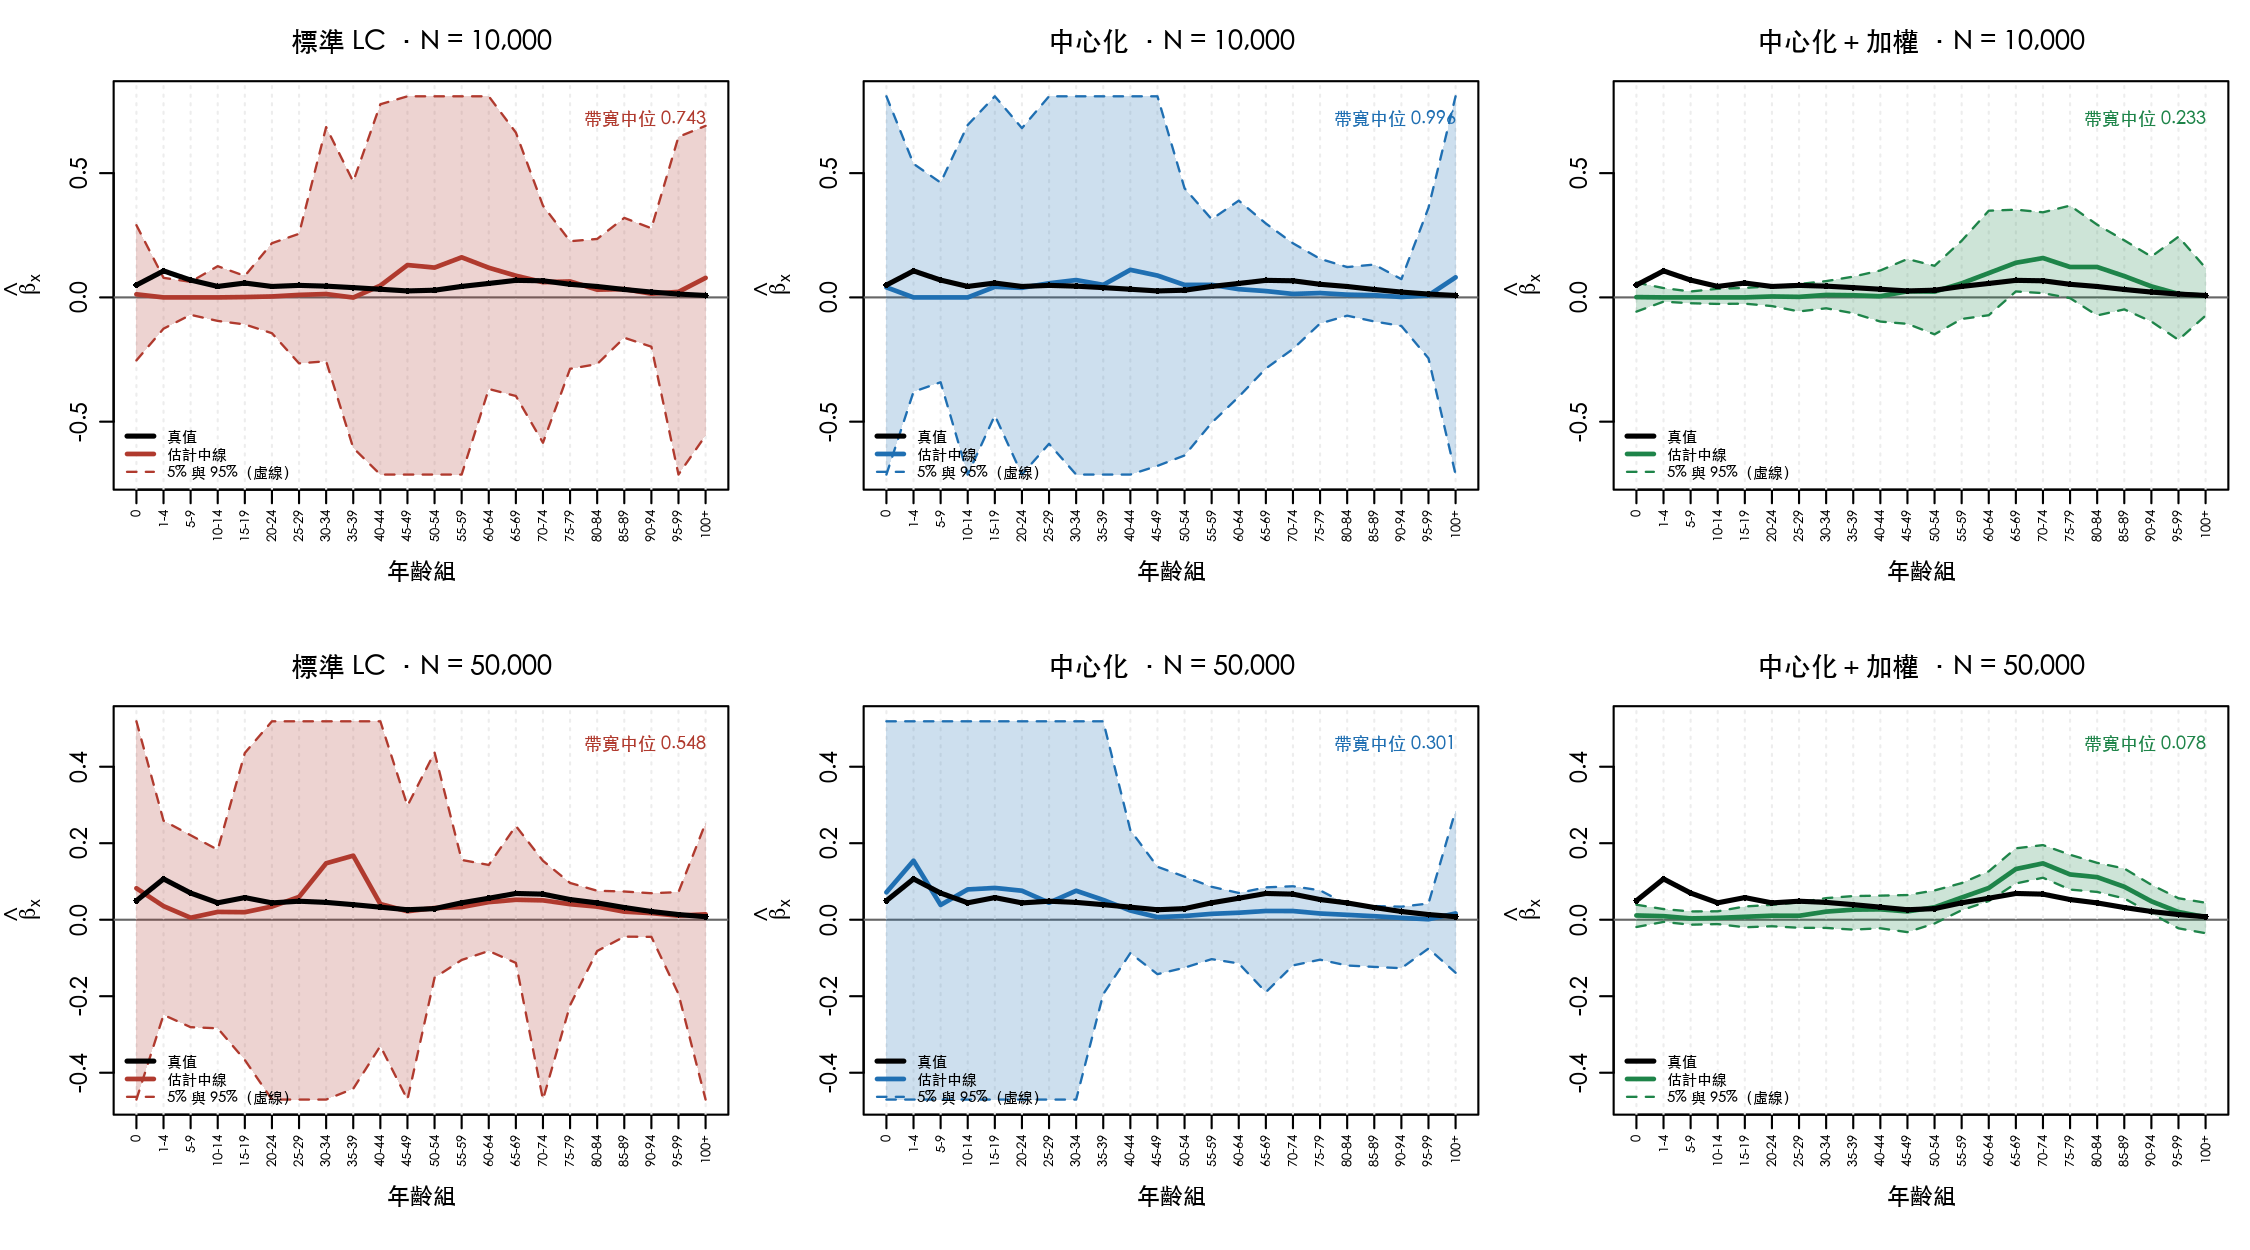
\includegraphics[width=\textwidth]{figT2_beta_band.png}
\caption{$\hat\beta_x$ 的 5--95\% 帶（每格一個估計量，上列 $N=10^4$、
下列 $N=5\times10^4$）。黑線為真值。與圖~\ref{fig:aband} 的 $\alpha$ 相反，
$\beta$ 的帶\textbf{很寬}而中線大致罩住真值，是變異數主導的樣子。
中心化單獨反而使帶\textbf{變寬}（$0.743\to0.996$），
須加上資訊加權才收窄（$\to0.233$）。}
\label{fig:bband}
\end{figure}

兩圖並列即本文的核心對照。$\alpha_x$ 的帶窄而偏離真值，
$\beta_x$ 的帶寬而大致罩住真值：人數五萬時 $\alpha$ 的最大偏誤 $0.866$
是其帶寬 $0.218$ 的\textbf{四倍}，而 $\beta$ 的中線離真值中位僅 $0.011$、
帶寬卻達 $0.548$，相差\textbf{五十倍}。這兩個比值正是
表~\ref{tab:betadec} 確定性佔比（$97\%$ 對 $5.8\%$）的另一種表達，
也說明為何同一個校正對兩者的效果截然不同。

圖~\ref{fig:bband} 另顯示兩項須一併記載的結果。其一，中心化單獨使用時
$\beta$ 的帶反而變寬（人數一萬時 $0.743\to0.996$），視覺上比
表~\ref{tab:estcmp} 的 SSE 數字更直接——校正所注入的 $\hat\mu$ 噪音
在 $\beta$ 上是淨損失。其二，中心化加上加權雖使帶寬大幅收窄
（人數五萬時 $0.548\to0.078$，七倍），但其中線在 60 至 85 歲一段
明顯高於真值（中線離真值的中位由 $0.011$ 升至 $0.036$），
亦即它是以\textbf{偏誤換變異數}，而非同時改善兩者。
相較之下 Firth 在人數五萬時的帶寬為 $0.153$、中線離真值僅 $0.003$，
兩者兼得——這也是第\ref{sec:result}中 Firth 在多數指標上仍勝出的原因。

綜合上述，「能不能在某些假設下降低偏誤」這個問題的答案可寫成兩個條件式，
而兩者互不涵蓋。
其一，若\textbf{Poisson 假設成立}，則 $\alpha_x$ 的偏誤可由式~\eqref{eq:bform}
算出並扣除，改善幅度由表~\ref{tab:betadec} 的確定性佔比給出上界
（人數一萬與五萬時接近全部）。其二，若\textbf{加權後各格的噪音變異數
大致相等}，則 $\beta_x$ 與漂移項的隨機成分可在一階上移除；
但此條件無法由本文的閉式提供，須另行處理。兩個條件互不涵蓋，
這也是小人口 LC 需要兩種藥的原因。

\subsection{與既有修正方法的關係}

最後把本文的校正放回式~\eqref{eq:general} 的分類中，以釐清它與既有補救的
關係。先把該式的損失函數寫清楚。M-分位數的損失為
\begin{equation}\label{eq:mq}
\rho_{\tau,c}(u)=2\,w_\tau(u)\,\psi_c(u),\qquad
w_\tau(u)=\begin{cases}\tau & u>0\\ 1-\tau & u\le 0\end{cases},\qquad
\psi_c(u)=\begin{cases}u^2/2 & |u|\le c\\ c|u|-c^2/2 & |u|>c,\end{cases}
\end{equation}
其中 $\tau$ 控制非對稱、$c$ 控制穩健程度。其兩個極限可直接驗證：
$c\to\infty$ 時 $\psi_c(u)=u^2/2$ 對所有 $u$ 成立，故
$\rho_{\tau,c}(u)=w_\tau(u)u^2$，即 Newey and Powell（1987）的非對稱
最小平方，而 $\tau=0.5$ 時 $w_\tau\equiv0.5$，$\rho$ 退化為 $u^2/2$；
$c\to0$ 時 $\psi_c(u)\to c|u|$，故 $\rho_{\tau,c}(u)\to 2c\,w_\tau(u)|u|$，
而 $w_\tau(u)|u|=u\{\tau-\mathbf{1}(u<0)\}$ 恰為 Koenker and Bassett
（1978）的檢查函數，常數 $2c$ 不影響極小值的位置。
把 $\tau=0.5$、$c=\infty$、$w\equiv1$、$\lambda=0$ 代入式~\eqref{eq:general}
即得式~\eqref{eq:lcobj}，標準 LC 因此是該族的一個角落。

由此角落出發，小人口的各種補救各自改動了其中一項設定：把 $c$ 調成有限或把
$\tau$ 調離 $0.5$ 即得穩健損失；把 $w$ 取為 $\hat\mu$ 即得資訊加權；
把 $\lambda$ 調離零即得 Ridge、LASSO 或經驗貝氏收縮。
問題是這三者與本文的中心化是什麼關係。

關鍵的觀察是三項設定都不改變母體估計方程在真值處的值。就損失形狀而言，
把 $\psi$ 換成 $\psi_{\tau,c}=\rho_{\tau,c}'$ 之後，母體估計方程變為
$\Ex[\psi_{\tau,c}(u(\theta_0))]$，其值一般\textbf{仍不為零}——
事實上因 $\psi_{\tau,c}$ 非線性，該值與 $b$ 的關係還更複雜，
故問題不但沒解決，連「該扣多少」都不再有閉式。就權重而言，
式~\eqref{eq:pop} 在加權後為 $\sum_{x,t}w_{x,t}\Ex[\psi(u_{x,t})]=
\sum_{x,t}w_{x,t}\,b(\mu_{x,t};c_0)$，這是 $b$ 的加權和；
除非權重恰好使該和為零（而那需要事先知道 $b$，即已經做了本文的計算），
否則它同樣不為零。就懲罰而言，$\lambda P(\theta)$ 在解的位置上加一個朝
收縮目標的拉力，這改變的是 $\theta^{\ast}$ 相對於母體估計方程解的位置，
而非母體估計方程本身；它以一個\textbf{新的}偏誤（收縮偏誤）去交換變異數，
並不移除原有的那一項。

三者因此都作用在一個\textbf{已經 Fisher 不一致}的估計方程上，
而式~\eqref{eq:center} 的中心化則直接處理不一致本身。
用式~\eqref{eq:pop} 的語言說，三項設定改變的是估計方程的\textbf{形狀}
（$\psi$）與\textbf{權重}（$w$），中心化改變的是它的\textbf{位置}，
兩者在該式中出現在不同的地方，故彼此正交。

\subsection{加權的最適形式}\label{sec:weight}

式~\eqref{eq:general} 的三項設定中，權重 $w$ 是唯一在本文最終建議中被實際
調動的一個，故其最適形式值得單獨推導。設損失為 $\rho$、$\psi=\rho'$，
逐格權重為 $w_{x,t}$，則加權後的估計方程為
$\sum_{x,t}w_{x,t}\psi(u_{x,t})\,\partial u_{x,t}/\partial\theta=0$。
依 $M$-估計的標準三明治公式，其漸近變異數為 $A^{-1}BA^{-1}$，其中
\[
A=\sum_{x,t} w_{x,t}\,\Ex[\psi'(u_{x,t})]\,g_{x,t}g_{x,t}^{\top},\qquad
B=\sum_{x,t} w_{x,t}^{2}\,\Ex[\psi(u_{x,t})^{2}]\,g_{x,t}g_{x,t}^{\top},
\]
而 $g_{x,t}=\partial u_{x,t}/\partial\theta$。對 $w$ 極小化該變異數，
即得
\begin{equation}\label{eq:wopt}
w\;\propto\;\frac{\Ex[\psi'(u)]}{\Ex[\psi(u)^{2}]} .
\end{equation}
式~\eqref{eq:wopt} 是一個一般結果，把不同的損失代入即得各自的最適權重。
設 $u\sim N(0,\sigma^2)$，三種損失的結果列於表~\ref{tab:wcases}。

\begin{table}[H]
\centering
\caption{三種損失的變異數最適權重
（$\beta_z=\Ex[\min(Z^2,z^2)]$，$Z\sim N(0,1)$；$f$ 為 $u$ 的密度）}
\small
\begin{tabular}{lllll}
\toprule
損失 & $\psi(u)$ & $\Ex[\psi'(u)]$ & $\Ex[\psi(u)^2]$ & 最適權重\\
\midrule
最小平方 & $u$ & $1$ & $\sigma^2$ & $1/\sigma^2$\\
檢查函數 & $\tau-\mathbf{1}(u<0)$ & $f(0)$ & $\tau(1-\tau)$ & $f(0)$\\
Huber$(c)$ & $\min(|u|,c)\,\mathrm{sgn}(u)$ & $2\Phi(c/\sigma)-1$
  & $\sigma^2\beta_{c/\sigma}$ & $\dfrac{2\Phi(c/\sigma)-1}{\sigma^2\beta_{c/\sigma}}$\\
\bottomrule
\end{tabular}
\label{tab:wcases}
\end{table}

第一列即加權最小平方的標準結果。第二列則是 Koenker（2005，第 5.3 節）
定理 5.1 的內容，值得特別指出，因為它與直覺相反：對檢查函數而言，
權重應取該分位處的\textbf{局部密度}而非標準差的倒數，兩者一般並不相同；
本文原先的實作即誤用了後者。第三列的 Huber 損失介於兩者之間，
其形式同時含 $\sigma$ 與截點 $c$，因而是三者中唯一能顯示兩端如何銜接的。
把第三列移到本問題上即得本文所需的形式：由 Poisson 的 delta 方法，
$\mathrm{Var}(\log\hat m_{x,t})\approx1/\mu_{x,t}$，
故 $\sigma_x=\mu_x^{-1/2}$、$c/\sigma_x=c\sqrt{\mu_x}$，代入得
\begin{equation}\label{eq:woptmu}
w_x\;\propto\;\mu_x\,\frac{2\Phi(c\sqrt{\mu_x})-1}{\beta_{c\sqrt{\mu_x}}} .
\end{equation}
式~\eqref{eq:woptmu} 的兩個極限說明了它的結構。$c\sqrt{\mu}\to\infty$ 時
$2\Phi-1\to1$ 且 $\beta\to1$，故 $w\propto\mu$，即最小平方的權重；
$c\sqrt{\mu}\to0$ 時令 $z=c\sqrt{\mu}$，由泰勒展開
$2\Phi(z)-1\approx z\sqrt{2/\pi}$，而 $\beta_z=\Ex[\min(Z^2,z^2)]\approx z^2$
（因 $z$ 小時 $\min(Z^2,z^2)$ 幾乎總是 $z^2$），故
$w\propto\mu\cdot z/z^{2}=\mu/z\propto\sqrt{\mu}$，即檢查函數的權重——
這與第二列一致，因為 $\log\hat m$ 在中位數處的密度為 $\sqrt{\mu/2\pi}$。

由此可得一項結構性的結論：最適權重在 $\sqrt{\mu}$ 與 $\mu$ 之間內插，
而內插的變數是 $c\sqrt{\mu}$ 而非 $c$。因此固定冪次 $w=\mu^{p}$
原則上不可能最適——同一筆資料的各年齡 $\mu$ 橫跨三個數量級，
$c\sqrt{\mu}$ 因而橫跨兩個數量級，式~\eqref{eq:woptmu} 的隱含冪次在
$c=1.345$ 時由 $0.61$ 漂移至 $0.87$，單一冪次只能是某種折衷。
此一預測的實測結果見第\ref{sec:result}末。

\subsection{分布假設的敏感度分析}\label{sec:normal}

上述推導全部建立在式~\eqref{eq:pois} 的 Poisson 假設上，而 $M$-估計的既有
理論多以連續、常態的誤差為設定；既然文獻在常態一側發展得更成熟，
一個自然的問題是能不能改以常態假設推導，以便直接套用那些結果。
答案是一半可以、一半不可以，而分界線恰好落在本問題最關鍵的地方。
可以的那一半是\textbf{加權}。第\ref{sec:weight}的最適權重推導
（式~\eqref{eq:wopt} 與表~\ref{tab:wcases}）全程假設 $u\sim N(0,\sigma^2)$，
其結果與 Poisson 無關，只用到 $\mathrm{Var}(\log\hat m_{x,t})\approx1/\mu_{x,t}$
這個由 delta 方法得來的近似。該部分因而完全落在既有文獻的常態框架內。

不可以的那一半是\textbf{偏誤}。若設
$\ell_{x,t}\sim N\!\big(\log m_{x,t}-\tfrac{1}{2\mu_{x,t}},\,1/\mu_{x,t}\big)$
——這是 $\log(D/E)$ 在 $\mu$ 大時的標準常態近似——則母體估計方程在真值處
的值為
\begin{equation}\label{eq:bnormal}
b_N(\mu)=-\frac{1}{2\mu},
\end{equation}
亦即式~\eqref{eq:jensen} 的一階項。此式簡潔且完全落在常態框架內，
但它\textbf{沒有零格分支}——常態分布取到零的機率為零，
「以 $c_0$ 替代」這件事在常態模型裡根本不存在，因而無從表達。
表~\ref{tab:normal} 把兩者並列。

\begin{table}[H]
\centering
\caption{常態假設下的 $b_N(\mu)=-1/(2\mu)$ 與 Poisson 精確值的比較（$c_0=0.5$）}
\small
\begin{tabular}{rrrrrr}
\toprule
$\mu$ & $P(D=0)$ & Poisson 式~\eqref{eq:bform} & 常態 式~\eqref{eq:bnormal}
 & 差 & 常態的相對誤差\\
\midrule
0.1   & 0.905 & $1.6787$  & $-5.0000$ & $6.679$  & $-398\%$\\
0.3   & 0.741 & $0.7176$  & $-1.6667$ & $2.384$  & $-332\%$\\
0.5   & 0.607 & $0.3416$  & $-1.0000$ & $1.342$  & $-393\%$\\
0.9234& 0.397 & $0.0000$  & $-0.5415$ & $0.542$  & ---\\
2.0   & 0.135 & $-0.1874$ & $-0.2500$ & $0.063$  & $-33\%$\\
5.0   & 0.007 & $-0.1199$ & $-0.1000$ & $-0.020$ & $+17\%$\\
10.0  & 0.000 & $-0.0552$ & $-0.0500$ & $-0.005$ & $+9\%$\\
100.0 & 0.000 & $-0.0050$ & $-0.0050$ & $0.000$  & $+0.8\%$\\
\bottomrule
\end{tabular}
\label{tab:normal}
\end{table}

表~\ref{tab:normal} 的意思很清楚：常態假設給出的偏誤公式在 $\mu>9.5$ 時
相對誤差小於一成，對死亡數以十計以上的年齡完全夠用；
但在 $\mu<1$ 的年齡，它不僅量級錯誤，\textbf{連正負號都相反}——
$\mu=0.3$（即人數五萬時的幼年組）時常態給 $-1.667$ 而實際為 $+0.718$。
原因是常態框架看不見零格替代這個機制，只保留了 Jensen 不等式那一項，
而在小 $\mu$ 處主導的恰是前者。

因此本文的取捨是：加權的部分用常態，偏誤的部分必須用 Poisson 。
這個分工並非權宜，而是反映兩者所刻畫的東西不同——加權處理的是變異數的
異質，那是二階動差的性質，常態近似已足；偏誤處理的是轉換與替代對一階
動差的影響，而替代規則的效果只在離散分布上才存在。
這一點也說明為何既有文獻在常態框架下發展得更成熟卻未觸及本文的問題：
在其標準應用場景中，反應變數本就是連續的，不會出現「必須把零替換掉」
這個步驟。

此一分類給出兩項可檢驗的預測，第\ref{sec:result}將逐一檢驗。
其一，中心化應可大幅移除 $\alpha_x$ 的偏誤，因為 Fisher 不一致正發生在
式~\eqref{eq:svd} 定義 $\hat\alpha_x$ 的那個平均上。
其二，中心化\textbf{不應}改善時間參數的漂移項——漂移項的誤差來自
等權重的秩一分解對異質變異的敏感，屬於權重 $w$ 這項設定的範疇，
而非估計方程中心的範疇。

\subsection{模擬設定與計算環境}\label{sec:setup}

第\ref{sec:valid}與第\ref{sec:result}的所有模擬共用同一組設定，為免重複，
此處一次寫定。

\textbf{資料與真值。} 資料取自 Human Mortality Database 的臺灣女性
2001 至 2024 年死亡數與曝露數，聚合為 $A=22$ 個五齡組（$0$、$1$--$4$、
$5$--$9$、\dots、$95$--$99$、$100^{+}$），年份數 $T=24$。
真值定義為全國資料的 Poisson 最大概似配適
$(\alpha^{0}_x,\beta^{0}_x,\kappa^{0}_t)$，其隱含的死亡率為
$m^{0}_{x,t}=\exp(\alpha^{0}_x+\beta^{0}_x\kappa^{0}_t)$。
以配適值而非觀測值為真值的理由是：本文所要檢驗的是估計程序對給定
$\mu_{x,t}$ 的反應，故真值必須落在模型內；觀測值偏離模型的影響另於
第\ref{sec:real}單獨處理。

\textbf{性別。} 全部模擬只用女性。理由有二：女性的死亡率曲線較平滑、
偏離秩一結構的程度較小，可使驗證聚焦於推導本身；
而本文的閉式只透過期望死亡數進入偏誤，性別本身不是閉式中的變數，
男性的差異僅反映為 $\mu_{x,t}$ 水準的不同，
故以女性為例不失一般性。全性別合併的情形因兩性死亡率型態不同而需另設模型，
本文不予處理。

\textbf{人口規模與年齡結構。} 曝露數設為 $E_{x,t}=N\,w_x$，
其中 $N$ 為單一性別的總人數、$w_x$ 為年齡結構。
除第\ref{sec:valid}之三另行指定者外，$w_x$ 一律取 2024 年全國女性的
曝露結構（$65$ 歲以上占 $20.3\%$），且不隨年份變動，
以使不同規模之間的比較只反映人數的差異。
人數取 $N\in\{10^4,\,5\times10^4,\,2\times10^5\}$，
涵蓋臺灣鄉鎮市區的主要範圍：368 個鄉鎮市區中有 217 個的單一性別人數在
兩萬以下、299 個少於五萬。

\textbf{重複與亂數。} 各組合重複 $R=100$ 次，死亡數依式~\eqref{eq:pois}
以 \texttt{rpois} 產生。亂數種子固定為
$\text{seed}=20260926+1000\,i+r$，其中 $i$ 為人口規模的序號、
$r$ 為重複的序號；第\ref{sec:valid}、第\ref{sec:result}之二至之四
與第\ref{sec:joint}沿用同一組種子，故各表可逐格對照，
不同估計量之間的差異不含蒙地卡羅的雜訊。
第\ref{sec:result}之五（參考母體）與之六（真實資料抽薄）因需額外的亂數，
採 $20260926+11000\,i+97\,s+r$ 與 $20260926+7000\,i+r$ 兩組，
其中 $s$ 為情境的序號。

\textbf{比較指標。} 四項指標分別對應四個標的。
$\alpha$ 的偏誤取各年齡 $\hat\alpha_x-\alpha^{0}_x$ 在 $R$ 次重複中的中位數，
再取其絕對值的中位數與最大值，前者刻畫整體水準、後者刻畫最差的年齡。
$\beta$ 的誤差取相對平方誤差和
$\mathrm{SSE}(\beta)=\sum_x(\hat\beta_x-\beta^{0}_x)^2\big/\sum_x(\beta^{0}_x)^2$。
時間參數以漂移項 $(\hat\kappa_T-\hat\kappa_1)/(T-1)$ 與真值之差表示。
最終標的為配適末年的零歲平均餘命，依均勻死亡假設編算簡易生命表，
最高年齡組為 $100$ 歲以上，其平均餘命取 $1/m_{A}$。
離散度另以 $R$ 次重複的標準差、四分位距與全距表示。

\textbf{計算環境。} 全部計算在 R 4.2.1（x86\_64-apple-darwin17.0）下完成。
除讀取 Excel 檔的 \texttt{readxl} 與稀疏矩陣的 \texttt{Matrix} 外，
不依賴任何外部套件；本文所比較的各估計量——標準 LC、 Poisson 最大概似、
Firth 預先修正、中心化校正、資訊加權、partial SMR 與 Whittaker 比值修勻
——皆為自行實作，程式置於 \texttt{R/core/} 與 \texttt{R/studies/}，
各節所引的表格編號與產生該表的程式檔名一一對應。
奇異值分解採 R 內建的 \texttt{svd}（LAPACK）， Poisson 配適採自行撰寫的
疊代重加權最小平方，收斂門檻為參數變動的最大絕對值小於 $10^{-10}$。

\section{以臺灣資料驗證閉式}\label{sec:valid}

\subsection{驗證的設計}

Corollary~\ref{cor:alpha} 是一個恆等式，因此嚴格說來並不需要驗證：
只要式~\eqref{eq:pois} 的 Poisson 假設成立、且 $\hat\alpha_x$ 依
式~\eqref{eq:svd} 定義為列平均，該式就必然成立。但這兩個前提在實際的估計
流程中未必如字面那樣單純。一方面，實際的 LC 配適含奇異值分解與識別條件的
正規化，而 $\sum_x\hat\beta_x=1$ 與 $\sum_t\hat\kappa_t=0$ 這兩個約束是在
分解之後才施加的，其重新尺度化是否會把 $\hat\alpha_x$ 也帶動，
單看推導並不明顯；另一方面，推導把 $\beta_x\kappa_t$ 當成已知的真值，
而實際上它們也是估計出來的，兩者的誤差是否會滲入 $\hat\alpha_x$，
同樣須以數值確認。本節因此不是在檢驗數學，而是在檢驗\textbf{推導所描述的
那個量，是否確實就是實際估計流程所產生的那個量}。

資料、真值、人口規模與亂數種子均依第\ref{sec:setup}所定。
此一設計有兩項代價須先承認。其一，它假設小人口的
死亡率\textbf{恰好}等於全國的死亡率，而真實的鄉鎮市區顯然不是如此；
但本節的目的是檢驗閉式，而閉式所刻畫的是估計程序對給定 $\mu_{x,t}$ 的
反應，與該 $\mu_{x,t}$ 是否貼近某個真實地區無關。其二，它使資料恰好落在
秩一雙線性結構上，因而排除了模型誤設；這一點在本節是優點——
若連如此單純的情形都無法吻合，推導即有問題——但也使本節的結論須由
第\ref{sec:real}補上另一半。

每一次重複皆以標準 LC 估計，取各年齡 $\hat\alpha_x-\alpha^{0}_x$ 在 100 次
重複中的中位數作為該年齡的實測偏誤，再與 Corollary~\ref{cor:alpha} 的
預測值 $\bar b_x=T^{-1}\sum_t b(\mu_{x,t};c_0)$ 比較。
比較的方式有二：逐年齡的相關係數，以及以預測值為自變數、實測值為應變數的
迴歸斜率；前者檢驗\textbf{形狀}是否一致，後者檢驗\textbf{量級}是否一致。
兩者都接近 $1$ 才算通過。

\subsection{閉式預測與模擬實測的對照}

\begin{table}[H]
\centering
\caption{閉式預測與模擬實測的對照（標準 LC，重複 100 次）}
\small
\begin{tabular}{lrrr}
\toprule
 & $N=10^4$ & $N=5\times10^4$ & $N=2\times10^5$\\
\midrule
逐年齡的相關係數 & \textbf{1.000} & \textbf{1.000} & \textbf{0.988}\\
迴歸斜率（實測對預測） & 1.001 & 0.990 & 0.962\\
殘差量級 & $\sim$0.01 & $\sim$0.01 & $\sim$0.02\\
\bottomrule
\end{tabular}
\label{tab:valid}
\end{table}

表~\ref{tab:valid} 顯示形狀與量級都通過。逐年齡的相關係數在三個規模下
分別為 $1.000$、$1.000$、$0.988$，迴歸斜率為 $1.001$、$0.990$、$0.962$，
兩者都接近 $1$；殘差的量級約為 $0.01$ 至 $0.02$，而重複 100 次時
$\alpha$ 偏誤的蒙地卡羅誤差本就約有一成，以人數五萬時 5 至 9 歲組的
$0.87$ 計即約 $0.09$，故 $0.01$ 的殘差已在雜訊之內。
人數二十萬時相關係數與斜率略低（$0.988$ 與 $0.962$），
原因是該規模下各年齡的絕對偏誤已降到 $0.1$ 以下，
蒙地卡羅誤差相對於待測的量變大，並非推導本身在該處失準。

表~\ref{tab:validage} 進一步列出逐年齡的對照，而這張表同時展示了
第\ref{sec:normal}前所導出的兩個門檻。先看中位數的崩潰門檻
$\mu<\ln2=0.693$：1 至 4 歲、5 至 9 歲、10 至 14 歲三組的單年期望死亡數
皆為 $0.3$，其零格比例 $\pi=e^{-0.3}=0.74$ 已遠超過 $50\%$，
15 至 19 歲組的 $0.5$ 人對應 $\pi=0.61$ 亦然；
這四組因此落在穩健損失的作用範圍之外，而它們恰好也是偏誤最大的四組
（$0.33$ 至 $0.87$）。再看偏誤的變號門檻 $\mu^\ast=0.9234$：
20 至 24 歲組的期望死亡數為 $0.9$，恰在門檻上，其偏誤因而僅 $+0.04$，
幾乎為零；而零歲組的 $1.2$ 人已越過門檻，偏誤轉為 $-0.07$。
兩個門檻所預測的位置與實測一一對應，且都可由死亡數直接算出，
不需要真值——這正是把閉式寫出來的實用價值所在。

\begin{table}[H]
\centering
\caption{逐年齡對照（$N=5\times10^4$，選列）}
\small
\begin{tabular}{lrrrrr}
\toprule
年齡組 & 單年期望死亡數 & $\pi=e^{-\mu}$ & 閉式預測 & 模擬實測 & 差\\
\midrule
0      & 1.2  & 0.30 & $-0.0753$ & $-0.0692$ & $+0.0061$\\
1--4   & 0.3  & \textbf{0.74} & $0.7283$  & $0.7135$  & $-0.0148$\\
5--9   & 0.3  & \textbf{0.77} & $0.8689$  & $0.8658$  & $-0.0031$\\
10--14 & 0.3  & \textbf{0.77} & $0.8341$  & $0.8262$  & $-0.0079$\\
15--19 & 0.5  & \textbf{0.61} & $0.3298$  & $0.3386$  & $+0.0088$\\
20--24 & 0.9  & 0.41 & $0.0415$  & $0.0529$  & $+0.0114$\\
45--49 & 7.3  & 0.00 & $-0.0793$ & $-0.0831$ & $-0.0038$\\
70--74 & 48.8 & 0.00 & $-0.0108$ & $-0.0135$ & $-0.0027$\\
85--89 & 73.9 & 0.00 & $-0.0069$ & $-0.0061$ & $+0.0008$\\
\bottomrule
\end{tabular}
\label{tab:validage}
\end{table}

圖~\ref{fig:aband} 把同一件事畫出來，而圖比表更能說明偏誤與變異的相對
大小。圖中紅色區域為標準 LC 在 100 次重複中 $\hat\alpha_x-\alpha_x$ 的
$5$ 至 $95$ 百分位帶，紅線為其中線，黑色虛線則是Corollary~\ref{cor:alpha}
的閉式預測 $\bar b_x$。

\begin{figure}[H]
\centering
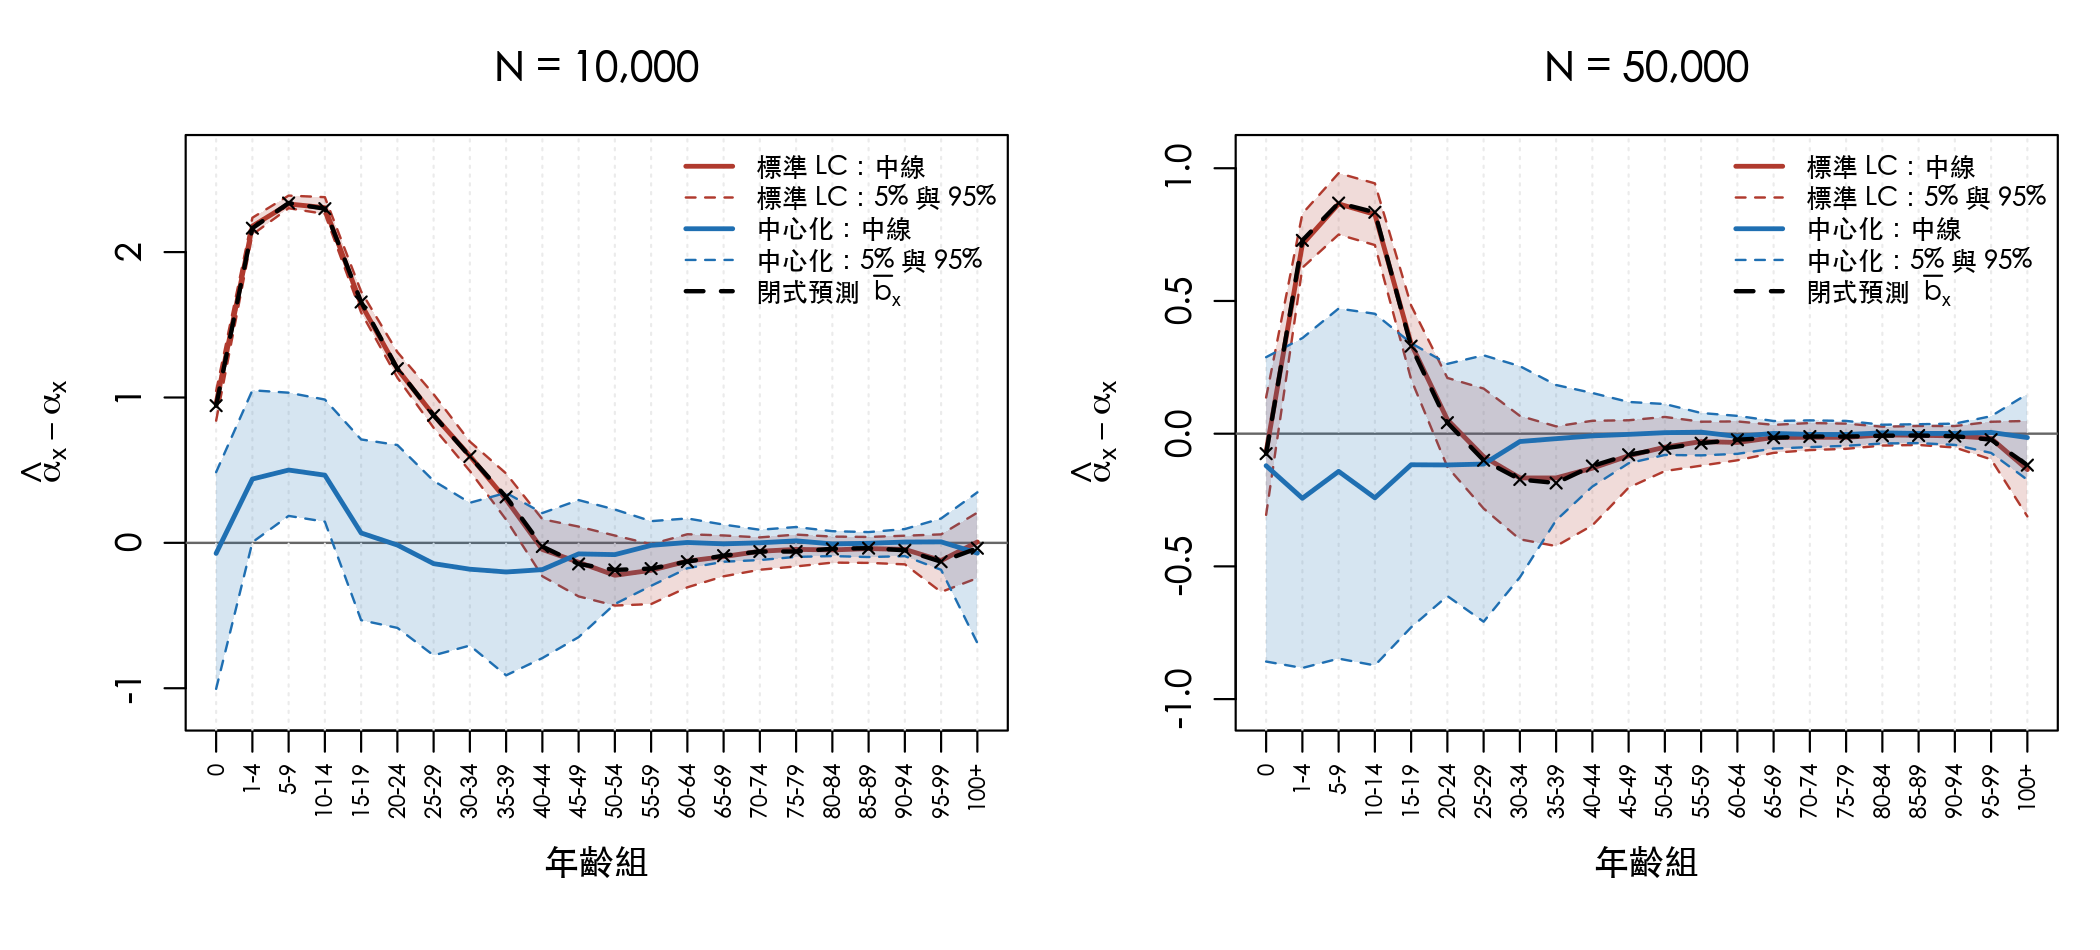
\includegraphics[width=\textwidth]{figT1_alpha_band.png}
\caption{$\hat\alpha_x$ 的偏誤：5--95\% 帶與閉式預測。黑色虛線為
Corollary~\ref{cor:alpha} 的預測值 $\bar b_x$，與標準 LC 的中線幾乎完全重合
（最大差 $0.043$ 與 $0.019$）。標準 LC 的帶\textbf{窄}而整條\textbf{偏離
零}，是偏誤主導的樣子；中心化（藍）把中線拉回零附近，代價是帶變寬。}
\label{fig:aband}
\end{figure}

圖~\ref{fig:aband} 有三點可讀。第一，\textbf{黑色虛線落在紅線上}：
閉式預測與模擬中線的最大差在兩個規模下分別為 $0.043$ 與 $0.019$，
而偏誤本身在 5 至 9 歲組達 $2.33$ 與 $0.87$。這是Corollary~\ref{cor:alpha}
的視覺版本。第二，\textbf{標準 LC 的帶很窄}——人數五萬時帶寬中位為
$0.218$，而 5 至 9 歲組的偏誤為 $0.866$，偏誤是帶寬的四倍。
亦即該年齡幾乎每一次模擬都落在真值的同一側，這正是「偏誤主導」的
操作型定義，也說明為何重複抽樣無法察覺它。第三，中心化（藍）把中線
拉回零附近，但帶變寬（人數五萬時 $0.218\to0.277$）——這是以 $\hat\mu$
代入所注入的噪音，屬第\ref{sec:result}所述的代價。

綜合表~\ref{tab:valid}、表~\ref{tab:validage} 與圖~\ref{fig:aband}，
本節的結論是推導所描述的量確實就是實際估計流程所產生的量：
奇異值分解與識別條件的正規化並未把 $\hat\alpha_x$ 帶動，
$\hat\beta$ 與 $\hat\kappa$ 的估計誤差也未明顯滲入。
這把先前只能以模擬描述的現象變成一個可計算的量——標準 LC 的 $\alpha_x$
偏誤\textbf{完全}由各格期望死亡數的一個確定性函數決定，不含未知成分。
既然如此，該量即可計算並扣除，此即下一節的工作。
須補充的是，本節情境的單純性係由設計而來：資料恰好落在秩一結構上、
分布恰好是 Poisson 。真實資料兩者都不完全成立，
故第\ref{sec:real}將以實際觀測的死亡數重做一次，檢驗結論是否仍然成立。

\subsection{人口年齡結構的影響}\label{sec:popstr}

前一小節的驗證在單一的年齡結構下進行。但閉式 $b(\mu;c_0)$ 只透過期望死亡數
$\mu_{x,t}=E_{x,t}m_{x,t}=N w_x m_{x,t}$ 進入偏誤，而 $w_x$ 正是年齡結構；
因此閉式對本問題給出一個更嚴格的可檢驗預測：
\textbf{在總人數 $N$ 固定下改變 $w_x$，標準 LC 的逐年齡偏誤應隨之改變，
且改變的方向與幅度完全由 $b(\mu)$ 決定}。
這比「偏誤是否隨 $N$ 變化」更嚴格，因為此處資訊總量不變，
變的只是資訊在年齡之間的分配。本小節檢驗此一預測，
並一併回答鄉鎮市區應用上的實務問題：同樣是五萬人的地區，
人口老化的程度是否會改變 LC 估計的可信度。

三組結構皆以臺灣女性的實際曝露數為本。年輕結構取 2001 年的全國結構
（$65$ 歲以上占 $8.5\%$），基準結構取 2024 年（$20.3\%$），
高齡結構則以 2024 年結構作指數傾斜 $w_x\propto w_x^{2024}e^{0.085(x-1)}$，
使 $65$ 歲以上占 $31.7\%$，對應人口外流的鄉鎮市區。
三者的總人數相同，真實死亡率 $m^{0}_{x,t}$ 亦相同，差別只在年齡分配。

\begin{table}[H]
\centering
\caption{人口年齡結構對偏誤的影響（$N=5\times10^4$，重複 100 次）}
\small
\renewcommand{\arraystretch}{1.15}
\begin{tabular}{llrrrrr}
\toprule
結構 & 估計量 & $\alpha$ 中位 & $\alpha$ 最大 & SSE($\beta$) & $e_0$ 偏誤 & $e_0$ 標準差\\
\midrule
\multirow{3}{*}{年輕（$65^{+}$ 占 $8.5\%$）}
 & 標準 LC      & 0.0907 & 0.4275 & 4.2032 & $-1.055$ & 0.897\\
 & Firth        & 0.0111 & \textbf{0.0416} & 1.3418 & $-0.318$ & 0.838\\
 & 中心化＋加權 & 0.0393 & 0.0865 & \textbf{1.0960} & \textbf{$-0.235$} & 0.973\\
\addlinespace
\multirow{3}{*}{基準（$20.3\%$）}
 & 標準 LC      & 0.0596 & 0.8658 & 3.9369 & $-1.415$ & 0.626\\
 & Firth        & 0.0057 & \textbf{0.0724} & 1.6656 & $-0.182$ & 0.429\\
 & 中心化＋加權 & 0.0213 & 0.0735 & \textbf{1.1366} & \textbf{$+0.057$} & 0.564\\
\addlinespace
\multirow{3}{*}{高齡（$31.7\%$）}
 & 標準 LC      & 0.0492 & 1.4555 & 6.2652 & $-2.109$ & 0.685\\
 & Firth        & 0.0070 & \textbf{0.1276} & 2.9394 & $-0.210$ & 0.418\\
 & 中心化＋加權 & 0.0187 & 0.1110 & \textbf{1.2424} & \textbf{$+0.066$} & 0.517\\
\bottomrule
\end{tabular}
\label{tab:popstr}
\end{table}

表~\ref{tab:popstr} 給出三項結果。
第一，年齡結構確實影響偏誤，且影響的幅度與人數的影響相當。
同樣是五萬人，標準 LC 的 $\alpha$ 最大偏誤由年輕結構的 $0.428$ 上升到
高齡結構的 $1.456$，約為三點四倍；零歲平均餘命的偏誤由 $-1.055$ 歲
擴大到 $-2.109$ 歲，正好一倍。作為對照，在基準結構下把人數由五萬降到
一萬才使 $e_0$ 偏誤由 $-1.415$ 擴大到 $-3.725$ 歲。
換言之，人口老化對估計品質的傷害，與人口減少是同一個量級的問題。
其機制由閉式直接讀出：高齡結構把曝露數由幼年組移往高齡組，
使幼年組的 $\mu_{x,t}$ 更小、$b(\mu)=\log(c_0/\mu)$ 更大，
而高齡組的 $\mu$ 雖然增加，$b$ 在該端卻只以 $-1/(2\mu)$ 的速率趨近零，
兩端並不對稱，故整體偏誤惡化。

第二，\textbf{閉式在三種結構下都準確}。以 $\bar b_x$ 預測逐年齡實測偏誤，
三種結構的相關係數分別為 $0.998$、$0.999$、$1.000$，
迴歸斜率為 $0.959$、$0.987$、$0.986$；人數一萬時相關係數皆為 $1.000$、
斜率為 $0.995$、$0.996$、$1.001$。
由於三組結構下的 $\mu_{x,t}$ 完全不同，而同一個函數在三組之上都準確，
這比第\ref{sec:valid}之二的單一結構驗證更強：
閉式所捕捉的不是某一組曝露數的巧合，而是估計程序對 $\mu$ 的反應。
這同時給出一個實務上的推論：分析者只要有曝露數與一組初步的死亡率估計，
就可以在不做任何模擬的情形下，事先算出該地區的 LC 估計會偏多少。

第三，\textbf{校正後的結果對結構不敏感}。中心化加權的 $e_0$ 偏誤在三種結構
下分別為 $-0.235$、$+0.057$、$+0.066$ 歲，全距 $0.30$ 歲；
而未校正者為 $-1.055$、$-1.415$、$-2.109$ 歲，全距 $1.05$ 歲。
$\alpha$ 最大偏誤的全距亦由 $1.03$ 降至 $0.025$。
亦即校正不只縮小偏誤，也移除了偏誤對年齡結構的依賴——
這是扣除 $b(\mu_{x,t})$ 的必然結果，因為結構正是透過 $\mu$ 進入偏誤的。
須注意 Firth 在 $\alpha$ 最大偏誤上仍略勝（$0.042$、$0.072$、$0.128$ 對
$0.087$、$0.074$、$0.111$），但在 $\beta$ 與平均餘命上則一致地落後，
此一分工與第\ref{sec:result}之二的結果一致。

人數一萬時的結論則須保留。該規模下中心化加權的 $e_0$ 偏誤為
$-2.542$、$-1.200$、$-0.636$ 歲，雖較標準 LC 的 $-1.858$、$-3.725$、$-6.987$
有大幅改善，但年輕結構下反而劣於標準 LC。
原因是年輕結構把曝露數集中在死亡率極低的年齡，
使該處的 $\hat\mu$ 本身幾無資訊，代入 $b(\hat\mu)$ 後所扣的量遠小於應扣的量；
校正因而在最需要它的地方自動失效。這一點在第\ref{sec:disc}列為限制。

\section{以中心化修改 LC 的估計}\label{sec:result}

\subsection{修改後的估計流程}

式~\eqref{eq:center} 的中心化在實作上是扣除\textbf{格}而非校正參數，
使校正同時流入三個參數。困難在於 $b$ 依賴未知的 $\mu_{x,t}$，故須迭代：

實作上先以標準 LC 起始，得到一組
$(\hat{\boldsymbol\alpha},\hat{\boldsymbol\beta},\hat{\boldsymbol\kappa})$，
據以算出各格的期望死亡數
$\hat\mu_{x,t}=E_{x,t}\exp(\hat\alpha_x+\hat\beta_x\hat\kappa_t)$；
再以 $\ell_{x,t}-b(\hat\mu_{x,t};c_0)$ 取代原始的 $\ell_{x,t}$，
依式~\eqref{eq:svd} 重新配適，得到新的一組參數後回頭更新 $\hat\mu_{x,t}$，
如此反覆至參數的變動小於容忍值為止，實測收斂約需三至六次。
此一迭代之所以必要，是因為式~\eqref{eq:bform} 依賴未知的 $\mu_{x,t}$，
而後者只能由配適值估計；也正因為如此，$\hat\mu$ 的誤差會隨校正一併注入
每一格，構成第\ref{sec:result}末所述的第一項限制。

與偏誤減少文獻的關係值得一提。Firth（1993）把偏誤減少方法分為
\textbf{事後修正}（先算最大概似估計值再扣除偏誤的估計，
即 Cox and Snell 1968）與\textbf{預先修正}（修改估計方程本身，
即 Firth 的 Jeffreys 懲罰）。本文屬前者，但施加對象不同，
而這個不同是決定性的：Cox--Snell 修正的是最大概似估計量的 $O(n^{-1})$
偏誤，前提是最大概似估計值\textbf{存在且有限}；而小人口 LC 的核心困難
正是零格導致的完全分離（Albert and Anderson 1984），
Poisson 最大概似的 $\hat\alpha_x$ 可為 $-\infty$（本文實測人數一萬時
5 至 9 歲組為 $-13.03$），故 Cox--Snell 在此無從施加。
式~\eqref{eq:bform} 則完全不涉及最大概似估計量，只用到 $D$ 的邊際分布。

\subsection{實證結果}

以下的比較採與第\ref{sec:valid}完全相同的亂數種子，故各表可逐格對照。
所比較的五個估計量涵蓋第\ref{sec:limtable}所列的前三項限制：標準 LC 為未修正的
基準， Poisson 最大概似用以呈現事後修正一列所載「須最大概似估計值存在」
這項限制在本問題上的後果，Firth 代表預先修正一路，
中心化與中心化加權則為本文所提的修正。

\begin{table}[H]
\centering
\caption{中心化與既有作法的比較（重複 100 次，取中位數）}
\small
\begin{tabular}{llrrrrr}
\toprule
$N$ & 估計量 & $\alpha$ 中位 & $\alpha$ 最大 & SSE($\beta$) & cor($\beta$) & 漂移偏誤\\
\midrule
\multirow{5}{*}{$10^4$}
 & 標準 LC          & 0.1612 & 2.3309 & 7.916 & $-0.074$ & 0.3436\\
 & Poisson MLE       & 0.0495 & 13.0317 & 15.525 & 0.118 & 0.1612\\
 & Firth            & \textbf{0.0248} & \textbf{0.4267} & 17.797 & 0.116 & 0.2237\\
 & 中心化           & 0.0693 & 0.5008 & 18.048 & $-0.078$ & 0.3544\\
 & 中心化 $+$ 加權   & 0.1749 & 0.7399 & \textbf{2.537} & 0.111 & \textbf{0.1884}\\
\midrule
\multirow{5}{*}{$5\times10^4$}
 & 標準 LC          & 0.0611 & 0.8658 & 4.449 & 0.037 & 0.3339\\
 & Poisson MLE       & 0.0073 & 0.2260 & 1.756 & 0.365 & 0.0492\\
 & Firth            & 0.0088 & \textbf{0.0680} & 1.410 & \textbf{0.397} & \textbf{0.0485}\\
 & 中心化           & \textbf{0.0093} & 0.2434 & 8.834 & 0.198 & 0.3335\\
 & 中心化 $+$ 加權   & 0.0110 & 0.2524 & \textbf{1.023} & 0.179 & 0.1381\\
\midrule
\multirow{5}{*}{$2\times10^5$}
 & 標準 LC          & 0.0231 & 0.1846 & 1.400 & 0.379 & 0.2117\\
 & Poisson MLE       & \textbf{0.0018} & 0.0361 & 0.346 & 0.596 & 0.0267\\
 & Firth            & 0.0025 & \textbf{0.0398} & \textbf{0.333} & \textbf{0.605} & \textbf{0.0262}\\
 & 中心化           & 0.0032 & 0.1778 & 3.499 & 0.438 & 0.2747\\
 & 中心化 $+$ 加權   & 0.0071 & 0.2897 & 0.832 & 0.213 & 0.1106\\
\bottomrule
\end{tabular}
\label{tab:estcmp}
\end{table}

圖~\ref{fig:cmp} 與圖~\ref{fig:e0} 把表~\ref{tab:estcmp} 與
表~\ref{tab:real} 的內容畫出來，前者比較三項參數指標、後者直接看使用者
真正關心的平均餘命。

\begin{figure}[H]
\centering
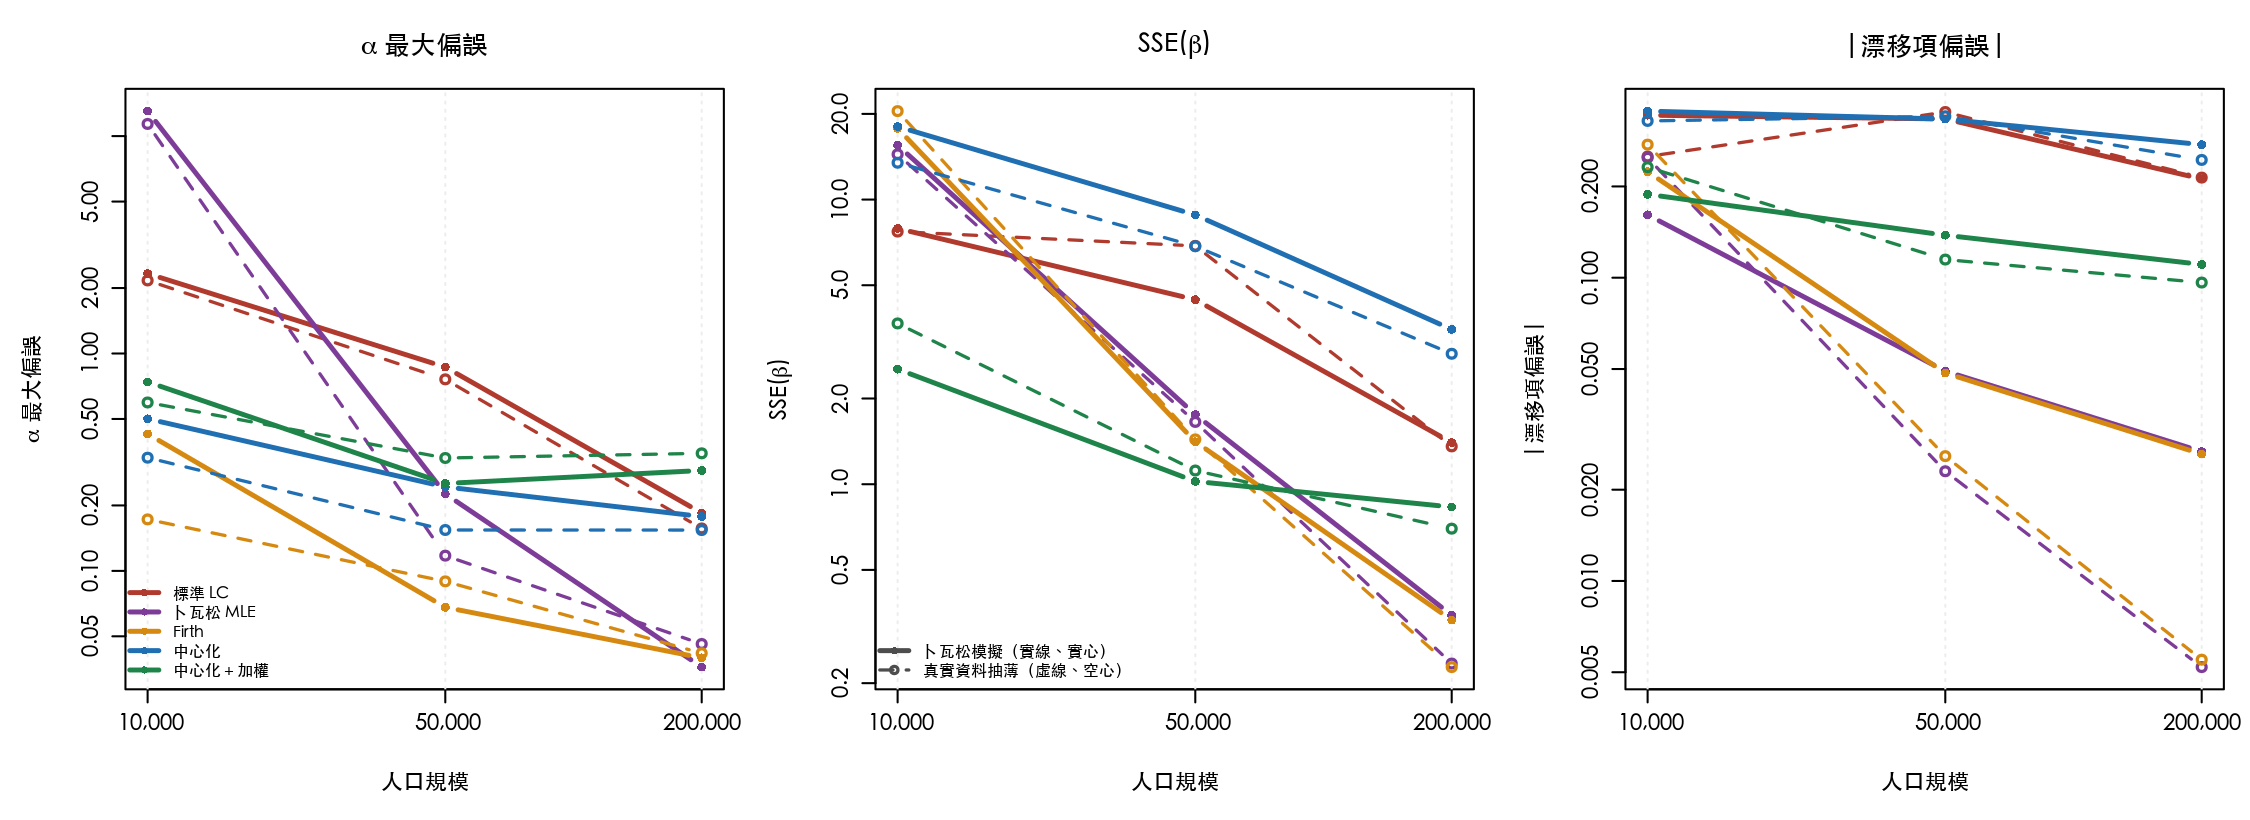
\includegraphics[width=\textwidth]{figT3_estimator_compare.png}
\caption{三項指標隨人口規模的變化（縱軸取對數）。實線與實心點為 Poisson
模擬，虛線與空心點為實際觀測死亡數的 Poisson 抽薄。兩組幾乎平行，
顯示結論不因本資料所含的模型誤設而改變。}
\label{fig:cmp}
\end{figure}

\begin{figure}[H]
\centering
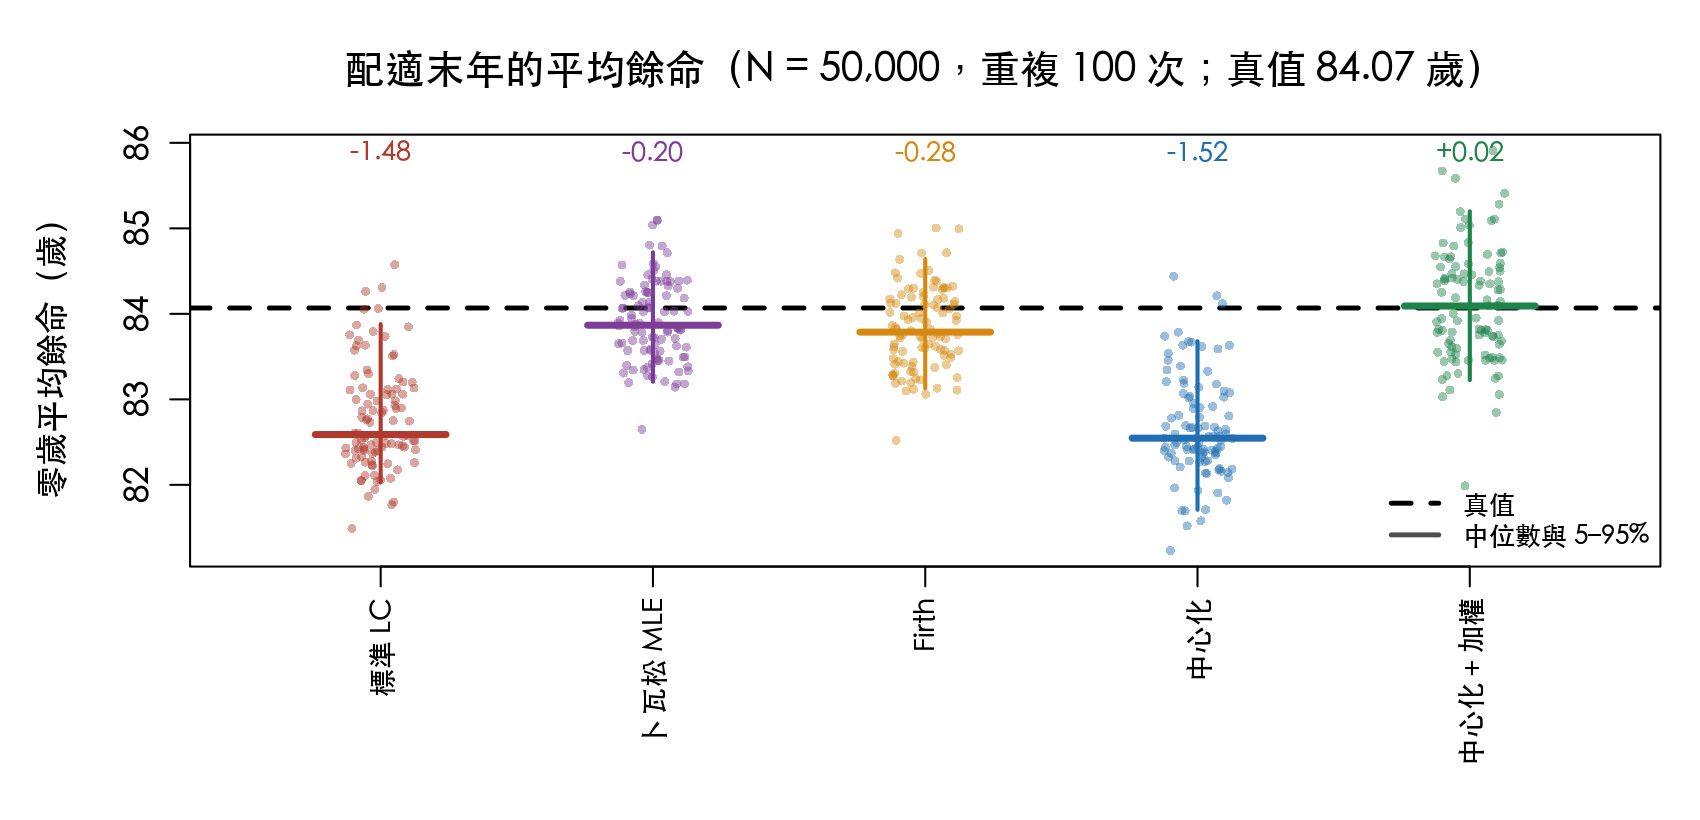
\includegraphics[width=0.78\textwidth]{figT4_e0_by_estimator.png}
\caption{配適末年零歲平均餘命的 100 次重複（$N=5\times10^4$）。
虛線為真值 $84.07$ 歲，各估計量上方標示其中位偏誤。標準 LC 低估 $1.48$ 歲，
中心化加權則為 $+0.02$ 歲。}
\label{fig:e0}
\end{figure}

圖~\ref{fig:cmp} 顯示一項須並列才能辨識的訊息：實線與虛線幾乎平行，
亦即以真實觀測死亡數抽薄所得的結論與純 Poisson 模擬一致；
唯一的例外是標準 LC 的 SSE($\beta$)，其虛線明顯高於實線，
這正是第\ref{sec:real}所述「真實資料中不合秩一結構的成分也被 $\hat\beta$
吸收」的表現。圖~\ref{fig:e0} 則把參數層次的改善翻譯成使用者真正關心的量：
標準 LC 的一百次重複全部落在真值之下，中位數低估 $1.48$ 歲；
Poisson 最大概似與 Firth 分別改善至 $-0.20$ 與 $-0.28$ 歲；
而中心化加權的中位數為 $+0.02$ 歲，點雲已大致對稱地分布在真值兩側。

第\ref{sec:method}末所提的兩項預測都成立，而其中第二項的成立方式比第一項
更有說服力。第一項預測是中心化應大幅移除 $\alpha_x$ 的偏誤：
$\alpha$ 偏誤中位數在三個規模下分別下降 $2.3$、
$6.6$、$7.2$ 倍；人數一萬時 $\alpha$ 最大偏誤由 $2.3309$ 降至 $0.5008$，
且決定性地優於 Poisson 最大概似的 $13.03$——後者因完全分離而崩壞，
這正是式~\eqref{eq:bform} 不依賴最大概似這個性質的價值。
加上資訊加權之後，該估計量在三個規模的每一項指標上都優於標準 LC
（$\beta$ 的平方誤差和 $7.92\to2.54$、$4.45\to1.02$、$1.40\to0.83$；
漂移項偏誤 $0.34\to0.19$、$0.33\to0.14$、$0.21\to0.11$），
且完全留在奇異值分解的架構內、沒有調校參數。

第二項預測是中心化\textbf{不應}改善漂移項，而這一項的成立是本文分工論
最強的證據。漂移項偏誤由 $0.3436$、$0.3339$、$0.2117$ 變為 $0.3544$、
$0.3335$、$0.2747$，即無改善。這與第\ref{sec:method}末的預測一致：
中心化動的是估計方程的中心，而漂移項的誤差來自權重。
既然一個確定性的 $\mu$ 函數可以移除 $\alpha$ 的偏誤卻完全不動漂移項，
那麼漂移項的偏誤就不可能是對數轉換造成的——它須以 $w$ 這個設定處理，
這也正是「中心化 $+$ 加權」一列改善漂移項的原因。

\subsection{逐年齡的改善剖面}\label{sec:ageprof}

前一小節的指標是跨年齡彙總的。但閉式 $b(\mu;c_0)$ 是期望死亡數的函數，
而期望死亡數在年齡之間相差三個數量級，
故閉式對改善的\textbf{分布}也給出預測：
校正的效果應集中在死亡數少的年齡，在死亡數多的年齡則幾乎沒有改善空間，
因為該處 $b(\mu)\approx-1/(2\mu)$ 本就接近零。
本小節把誤差拆到年齡維度，既是呈現上的細緻化，也是對推導的另一次檢驗。

\begin{table}[H]
\centering
\caption{逐年齡段的均方根誤差（$N=5\times10^4$，重複 100 次）}
\small
\renewcommand{\arraystretch}{1.1}
\begin{tabular}{lrrrrrr}
\toprule
 & 平均期望 & \multicolumn{3}{c}{$\alpha_x$ 的均方根誤差} & \multicolumn{2}{c}{$\beta_x$ 的均方根誤差}\\
\cmidrule(lr){3-5}\cmidrule(lr){6-7}
年齡段 & 死亡數 & 標準 LC & 僅校正 $\alpha$ & ＋加權 & 標準 LC & ＋加權\\
\midrule
$0$--$14$ 歲   & 0.50  & 0.6452 & \textbf{0.3480} & 0.3493 & 0.8718 & \textbf{0.0640}\\
$15$--$34$ 歲  & 1.10  & 0.2126 & 0.2164 & 0.2162 & 1.4456 & \textbf{0.0427}\\
$35$--$59$ 歲  & 8.03  & 0.1307 & 0.0872 & \textbf{0.0837} & 0.7645 & \textbf{0.0286}\\
$60$--$84$ 歲  & 44.41 & 0.0357 & \textbf{0.0317} & 0.0626 & 0.2658 & 0.0725\\
$85$ 歲以上    & 39.03 & 0.0677 & \textbf{0.0483} & 0.0506 & 0.2970 & \textbf{0.0370}\\
\bottomrule
\end{tabular}
\label{tab:ageband}
\end{table}

\begin{figure}[H]
\centering
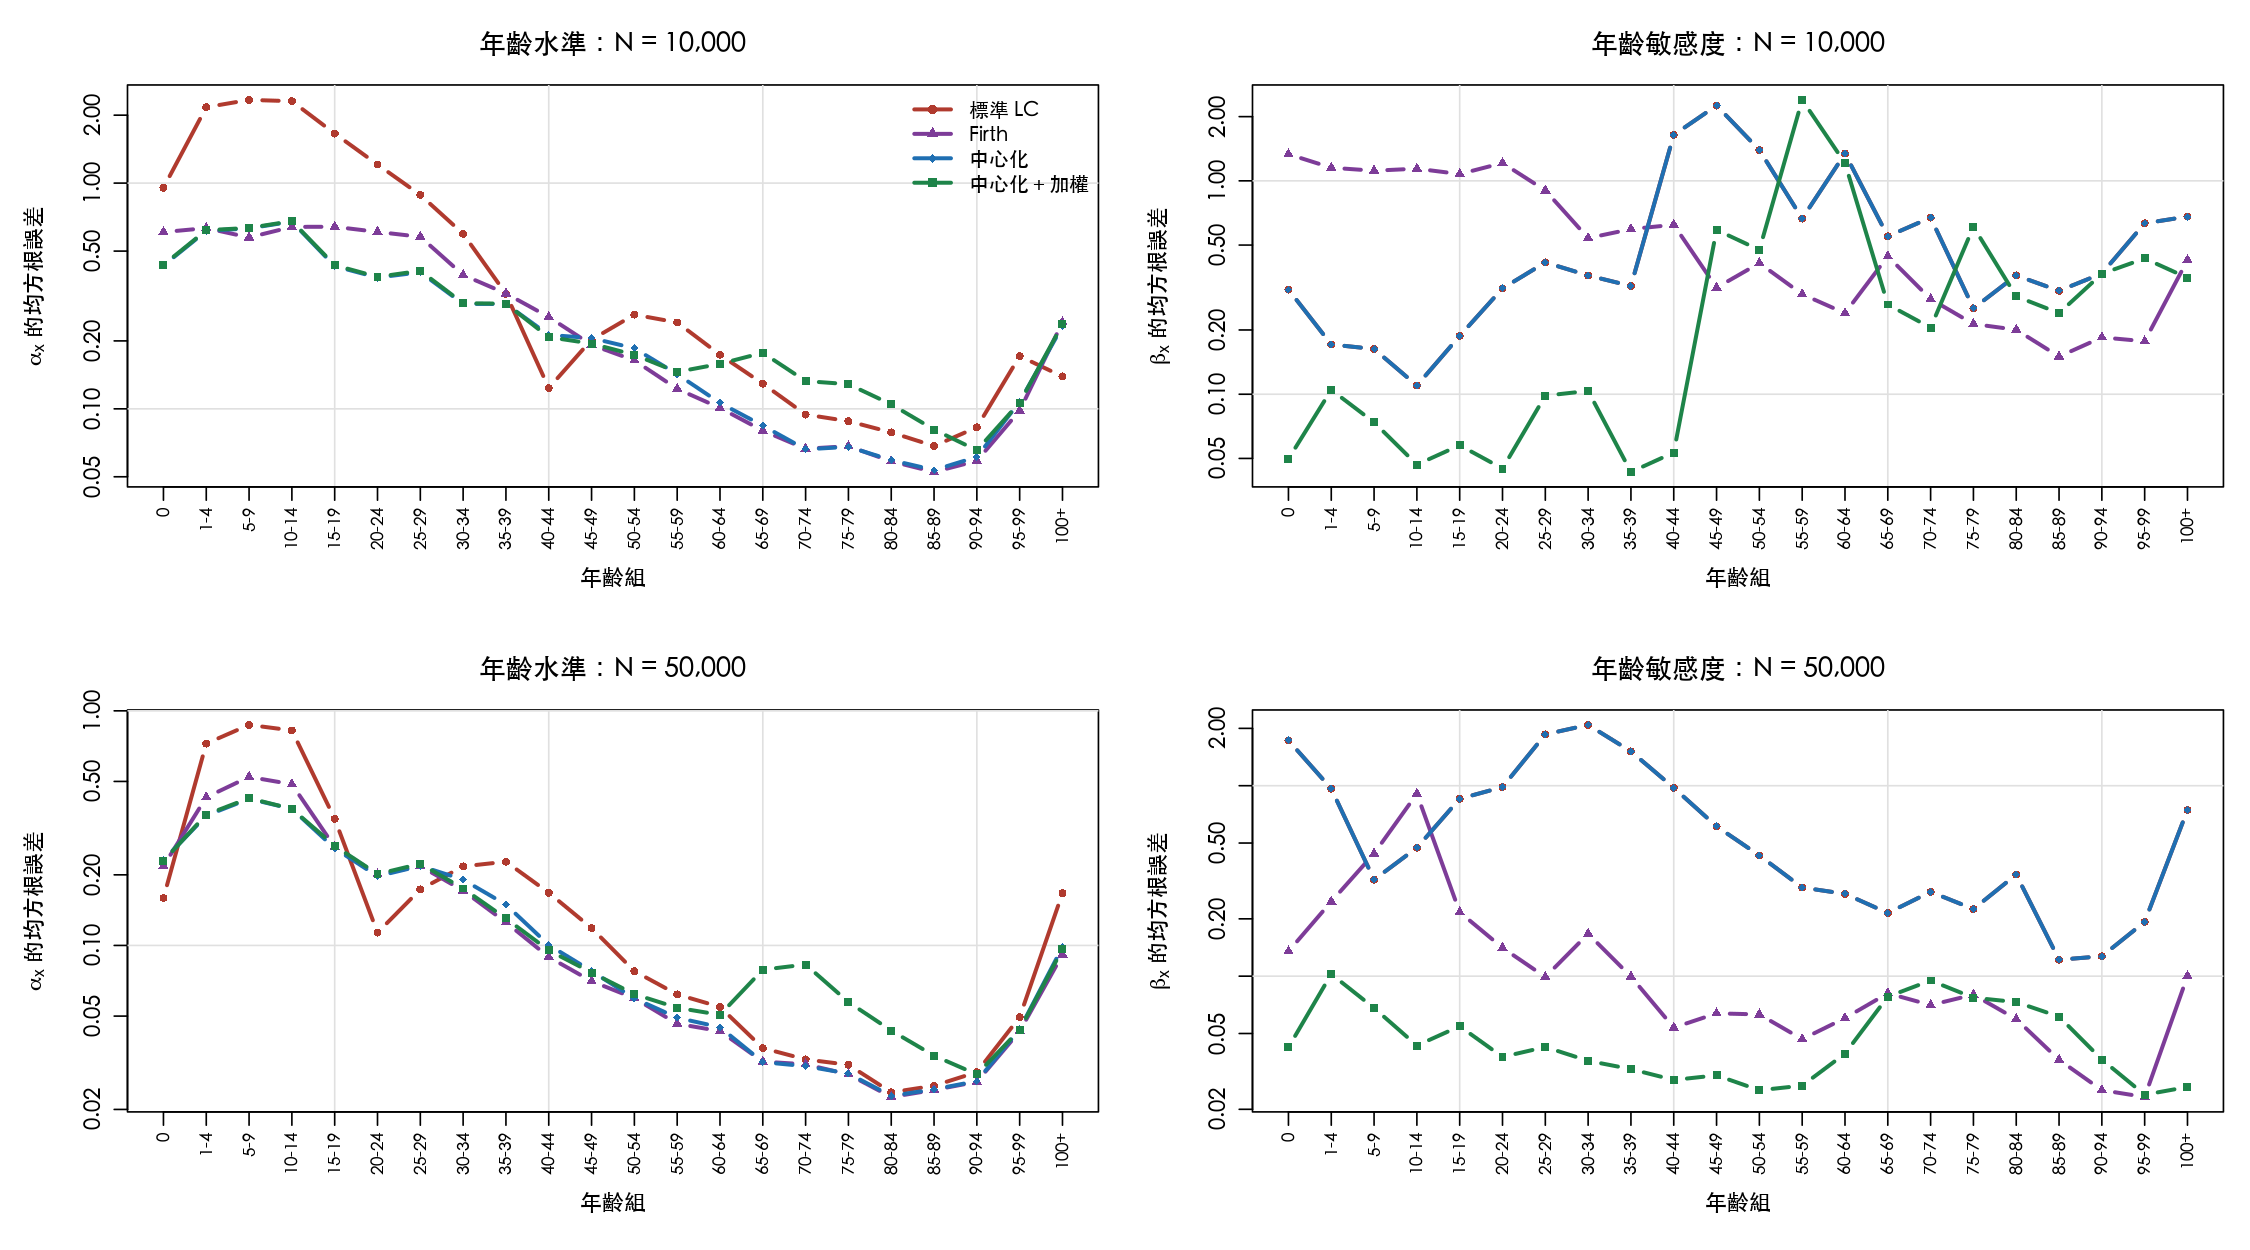
\includegraphics[width=\textwidth]{figT9_age_profile.png}
\caption{逐年齡的均方根誤差（縱軸取對數）。上列為 $N=10^4$、下列為
$N=5\times10^4$；左欄為年齡水準 $\alpha_x$、右欄為年齡敏感度 $\beta_x$。
$\alpha$ 的改善集中在左側死亡數少的年齡，$\beta$ 的改善則遍及全部年齡。
右欄中標準 LC（紅）的線完全被「中心化」（藍）覆蓋，因為僅校正 $\alpha_x$
不改變中心化矩陣，兩者的 $\hat\beta_x$ 逐位相同。}
\label{fig:ageprof}
\end{figure}

表~\ref{tab:ageband} 與圖~\ref{fig:ageprof} 給出四項結果。

第一，$\alpha_x$ 的改善確實集中在死亡數少的年齡，與閉式的預測一致。
人數五萬時 $0$ 至 $14$ 歲組的平均期望死亡數僅 $0.50$ 人，
其 $\alpha$ 的均方根誤差由 $0.645$ 降至 $0.348$，改善近一倍；
而 $60$ 至 $84$ 歲組的平均期望死亡數達 $44$ 人，標準 LC 的誤差本就只有
$0.036$，校正後為 $0.032$，幾無改善空間。
人數一萬時的對比更明顯：$0$ 至 $14$ 歲組由 $1.942$ 降至 $0.588$（$3.3$ 倍），
$15$ 至 $34$ 歲組由 $1.088$ 降至 $0.376$（$2.9$ 倍），
而 $60$ 歲以上兩組的改善倍數皆在 $1$ 附近。
改善的分布與 $b(\mu)$ 的形狀一一對應，這是第\ref{sec:valid}的驗證
在年齡維度上的細部版本。

第二，$\beta_x$ 的改善則遍及全部年齡，且幅度遠大於 $\alpha$。
人數五萬時五個年齡段的改善倍數分別為 $13.6$、$33.9$、$26.7$、$3.7$、$8.0$ 倍。
這與 $\alpha$ 的情形形成明確對比，而兩者的差異正可由第\ref{sec:betadec}的
分解解釋：$\alpha$ 的誤差幾乎全為確定性，故只能由扣除 $b$ 改善，
改善的量即為 $b$ 本身，因而隨年齡而異；
$\beta$ 的誤差九成以上為隨機，其來源是各格變異數的異質，
故由加權處理，而加權對所有年齡同時生效。
須指出的是表中「僅校正 $\alpha$」一欄的 $\beta$ 誤差與標準 LC
\textbf{完全相同}（五個年齡段分別為 $0.8718$、$1.4456$、$0.7645$、
$0.2658$、$0.2970$，與標準 LC 逐位相同），
這在數值上確認了式~\eqref{eq:svd} 的性質：
$\hat\alpha_x$ 在奇異值分解之前定出，事後扣除 $\bar b_x$ 不動中心化矩陣，
因而完全不影響 $\hat\beta_x$。兩項改善可以疊加的理由至此得到逐年齡的驗證。

第三，$15$ 至 $34$ 歲組的 $\alpha$ 沒有改善，而這是可預期的。
該年齡段的平均期望死亡數為 $1.10$，恰落在變號點
$\mu^{\ast}=0.9234$ 附近；由第\ref{sec:method}之四，$b(\mu^{\ast})=0$，
亦即該處本就沒有偏誤可扣。標準 LC 在該段的誤差 $0.213$ 因而幾乎全為變異數，
校正後為 $0.216$，在蒙地卡羅誤差之內。
變號點的位置由閉式事先算出，而實測的「無改善帶」恰好落在該處，
這是閉式的第三項獨立驗證。

第四，$60$ 至 $84$ 歲組在加上資訊加權後反而變差（$0.032\to0.063$），
而這不是中心化造成的。表中「僅校正 $\alpha$」與「＋加權」兩欄的對比顯示，
單純中心化在該段優於標準 LC（$0.0317$ 對 $0.0357$），
加權之後才惡化為 $0.0626$。
原因在於加權版的 $\hat\alpha_x$ 取的是以 $\hat\mu_{x,t}$ 為權重的加權列平均，
而非式~\eqref{eq:svd} 的等權列平均；
在死亡數多、各年變異已經很小的年齡，加權只是把某些年份的觀測放大，
反而引入額外的變異。這指出一個直接的改進方向：
權重應只施加於 $\beta$ 與 $\kappa$ 的求解，而 $\alpha$ 仍取等權列平均；
本文尚未實作該版本，列為後續工作。

\subsection{平均餘命的偏誤與離散}\label{sec:e0var}

前一小節的比較以中位偏誤為主，但偏誤只是估計誤差的一半。
本文的修正只改變估計方程的中心，理論上不應改變其變異數；
這是一個可檢驗的陳述，而檢驗它的地方正是使用者真正關心的標的量。
本小節因此把配適末年零歲平均餘命的 100 次重複分布完整列出，
並一併回答一個相關的問題：死亡率在小人口下的劇烈震盪眾所周知，
平均餘命作為整條死亡率曲線的加權平均，是否也同樣震盪。

\begin{table}[H]
\centering
\caption{零歲平均餘命的偏誤與離散（重複 100 次，單位：歲）}
\small
\renewcommand{\arraystretch}{1.1}
\begin{tabular}{llrrrrrr}
\toprule
$N$ & 估計量 & 中位偏誤 & 標準差 & 四分位距 & 全距 & 均方根誤差 & 命中率\\
\midrule
\multirow{6}{*}{$10^4$}
 & 標準 LC             & $-3.621$ & \textbf{0.945} & \textbf{1.317} & \textbf{4.636} & 3.557 & 0.00\\
 & Poisson MLE          & \textbf{$-0.820$} & 1.155 & 1.438 & 7.646 & \textbf{1.378} & \textbf{0.33}\\
 & Firth               & $-1.327$ & 1.117 & 1.328 & 7.859 & 1.728 & 0.18\\
 & 中心化              & $-1.717$ & 0.880 & 0.985 & 4.232 & 1.775 & 0.08\\
 & 中心化＋加權        & $-1.104$ & 1.639 & 2.368 & 7.671 & 1.915 & 0.17\\
 & 僅校正 $\alpha$＋加權 & $-1.088$ & 1.470 & 2.088 & 7.282 & 1.807 & 0.21\\
\midrule
\multirow{6}{*}{$5\times10^4$}
 & 標準 LC             & $-1.480$ & 0.613 & 0.721 & 3.086 & 1.425 & 0.13\\
 & Poisson MLE          & $-0.202$ & \textbf{0.477} & \textbf{0.683} & \textbf{2.448} & \textbf{0.501} & \textbf{0.67}\\
 & Firth               & $-0.282$ & 0.478 & 0.709 & 2.484 & 0.532 & 0.63\\
 & 中心化              & $-1.522$ & 0.599 & 0.703 & 3.209 & 1.523 & 0.11\\
 & 中心化＋加權        & $+0.023$ & 0.670 & 0.933 & 3.921 & 0.668 & 0.53\\
 & 僅校正 $\alpha$＋加權 & \textbf{$+0.007$} & 0.613 & 0.759 & 3.366 & 0.610 & 0.58\\
\midrule
\multirow{6}{*}{$2\times10^5$}
 & 標準 LC             & $-0.899$ & 0.634 & 0.843 & 3.094 & 1.108 & 0.23\\
 & Poisson MLE          & \textbf{$-0.031$} & 0.276 & 0.378 & 1.463 & \textbf{0.276} & 0.92\\
 & Firth               & $-0.050$ & \textbf{0.275} & \textbf{0.377} & \textbf{1.459} & 0.277 & \textbf{0.93}\\
 & 中心化              & $-1.422$ & 0.693 & 0.943 & 3.018 & 1.415 & 0.14\\
 & 中心化＋加權        & $+0.333$ & 0.344 & 0.409 & 1.984 & 0.504 & 0.65\\
 & 僅校正 $\alpha$＋加權 & $+0.167$ & 0.326 & 0.459 & 1.757 & 0.380 & 0.80\\
\bottomrule
\end{tabular}

\vspace{2pt}
\parbox{0.92\textwidth}{\footnotesize 註：命中率為 100 次重複中
$|\hat e_0-e_0|\le0.5$ 歲的比例。真值為 $84.07$ 歲。}
\label{tab:e0var}
\end{table}

表~\ref{tab:e0var} 的關鍵一列是 $N=5\times10^4$ 的「僅校正 $\alpha$＋加權」。
該列的中位偏誤由標準 LC 的 $-1.480$ 歲降為 $+0.007$ 歲，
而\textbf{標準差完全不變}（$0.613$ 對 $0.613$）。
這正是第\ref{sec:method}之二所推導的內容在標的量上的表現：
式~\eqref{eq:center} 的中心化是在估計方程上加一個\textbf{確定性}的位移，
它改變解的位置而不改變解的隨機波動；
故偏誤被移除，離散保持原狀，均方根誤差隨之由 $1.425$ 降為 $0.610$，
而落在真值正負半歲內的重複比例由 $13\%$ 升至 $58\%$。
本文的修正因此不是以變異數換偏誤的取捨，而是一項沒有代價的位移——
這一點與第\ref{sec:limtable}就正則化所述的「以偏誤換變異數」形成對比，
也說明為何兩者雖都改善估計，性質卻完全不同。

逐格校正的版本則須付代價。「中心化＋加權」把 $b(\hat\mu_{x,t})$ 逐格扣除，
因而把 $\hat\mu$ 的估計誤差注入每一格，標準差由 $0.613$ 升至 $0.670$、
四分位距由 $0.721$ 升至 $0.933$。兩個版本的中位偏誤幾乎相同
（$+0.023$ 對 $+0.007$），差別全在離散，
這再次確認離散的增加來自逐格代入而非中心化本身。

須誠實記下的是 Firth 在這張表上的表現。人數二十萬時 Firth 的均方根誤差為
$0.277$ 歲，優於本文的 $0.380$；人數五萬時為 $0.532$ 對 $0.610$，
亦略優。原因由表直接讀出：Firth 的標準差在兩個規模下分別為 $0.275$ 與
$0.478$，明顯低於本文的 $0.326$ 與 $0.613$。
預先修正在修正偏誤的同時也收縮了估計量，因而連帶降低變異數；
本文的事後扣除則完全不動變異數。兩者的分工因此清楚：
\textbf{若標的是參數本身，本文的修正較佳（見表~\ref{tab:estcmp} 的
SSE($\beta$) 與第\ref{sec:joint}）；若標的是平均餘命且人數在十萬以上，
Firth 的均方根誤差較小}。人數一萬時兩者皆不理想，
Poisson 最大概似的中位偏誤雖最小（$-0.820$），其全距卻達 $7.65$ 歲，
且有 $2\%$ 的重複完全發散，不宜使用。

\begin{table}[H]
\centering
\caption{零歲平均餘命逐年序列的震盪幅度（100 次重複的中位數，單位：歲）}
\small
\begin{tabular}{llrrr}
\toprule
$N$ & 序列 & 逐年變動均值 & 粗糙度 & 全距\\
\midrule
\multirow{4}{*}{$10^4$}
 & 真值                      & 0.299 & 0.330 & 4.534\\
 & 觀測（零格以 $0.5$ 替代） & \textbf{1.304} & \textbf{2.266} & 6.357\\
 & 標準 LC 配適              & 0.866 & 1.440 & \textbf{2.898}\\
 & 中心化＋加權配適          & 1.610 & 2.803 & 8.026\\
\midrule
\multirow{4}{*}{$5\times10^4$}
 & 真值                      & 0.299 & 0.330 & 4.534\\
 & 觀測                      & 0.722 & 1.206 & 5.243\\
 & 標準 LC 配適              & 0.713 & 1.193 & \textbf{2.629}\\
 & 中心化＋加權配適          & 0.815 & 1.402 & 6.601\\
\midrule
\multirow{4}{*}{$2\times10^5$}
 & 真值                      & 0.299 & 0.330 & 4.534\\
 & 觀測                      & 0.453 & 0.702 & 4.759\\
 & 標準 LC 配適              & 0.818 & 1.419 & 3.443\\
 & 中心化＋加權配適          & 0.536 & 0.793 & 6.110\\
\bottomrule
\end{tabular}

\vspace{2pt}
\parbox{0.92\textwidth}{\footnotesize 註：逐年變動均值為
$\frac{1}{T-1}\sum_t|e_0(t+1)-e_0(t)|$；粗糙度為二階差分的平均絕對值
$\frac{1}{T-2}\sum_t|e_0(t+2)-2e_0(t+1)+e_0(t)|$，可濾去線性趨勢而只留
不規則成分；全距為該序列的最大值減最小值，用以判讀趨勢幅度是否被壓縮。}
\label{tab:e0osc}
\end{table}

\begin{figure}[H]
\centering
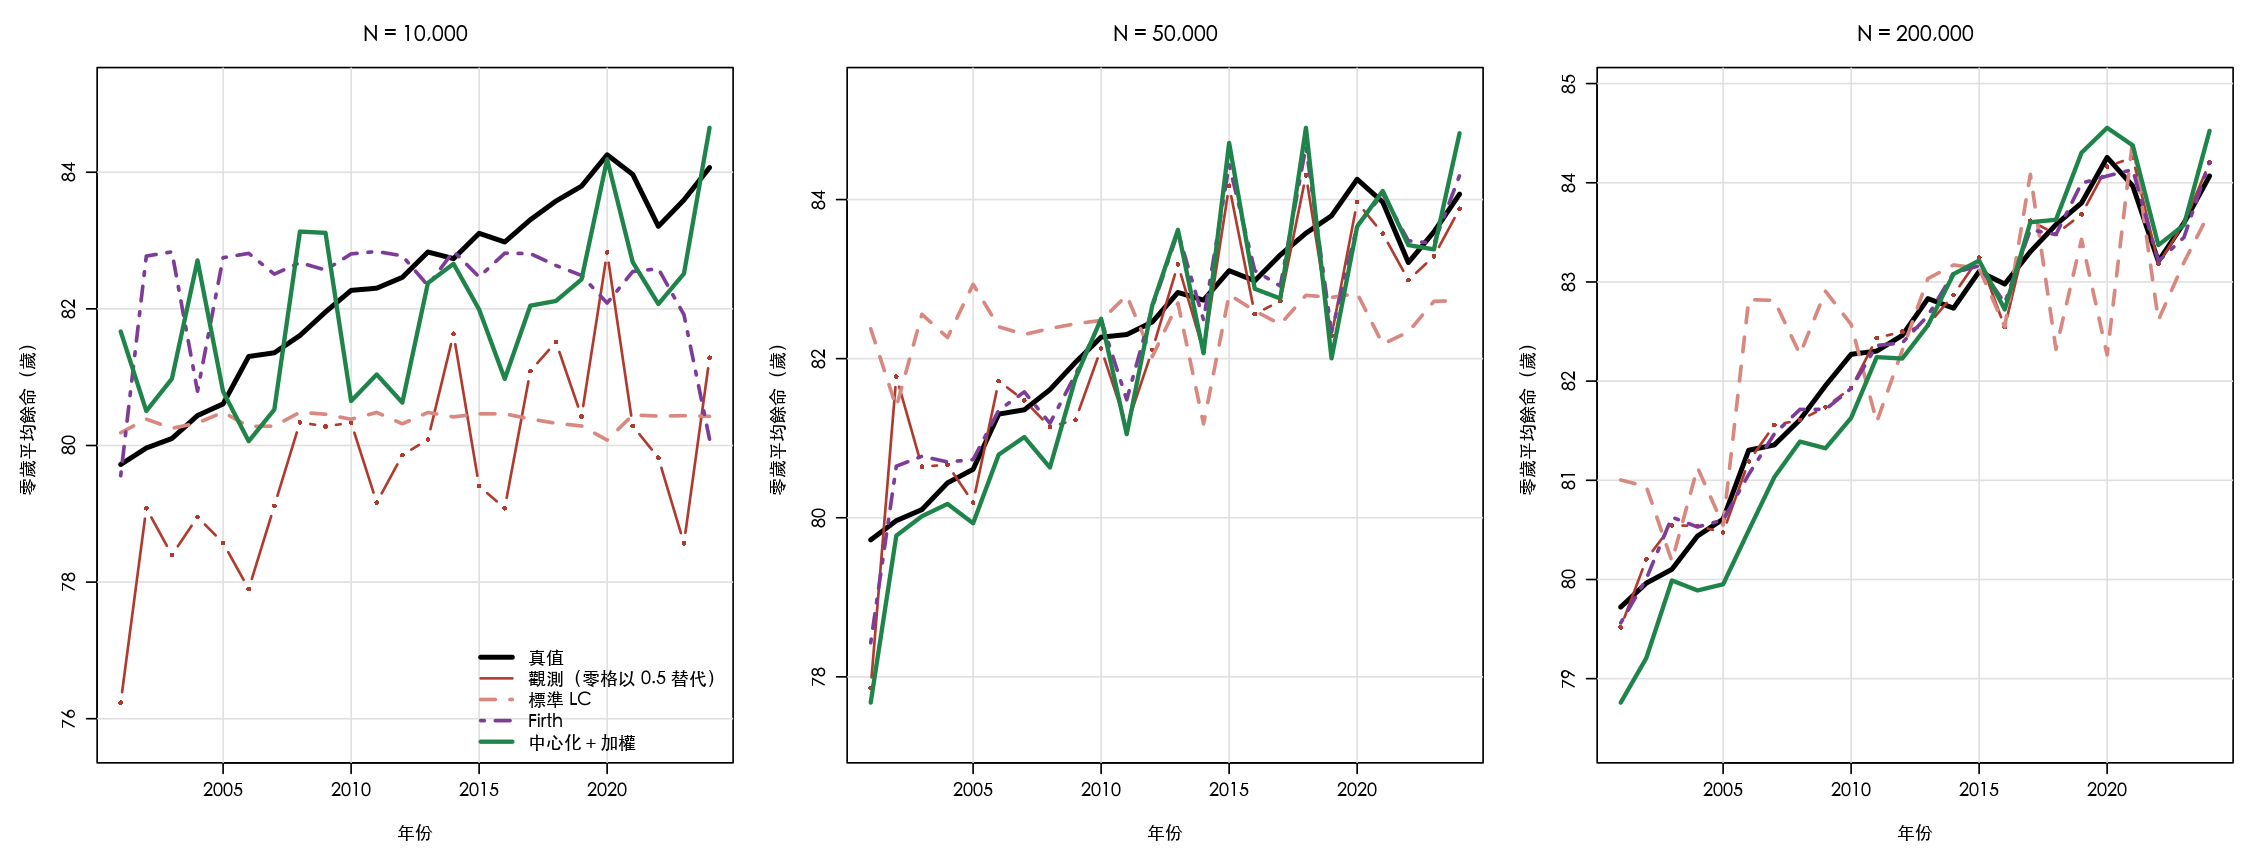
\includegraphics[width=\textwidth]{figT8_e0_oscillation.png}
\caption{零歲平均餘命的逐年序列（單次實現，亂數種子固定）。
觀測序列（深紅）在人數一萬時上下跳動逾兩歲，而真值（黑）平滑遞增；
標準 LC（淺紅虛線）雖把跳動壓下，卻同時把整條趨勢壓平，
其全距僅為真值的六成四。人數二十萬時三條配適線已大致與真值重合。}
\label{fig:e0osc}
\end{figure}

表~\ref{tab:e0osc} 與圖~\ref{fig:e0osc} 回答震盪的問題，
而答案分為兩層。第一層是肯定的：平均餘命確實與死亡率一樣會震盪。
人數一萬時觀測序列的粗糙度為 $2.266$ 歲，為真值 $0.330$ 歲的 $6.9$ 倍；
逐年變動均值為 $1.304$ 歲，亦為真值 $0.299$ 歲的 $4.4$ 倍。
亦即在一個一萬人的地區，相鄰兩年的平均餘命估計值平均相差一歲以上，
而真實的逐年改善不過 $0.3$ 歲——使用者所看到的年度變化，
其中四分之三是雜訊。人數二十萬時該比值降為 $2.1$ 倍，震盪顯著緩解。

第二層則是一個先前未曾注意的現象。把 LC 配適的序列與觀測序列並列，
可以看出LC 並不是把震盪濾掉，而是把震盪換成了趨勢的壓縮。
人數一萬時標準 LC 配適序列的粗糙度為 $1.440$，確實低於觀測的 $2.266$；
但其全距只有 $2.898$ 歲，而真值為 $4.534$ 歲，
亦即二十四年間的改善幅度被壓掉了三成六。
其機制由式~\eqref{eq:astar} 可以理解：秩一結構以 $\hat\kappa_t$ 承載全部
時間訊號，而人數少時 $\hat\kappa_t$ 的訊號雜訊比下降，
奇異值分解所取的第一組奇異向量因而向零收縮。
換言之，第\ref{sec:valid}所刻畫的「震盪看得見而偏誤看不見」，
在時間維度上有一個對應的版本：\textbf{震盪被壓下去了，
但壓下去的同時趨勢也被壓平了，而後者在單一地區的圖上同樣看不出來}。

本文的修正在這一層上沒有改善，甚至更差。中心化加權配適的粗糙度在三個規模
下分別為 $2.803$、$1.402$、$0.793$，皆高於標準 LC 的 $1.440$、$1.193$、
$1.419$；其全距則為 $8.026$、$6.601$、$6.110$ 歲，皆超過真值的 $4.534$，
亦即由壓縮轉為放大。原因在於加權版的 $\hat\kappa_t$ 是由加權奇異值分解的
右奇異向量回推而得，其逐年的回推係數隨各年的權重而變，
使 $\hat\kappa_t$ 的逐年波動被放大。
這是本文修正目前最明確的弱點，也指出下一步的工作：
本文的推導只處理了 $\hat\alpha_x$ 與 $\hat\beta_x$，
而 $\hat\kappa_t$ 的偏誤與波動尚未納入同一個框架。

\subsection{與參考母體修勻法的比較}\label{sec:smr}

第\ref{sec:ref}指出，死亡率文獻另有一條以參考母體壓抑震盪的路，
其代表為 Lee（2003）的 partial SMR。本小節以 Yue et al.（2019, Figure 2）
的七種死亡率比值情境把兩條路並列。

比較的設計如下。小區域的死亡數依第\ref{sec:setup}產生，
其亂數種子只隨人口規模與重複序號變動，故\textbf{七種情境下的小區域資料
完全相同}；三個不使用參考母體的估計量在各情境下的結果因而一致，
可作為橫向比較的基準線。參考母體的人數取 $2\times10^{6}$，
其真實死亡率設為 $m^{R}_{x,t}=m^{0}_{x,t}/s_x$，
其中 $s_x$ 依序取 $0.8$、$1.0$、$1.2$（型態相同）與隨年齡遞增
（$0.5$ 至 $1.5$）、遞減、V 型、倒 V 型（型態不同）；
參考母體的死亡數同樣由 Poisson 產生，故其觀測死亡率亦含抽樣誤差。
除 partial SMR 與 Whittaker 比值修勻外，另加入一個只改動零格處理的估計量
——各格保留觀測死亡率，僅把零格填入 $\mathrm{SMR}_t\cdot m^{R}_{x,t}$
——用以分離「參考母體的貢獻有多少來自零格、有多少來自整條曲線的收縮」。

\begin{table}[H]
\centering
\caption{與參考母體修勻法的比較（$N=5\times10^4$，參考母體 $2\times10^6$，
重複 100 次）}
\small
\renewcommand{\arraystretch}{1.1}
\begin{tabular}{llrrrrr}
\toprule
情境 & 估計量 & $\alpha$ 中位 & $\alpha$ 最大 & SSE($\beta$) & $e_0$ 偏誤 & $e_0$ 標準差\\
\midrule
\multirow{3}{*}{不用參考母體}
 & 標準 LC        & 0.0568 & 0.8658 & 6.7066 & $-1.601$ & 0.610\\
 & Firth          & 0.0077 & 0.1172 & 1.4799 & $-0.171$ & 0.422\\
 & 中心化＋加權   & 0.0223 & 0.0721 & 1.1199 & $+0.003$ & 0.564\\
\midrule
\multirow{3}{*}{$s_x=1.0$（型態相同）}
 & Partial SMR    & \textbf{0.0025} & \textbf{0.0650} & \textbf{0.0486} & $-0.105$ & 0.638\\
 & Whittaker 比值 & 0.0095 & 0.7622 & 6.4063 & $-1.672$ & 0.619\\
 & 零格以 SMR 填補 & 0.0491 & 0.3315 & 1.1273 & $-0.850$ & 0.911\\
\midrule
\multirow{3}{*}{遞增（型態不同）}
 & Partial SMR    & 0.2064 & 0.9033 & 0.0297 & $-1.013$ & 0.569\\
 & Whittaker 比值 & 0.0100 & 0.7531 & 6.9874 & $-1.682$ & 0.672\\
 & 零格以 SMR 填補 & 0.0593 & 0.9098 & 0.7391 & $-1.140$ & 0.869\\
\midrule
\multirow{3}{*}{遞減（型態不同）}
 & Partial SMR    & 0.3313 & 0.7722 & 0.0863 & $+0.613$ & 0.586\\
 & Whittaker 比值 & 0.0123 & 0.7639 & 7.2038 & $-1.649$ & 0.671\\
 & 零格以 SMR 填補 & 0.0318 & 0.2751 & 3.5989 & $-1.033$ & 0.700\\
\bottomrule
\end{tabular}

\vspace{2pt}
\parbox{0.92\textwidth}{\footnotesize 註：$s_x=0.8$ 與 $1.2$ 的結果與
$s_x=1.0$ 幾乎相同（$\alpha$ 最大偏誤 $0.045$ 與 $0.062$），
V 型與倒 V 型則介於遞增與遞減之間，為節省篇幅不另列，
完整結果見 \texttt{tableM1\_smr\_compare.csv}。}
\label{tab:smr}
\end{table}

表~\ref{tab:smr} 給出三項結論。

第一，\textbf{當參考母體的年齡型態與目標區域成固定比例時，
partial SMR 優於本文的修正，且優勢相當大}。
$s_x=1.0$ 時其 $\alpha$ 最大偏誤為 $0.065$、$\mathrm{SSE}(\beta)$ 為 $0.049$，
而本文為 $0.072$ 與 $1.120$；人數一萬時差距更明顯
（$0.064$ 與 $0.046$ 對 $0.611$ 與 $2.968$），
其零歲平均餘命的偏誤甚至只有 $+0.103$ 歲，而本文為 $-1.485$ 歲。
這個結果並不令人意外，但必須明白寫出：
在本節的設計中，參考母體的真實死亡率與目標區域只差一個固定的比例常數，
故 $\mathrm{SMR}\cdot m^{R}_x$ 幾乎就是真值，
而參考母體有兩百萬人、其觀測死亡率的抽樣誤差可忽略。
此一情境是參考母體法最有利的情形，其結果應視為該法的上界，
而非在真實鄉鎮市區應用時可期待的表現。

第二，\textbf{當年齡型態不同時，partial SMR 的 $\alpha$ 偏誤急遽惡化，
而本文的修正不受影響}。遞增與遞減情境下其 $\alpha$ 偏誤中位數為
$0.206$ 與 $0.331$，為本文 $0.022$ 的九倍與十五倍；
零歲平均餘命的偏誤為 $-1.013$ 與 $+0.613$ 歲，
前者甚至劣於未修正的 Firth（$-0.171$ 歲）。
其機制由式~\eqref{eq:psmr} 直接讀出：
$\hat h^2$ 衡量的是兩個母體的整體異質性，而非逐年齡的差異，
故當小區域某些年齡高於、另一些年齡低於參考母體時，
修勻會把兩者一併朝 $\mathrm{SMR}\cdot m^{R}_x$ 拉，使形狀失真。
這與 Yue et al.（2019, Table 1）所報告的現象一致
（該文「遞增」情境的平均絕對百分比誤差由不修勻的 $28.96\%$ 惡化至 $47.65\%$）。
須說明的是，本節的七種情境只改動年齡水準 $\alpha_x$ 而未改動年齡敏感度
$\beta_x$——由 $m^{R}_{x,t}=m^{0}_{x,t}/s_x$ 可知參考母體的 $\beta$ 與
$\kappa$ 與目標區域完全相同——故 partial SMR 在 $\mathrm{SSE}(\beta)$ 上
的優勢是設計使然，不應解讀為該法對 $\beta$ 特別有效。
完整的比較須另設 $\beta_x$ 不同的情境，列為後續工作。

第三，零格的處理方式本身即可解釋偏誤的相當一部分。
只把零格由 $c_0/E$ 改填 $\mathrm{SMR}_t\cdot m^{R}_{x,t}$、其餘各格完全不動，
即使 $\alpha$ 最大偏誤由 $0.866$ 降至 $0.332$、
$\mathrm{SSE}(\beta)$ 由 $6.707$ 降至 $1.127$、
零歲平均餘命的偏誤由 $-1.601$ 歲降至 $-0.850$ 歲；
人數一萬時更由 $2.331$、$9.464$、$-3.753$ 降至 $0.314$、$1.296$、$-0.856$。
\textbf{這直接回答了一個自然的疑問：以標準化死亡比填補零格，
並不會得到與 $c_0=0.5$ 相同的結果，兩者相差約一半的偏誤。}
此一結果同時是對第\ref{sec:method}之二推導的另一項支持——
若偏誤的主要來源確實是零格替代，則只改動零格就應可移除其中相當的部分，
而實測正是如此。剩下的另一半則來自非零格的 Jensen 偏誤
（式~\eqref{eq:jensen}），那一部分只有中心化能處理。

Whittaker 比值修勻在本節的設定下幾無作用，其 $\alpha$ 最大偏誤在人數一萬時
為 $2.302$、與標準 LC 的 $2.331$ 相去無幾。原因是該法在修勻後仍可能給出
非正的死亡率，本文依與標準 LC 一致的慣例把它截在 $c_0/E_{x,t}$，
而在零死亡的年齡該下限恰好生效，使修勻的結果回到零格替代值。
換言之，\textbf{Whittaker 比值修勻並未處理零格問題，
它處理的是非零格的震盪}；這也凸顯了 partial SMR 的真正優勢所在
——它是三者中唯一在零格上提供正值而不需任何慣例的方法。

綜合而言，兩條路徑的取捨可歸結如下：
\textbf{參考母體法以「找得到型態相近的參考母體」為代價換取穩定，
本文的修正以「 Poisson 假設成立」為代價換取穩定}。
前者在參考母體適當時表現更好，但其適當與否無法由目標區域自己的資料判斷；
後者的假設則可由資料檢驗（見第\ref{sec:real}）。
兩者並非互斥：第\ref{sec:disc}將指出，
以參考母體填補零格再施以中心化，是一個自然的結合方向。

\subsection{模型誤設下的穩健性檢驗}\label{sec:real}

前述各小節的模擬取 $D\sim\text{Poisson}(E\,m^{\text{fitted}})$，
亦即假設 LC 模型完全正確，小人口的資料因而不含任何不合模型的結構。
這對檢驗式~\eqref{eq:bform} 本身是恰當的，但無法回答一個實務上更重要的
問題：若真實資料本來就不完全服從秩一雙線性結構，校正是否仍有效？

為此本文另設計一項以真實資料為基礎的檢驗。取實際觀測到的全國死亡數
$D^{\text{obs}}_{x,t}$，以 Poisson 抽薄產生小人口：
\begin{equation}\label{eq:thin}
D_{x,t}\sim\text{Poisson}\big(p\,D^{\text{obs}}_{x,t}\big),\qquad
E_{x,t}=p\,E^{\text{obs}}_{x,t},\qquad p=N/N^{\text{obs}} .
\end{equation}
如此小人口繼承臺灣死亡率真實的逐年不規則性——所有偏離秩一結構的部分
都被保留下來。實測顯示該偏離並非可忽略：
$\log(D^{\text{obs}}/E^{\text{obs}})$ 對全國 LC 配適值的殘差標準差為
$0.0700$。真值仍取全國資料的 LC 配適。

抽薄的方式有兩種可能。二項抽薄
$D\sim\text{Binomial}(D^{\text{obs}},p)$ 與式~\eqref{eq:thin} 的期望值相同，
皆為 $p\,D^{\text{obs}}$，但前者有 $D\le D^{\text{obs}}$ 的上界，
其變異數為 $p(1-p)D^{\text{obs}}$ 而非 $p\,D^{\text{obs}}$。
本文採 Poisson 抽薄，理由是它與式~\eqref{eq:pois} 的分配假設完全一致，
不必另行討論上界與變異數縮減的影響；$p$ 很小時兩者的差異本就可忽略
（本文最大的 $p$ 約為 $0.016$）。

須說明式~\eqref{eq:thin} 打破的是什麼、保留的是什麼。 Poisson 抽薄保持 Poisson 族
（若 $D^{\text{obs}}\sim\text{Poisson}(\mu)$ 則
$D\sim\text{Poisson}(p\mu)$），故式~\eqref{eq:bform} 的形式不變，
只是 $\mu$ 換成 $p\mu$；被打破的不是 Poisson 假設，而是
「$\mu_{x,t}$ 恰好落在秩一雙線性結構上」這個假設。
這正是要檢驗的那一項，因為 $\hat\mu_{x,t}$ 是由 LC 配適算出的，
若真值不在該結構上，$\hat\mu$ 即有系統性誤差，校正也就跟著偏。

\begin{table}[H]
\centering
\caption{真實資料 Poisson 抽薄的結果（重複 100 次，取中位數）}
\small
\begin{tabular}{llrrrrrr}
\toprule
$N$ & 估計量 & $\alpha$ 中位 & $\alpha$ 最大 & SSE($\beta$) & 漂移偏誤 & $e_0$ 偏誤 & $e_0$ 四分位距\\
\midrule
\multirow{5}{*}{\shortstack[l]{$10^4$\\ 零格 216/528}}
 & 標準 LC          & 0.1920 & 2.1676 & 7.719 & 0.2510 & $-2.366$ & 0.965\\
 & Poisson MLE       & 0.0724 & 11.3729 & 14.421 & 0.2487 & \textbf{$-0.553$} & 1.043\\
 & Firth            & \textbf{0.0238} & \textbf{0.1725} & 20.455 & 0.2748 & $-1.131$ & \textbf{0.856}\\
 & 中心化           & 0.0481 & 0.3317 & 13.471 & 0.3289 & $-1.460$ & 0.911\\
 & 中心化 $+$ 加權   & 0.1328 & 0.5953 & \textbf{3.671} & \textbf{0.2315} & $-1.365$ & 1.431\\
\midrule
\multirow{5}{*}{\shortstack[l]{$5\times10^4$\\ 零格 91/528}}
 & 標準 LC          & 0.0896 & 0.7604 & 6.876 & 0.3520 & $-1.366$ & 0.741\\
 & Poisson MLE       & 0.0087 & 0.1175 & 1.655 & \textbf{0.0230} & \textbf{$-0.155$} & 0.545\\
 & Firth            & \textbf{0.0084} & \textbf{0.0895} & 1.437 & 0.0258 & $-0.204$ & 0.547\\
 & 中心化           & 0.0159 & 0.1542 & 6.856 & 0.3407 & $-1.632$ & 0.737\\
 & 中心化 $+$ 加權   & 0.0471 & 0.3306 & \textbf{1.117} & 0.1148 & $+0.393$ & \textbf{0.630}\\
\midrule
\multirow{5}{*}{\shortstack[l]{$2\times10^5$\\ 零格 23/528}}
 & 標準 LC          & 0.0321 & 0.1567 & 1.358 & 0.2139 & $-0.977$ & 1.031\\
 & Poisson MLE       & 0.0063 & 0.0461 & 0.234 & 0.0052 & $+0.024$ & 0.315\\
 & Firth            & \textbf{0.0045} & \textbf{0.0418} & \textbf{0.228} & \textbf{0.0055} & \textbf{$+0.006$} & \textbf{0.314}\\
 & 中心化           & 0.0042 & 0.1541 & 2.873 & 0.2446 & $-1.376$ & 1.183\\
 & 中心化 $+$ 加權   & 0.0347 & 0.3473 & 0.698 & 0.0964 & $+0.640$ & 0.389\\
\bottomrule
\end{tabular}
\label{tab:real}
\end{table}

四項觀察，其中兩項支持本文的推導、兩項則是必須寫下的負面結果。

第一，\textbf{校正在真實資料上仍然有效}。$\alpha$ 最大偏誤在三個規模下
由 $2.1676$、$0.7604$、$0.1567$ 降至 $0.3317$、$0.1542$、$0.1541$，
人數一萬與五萬時分別改善 $6.5$ 與 $4.9$ 倍。
改善幅度與純 Poisson 模擬（$4.7$、$3.6$ 倍）同一量級，
故式~\eqref{eq:bform} 對本資料所含的模型誤設具有一定的穩健性。
理由與前述一致：抽薄不破壞 Poisson 族，而 $\hat\mu$ 只需大致正確即足以把 $b$
算到正確的量級——$b$ 在 $\mu$ 上是平滑的，故 $\hat\mu$ 的中等誤差不會使
$b(\hat\mu)$ 大幅偏離。

第二，$\beta_x$ 的結論不變且更明顯。中心化在三個規模下使
SSE($\beta$) 由 $7.72$、$6.88$、$1.36$ 變為 $13.47$、$6.86$、$2.87$，
即在兩個規模下明顯變差；而中心化加上加權則降至 $3.67$、$1.12$、$0.70$，
三個規模皆優於標準 LC，改善 $2.1$、$6.2$、$1.9$ 倍。
這與第\ref{sec:betadec}表~\ref{tab:betadec} 的分解一致：
$\beta_x$ 的偏誤九成以上是隨機的，須靠加權而非校正。
同一節的另一項觀察是真實資料使標準 LC 的 $\beta$ 更差——
人數五萬時 SSE($\beta$) 在真實抽薄下為 $6.88$、在純 Poisson 模擬下為 $4.45$，
差額來自不合秩一結構的成分也被 $\hat\beta$ 吸收；
相對地加權版本在兩種設計下分別為 $1.12$ 與 $1.02$，幾乎不變。
加權不只處理異質變異，也吸收了一部分模型誤設，
這是純模擬設計所看不到的。

第三，\textbf{在真實資料上 Firth 與 Poisson 最大概似的表現優於本文的修正，
且差距大於純模擬}。人數五萬時 Firth 的 $\alpha$ 最大偏誤為 $0.0895$、
零歲平均餘命偏誤為 $-0.204$ 歲，而中心化加權為 $0.3306$ 與 $+0.393$ 歲；
人數二十萬時差距更大（$0.0418$ 與 $+0.006$ 對 $0.3473$ 與 $+0.640$）。
原因在於本文的校正須代入 $\hat\mu_{x,t}$，而 $\hat\mu$ 是由\textbf{秩一}
配適算出的；真實資料不在秩一結構上，$\hat\mu$ 因而有系統性誤差，
校正跟著偏。 Poisson 最大概似與 Firth 則直接在計數尺度上配適，
不需要先有一個 $\hat\mu$ 的外部估計。
\textbf{這是本文修正最明確的適用界線：它依賴的不只是 Poisson 假設，
還包括秩一結構本身大致正確。}

第四，人數一萬時所有方法都不足以支持編表。
即使最佳的 Poisson 最大概似其零歲平均餘命偏誤仍有 $-0.553$ 歲，
而其 $\alpha$ 最大偏誤達 $11.37$、且有 $2\%$ 的重複發散；
Firth 雖穩定，偏誤仍有 $-1.131$ 歲。
在 528 格中有 $216$ 格為零的情形下，資訊量本身已不足，
任何估計量都只能在偏誤與變異之間重新分配，而無法同時降低兩者。

\subsection{兩參數的聯合改善}\label{sec:joint}

表~\ref{tab:estcmp} 呈現了一個表面上的取捨：逐格校正把 $\alpha$ 修好卻把
$\beta$ 弄差，加上加權後 $\beta$ 修好了但 $\alpha$ 又退了一些。
這是否表示兩者只能擇一？第\ref{sec:betadec}的分解說不是，而且指出了出路。

由 Proposition~\ref{prop:beta}，逐格扣除 $b$ 同時做了兩件事：一是移除
$\alpha_x$ 的偏誤，其量為列平均 $\bar b_x$；二是移除 $\beta_x$ 的確定性
擾動 $\Delta_{x,t}=b(\mu_{x,t})-\bar b_x$。但表~\ref{tab:betadec} 已顯示
第二件事的收益很小——$\Delta$ 只佔 $\beta$ 總誤差的一成以下——
而逐格扣除所注入的 $\hat\mu$ 噪音卻進入每一格，對依賴跨格相對大小的
$\beta$ 傷害甚大。既然如此，正確的設計是只做第一件事：
把 $\hat\alpha_x$ 扣掉 $\bar b_x$，而完全不動中心化矩陣。
由式~\eqref{eq:svd}，$\hat\alpha_x$ 是列平均、在奇異值分解之前即已定出，
故事後扣除 $\bar b_x$ 對 $\hat\beta_x$ 與 $\hat\kappa_t$ 的計算毫無影響；
兩項改善因而可以疊加而不互相干擾。表~\ref{tab:joint} 檢驗此一設計。

\begin{table}[H]
\centering
\caption{逐格校正與僅校正 $\alpha$ 的比較（$N=5\times10^4$，重複 100 次）}
\small
\begin{tabular}{lrrrrr}
\toprule
估計量 & $\alpha$ 中位 & $\alpha$ 最大 & SSE($\beta$) & 漂移偏誤 & $e_0$ 偏誤（歲）\\
\midrule
標準 LC              & 0.0611 & 0.8658 & 4.4494 & 0.3339 & $-1.480$\\
Firth                & 0.0088 & 0.0680 & 1.4102 & \textbf{0.0485} & $-0.282$\\
逐格校正             & 0.0093 & 0.2434 & 8.8335 & 0.3335 & $-1.522$\\
逐格校正 $+$ 加權     & 0.0110 & 0.2524 & \textbf{1.0230} & 0.1381 & $+0.023$\\
僅校正 $\alpha$      & \textbf{0.0063} & \textbf{0.0439} & 4.4494 & 0.3339 & $-1.466$\\
僅校正 $\alpha$ $+$ 加權 & 0.0238 & 0.0715 & 1.1497 & 0.1407 & \textbf{$+0.007$}\\
\bottomrule
\end{tabular}
\label{tab:joint}
\end{table}

結果證實了上述推理，而且有兩處值得特別指出。其一，僅校正 $\alpha$ 的版本
其 SSE($\beta$) 為 $4.4494$，與標準 LC \textbf{完全相同到小數第四位}——
這不是巧合，而是因為該作法根本沒有碰到中心化矩陣，$\hat\beta$ 的計算
逐位元一致。其二，該版本的 $\alpha$ 最大偏誤為 $0.0439$，\textbf{優於
Firth 的 $0.0680$}，是全表最低；相對地逐格校正為 $0.2434$，
可見逐格扣除所注入的噪音同時也傷害了 $\alpha$ 本身。
把它與資訊加權疊加之後，$\alpha$ 最大偏誤 $0.0715$ 與 Firth 相當、
SSE($\beta$) $1.1497$ 亦與 Firth 的 $1.4102$ 相當，
而零歲平均餘命的偏誤為 $+0.007$ 歲，是全表最接近零者。
因此兩者可以同時改善，條件是校正只施加在它該施加的地方。

圖~\ref{fig:pareto} 把這件事畫成一張取捨圖，橫軸為 SSE($\beta$)、
縱軸為 $\alpha$ 最大偏誤，皆取對數，愈靠左下愈好。

\begin{figure}[H]
\centering
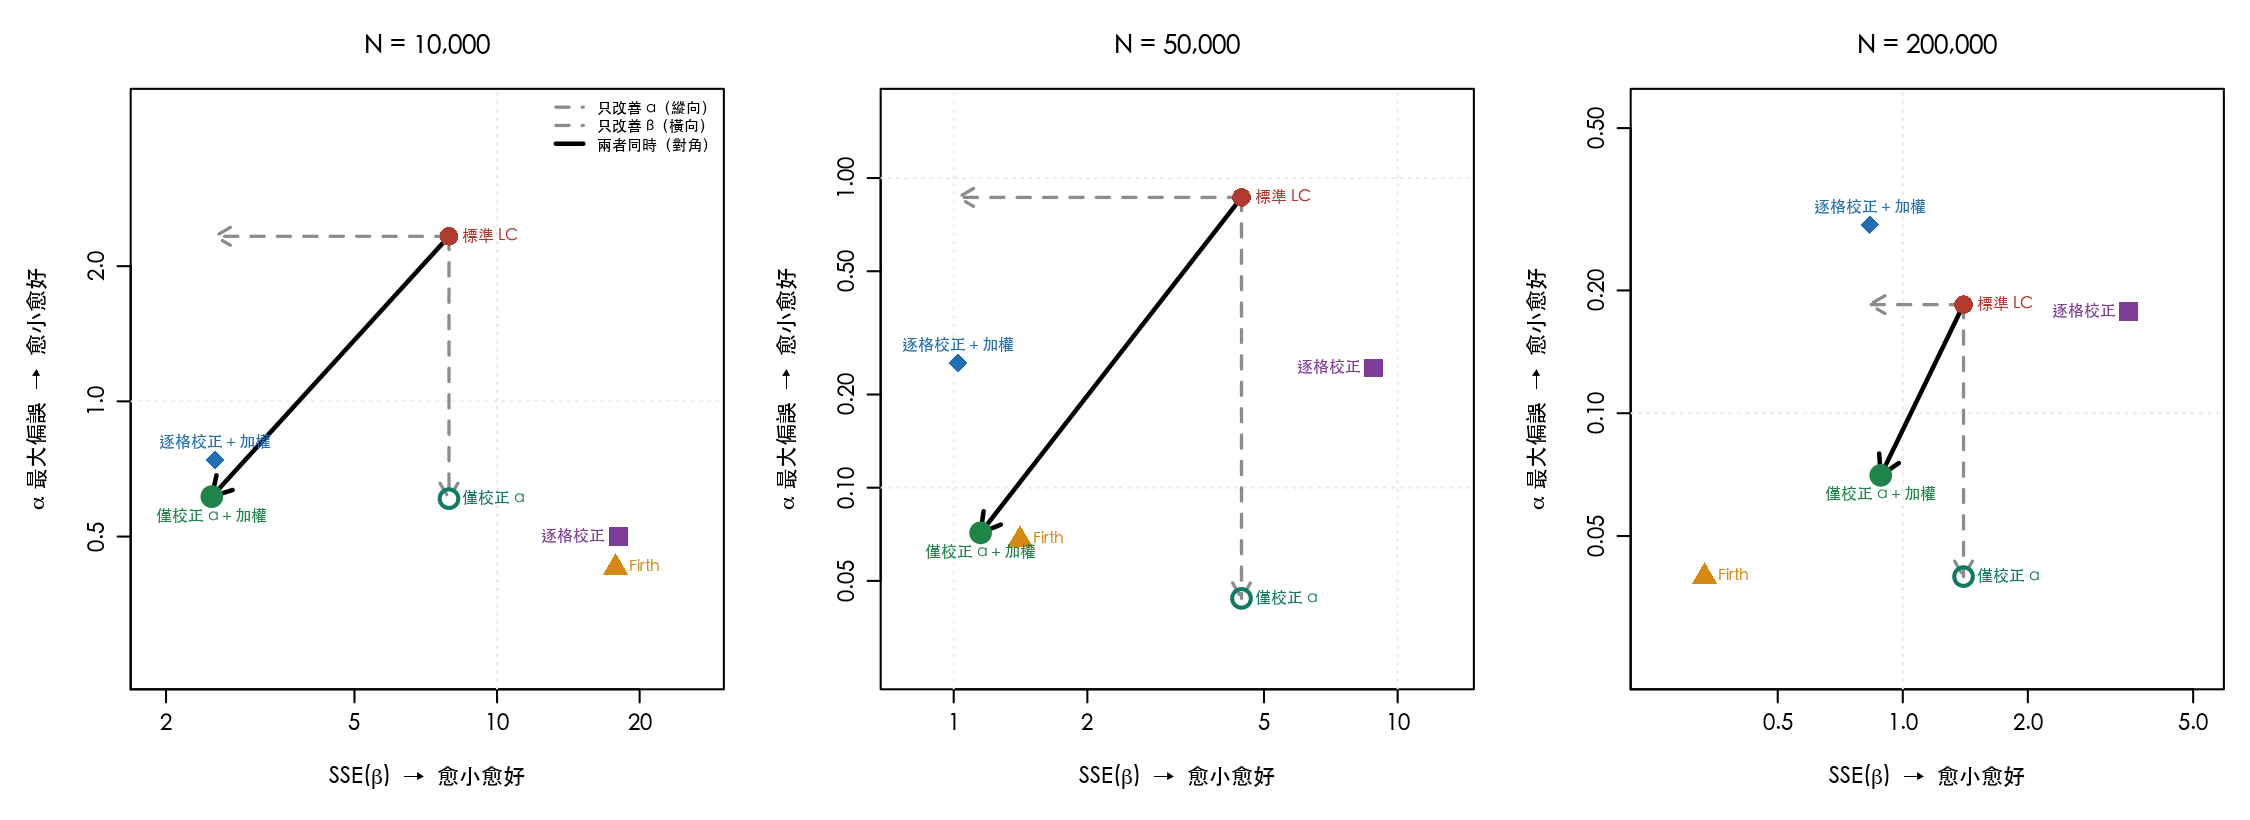
\includegraphics[width=\textwidth]{figT6_pareto.png}
\caption{$\alpha$ 與 $\beta$ 的取捨圖。由標準 LC 出發，僅校正 $\alpha$ 是
\textbf{垂直向下}（只改善 $\alpha$，$\beta$ 完全不動）、逐格校正加權是
\textbf{水平向左}（主要改善 $\beta$），而僅校正 $\alpha$ 加上加權則是
\textbf{對角線}（兩者同時）。$N=5\times10^4$ 時該點與 Firth 幾乎重合。}
\label{fig:pareto}
\end{figure}

圖~\ref{fig:pareto} 的三個箭頭是本小節的摘要。垂直的虛線箭頭表示僅校正
$\alpha$ 只在縱軸上移動，橫軸位置分毫未變；水平的虛線箭頭表示加權主要在
橫軸上移動；而實線的對角箭頭表示兩者疊加後同時往左下走。
人數二十萬時 Firth 仍在更左下的位置，但在五萬與一萬時兩者已相當接近，
而後者正是鄉鎮市區的實際規模。

圖~\ref{fig:jointband} 則把同一件事回到逐年齡的層次。

\begin{figure}[H]
\centering
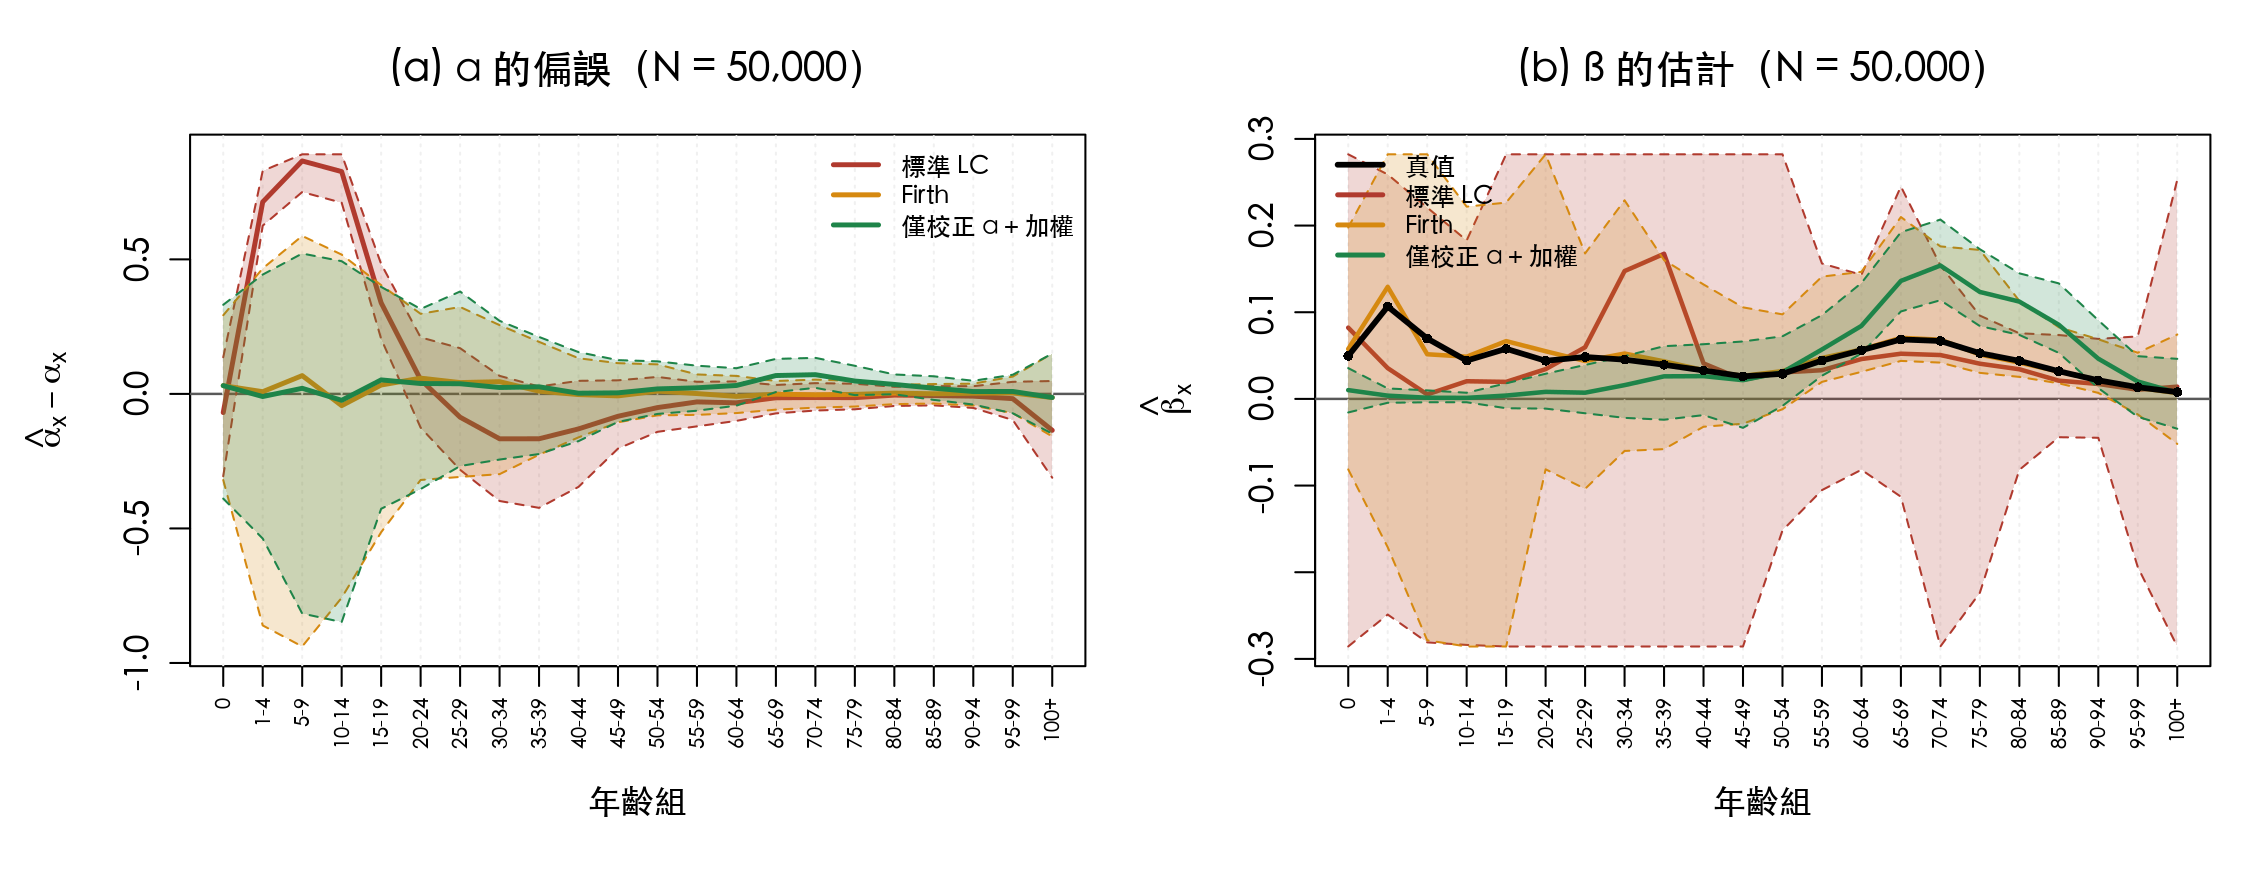
\includegraphics[width=\textwidth]{figT7_joint_band.png}
\caption{標準 LC、Firth 與僅校正 $\alpha$ 加權三者的逐年齡分布
（$N=5\times10^4$，5--95\% 帶）。(a) 綠線在全年齡貼近零，
標準 LC 則在幼年組隆起；(b) 綠色的帶最窄，其中線在多數年齡跟上真值。}
\label{fig:jointband}
\end{figure}

\subsection{本文修正的限制}\label{sec:lim}

本節把前述各小節所顯露的限制集中陳述，每一項都可回到第\ref{sec:limtable}
所列的某一項，而其中三項是前一版報告尚未記錄的。

第一項是純中心化使 $\beta$ 變差：表~\ref{tab:estcmp} 中其 SSE($\beta$)
為 $18.05$、$8.83$、$3.50$，均大於標準 LC 的 $7.92$、$4.45$、$1.40$。
機制是逐格扣除 $b(\hat\mu_{x,t})$ 把 $\hat\mu$ 的估計誤差注入每一格，
而 $\beta$ 的估計依賴跨格的相對大小，因而對這種注入特別敏感，
必須配合加權才能抵銷。這是真實的代價而非實作問題，
也正是第\ref{sec:limtable}就正則化所載「以偏誤換變異數」的另一面：
此處交換的方向相反，是以變異數換偏誤，而在 $\beta$ 上此一交換並不有利。

第二項是 Firth 在 $\alpha$ 最大偏誤與平均餘命的均方根誤差上仍有優勢。
就 $\alpha$ 最大偏誤而言，其 $0.4267$、$0.0680$、$0.0398$ 優於逐格中心化的
$0.5008$、$0.2434$、$0.1778$；就平均餘命而言，表~\ref{tab:e0var} 顯示
Firth 的均方根誤差在人數五萬與二十萬時為 $0.532$ 與 $0.277$ 歲，
優於本文的 $0.610$ 與 $0.380$ 歲，其來源是較小的變異數
（$0.478$ 與 $0.275$ 對 $0.613$ 與 $0.326$）。
理由與兩者的方法性質一致：中心化只移除期望值的偏移，每一次實現的偏差仍在，
且不改變變異數；Firth 則在計數尺度上估計，在修正偏誤的同時也收縮了估計量。
這對應第\ref{sec:limtable}就預先修正所述的優點，也說明事後與預先兩路並非
等價。本文另掃描了部分扣除（係數 $0.8$ 與 $0.6$），結果一律較完全扣除為差，
故不存在過度校正，原先「$\hat\mu$ 有誤差故應保守扣除」的推測不成立。

第三項與第\ref{sec:weight}的推導有關：該節所導出的最適權重
式~\eqref{eq:woptmu} 雖然正確，實測上卻與簡單的冪次權重沒有可分辨的差異。
以 $\sqrt{\hat\mu}$、$\hat\mu$ 與式~\eqref{eq:woptmu} 三者相比，
$N=2\times10^5$、$c=1.345$ 時 $\beta$ 的平方誤差和分別為 $0.4051$、
$0.4108$、$0.4017$，彼此的差距皆在蒙地卡羅誤差之內；
而同一設定下無加權為 $1.0100$。換言之真正有價值的是「有沒有加權」，
而非「權重的形式對不對」。解釋是目標函數對權重的冪次相當平坦：
權重的作用是反映 $\sigma_x^2$ 跨三個數量級的落差，三者都足以做到這件事，
其間的差異屬二階。實務上因此取最簡單的 $w=\hat\mu$ 即可，
而式~\eqref{eq:woptmu} 的價值在於它說明了為何固定冪次原則上不可能最適
——這一點在推導上重要，在本資料的量級下則不重要。

第四項是本次新增的檢驗所顯露的：\textbf{本文的修正不只依賴 Poisson 假設，
也依賴秩一結構本身大致正確}。第\ref{sec:real}的 Poisson 抽薄顯示，
當資料保留臺灣死亡率真實的不規則性時，中心化加權在人數五萬與二十萬時的
平均餘命偏誤為 $+0.393$ 與 $+0.640$ 歲，而 Firth 為 $-0.204$ 與 $+0.006$ 歲。
原因是 $b(\hat\mu_{x,t})$ 須代入由秩一配適算出的 $\hat\mu$，
而真實資料不在秩一結構上時 $\hat\mu$ 即有系統性誤差。
這項限制在純 Poisson 模擬中完全看不到，因為該設計使資料恰好落在秩一結構上。

第五項是資訊加權在死亡數多的年齡反而有害。
表~\ref{tab:ageband} 顯示人數五萬時 $60$ 至 $84$ 歲組的 $\alpha$ 均方根誤差，
單純中心化為 $0.0317$（優於標準 LC 的 $0.0357$），加權後則惡化為 $0.0626$。
原因是加權版的 $\hat\alpha_x$ 取加權列平均而非等權列平均，
在各年變異本已很小的年齡只是引入額外的變異。
一個直接的改進是讓權重只作用於 $\beta$ 與 $\kappa$ 的求解，
而 $\alpha$ 維持等權列平均；本文尚未實作此版本。

第六項是時間參數 $\kappa_t$ 完全未納入本文的框架，而其後果已可觀察到。
表~\ref{tab:e0osc} 顯示中心化加權所配適的平均餘命序列，其粗糙度在三個規模
下皆高於標準 LC，全距亦由標準 LC 的壓縮轉為放大。
本文的推導只處理 $\hat\alpha_x$ 的 Fisher 不一致與 $\hat\beta_x$ 的擾動分解，
$\hat\kappa_t$ 的偏誤與逐年波動尚無對應的刻畫；
在死亡率預測的應用中這一項至關重要，是本文最優先的後續工作。

第七項是人數一萬以下時所有方法都不足以支持編表。
表~\ref{tab:e0var} 中該規模下最佳的均方根誤差為 $1.378$ 歲，
而第\ref{sec:popstr}顯示在年輕的人口結構下本文的修正甚至劣於標準 LC，
原因是該處的 $\hat\mu$ 本身已無資訊可用，
\textbf{校正在最需要它的時候自動失效}。

\section{討論與結論}\label{sec:disc}

本文由 $M$-估計、混合模型與 M-分位數 LASSO 三條一般理論的性質，
推導小人口 LC 模型的偏誤，得到三項結論。

第一，既有文獻以模擬觀察到的 $\alpha_x$ 偏誤，在 $M$-估計的架構中有一個
明確的名字與一個閉式：它是標準 LC 估計方程的\textbf{Fisher 不一致}，
其量為 $b(\mu;c_0)$（Proposition~\ref{prop:fisher}），而 $\hat\alpha_x$ 的偏誤
恰為各格 $b$ 的算術平均（Corollary~\ref{cor:alpha}），且後者是恆等式。
臺灣資料的驗證給出 $1.000$、$1.000$、$0.988$ 的相關係數。
這把「偏誤有多大」由一個須以模擬回答的問題，變成一個可以計算的量。

第二，混合模型的表示式說明了零格替代在統計上是什麼，並給出兩個門檻。
式~\eqref{eq:mix} 顯示每一格是一個混合權重\textbf{已知}的兩成分混合，
因此古典穩健統計為未知污染比例所付的效率代價在此不必付——
這是本文選擇中心化而非穩健損失的理由。而把崩潰點理論代入該表示式，
即得中位數失效的解析門檻 $\mu<\ln2$（式~\eqref{eq:ln2}），
與偏誤變號的門檻 $\mu^\ast=0.9234$ 恰成對比：前者是資料的性質，
後者則隨分析者選定的 $c_0$ 移動。

第三，M-分位數 LASSO 的分類說明中心化與既有補救的關係是正交的，
並給出兩項獲得證實的預測：中心化大幅改善 $\alpha_x$，但不改善
$\beta_x$ 與漂移項。後者本身即是結果——它證明小人口 LC 的偏誤
至少來自兩個獨立機制，$\alpha_x$ 源於估計方程的中心不正，
$\beta_x$ 源於權重不當。

第四，\textbf{就「能不能在某些假設下降低 $\alpha_x$ 與 $\beta_x$ 的小樣本
偏誤」這個問題，本文的答案對兩個參數不同，且差別可以量化。}
第\ref{sec:betadec}把兩者的偏誤精確分解為確定性與隨機成分：
$\alpha_x$ 的偏誤在人數一萬與五萬時有 $100\%$ 與 $97\%$ 是確定性的，
故在 Poisson 假設下可由閉式近乎完全移除；$\beta_x$ 的偏誤則只有
$9.2\%$ 與 $5.8\%$ 是確定性的，其餘來自異質變異噪音旋轉主奇異向量，
無論把 $b$ 算得多準都無法處理，須改以加權為之。
因此可降低偏誤的條件是兩個而非一個： Poisson 假設足以處理 $\alpha_x$，
「加權後噪音變異數大致相等」則足以處理 $\beta_x$，而後者不由本文的閉式提供。

第五，以真實資料 Poisson 抽薄的檢驗顯示上述結論對模型誤設具有一定的穩健性
（第\ref{sec:real}）。$\alpha$ 最大偏誤的改善幅度在真實抽薄與純 Poisson 模擬
下同為 $1.2$ 至 $6.5$ 倍的量級。一項只有真實資料才顯示出來的發現是：
標準 LC 的 SSE($\beta$) 在真實抽薄下較純模擬明顯為差（人數五萬時 $6.88$
對 $4.45$），而加權版本在兩種設計下幾乎不變（$1.12$ 對 $1.02$），
亦即加權不只處理異質變異，也吸收了一部分模型誤設。
但同一節也顯示本文修正的一項界線：真實資料不落在秩一結構上時，
$\hat\mu$ 本身即有系統性誤差，使校正在人數五萬以上時的平均餘命偏誤劣於
Firth。

第六，偏誤不只隨人口規模而變，也隨人口的年齡結構而變，而閉式對兩者
一併給出解釋（第\ref{sec:popstr}）。在總人數固定於五萬的條件下，
把年齡結構由 2001 年的全國結構（$65$ 歲以上占 $8.5\%$）換成老化的結構
（$31.7\%$），標準 LC 的 $\alpha$ 最大偏誤由 $0.428$ 升至 $1.456$、
零歲平均餘命的偏誤由 $-1.055$ 歲擴大至 $-2.109$ 歲，
其惡化幅度與把人數由五萬降到一萬相當。閉式在三種結構下預測逐年齡偏誤的
相關係數皆在 $0.998$ 以上、迴歸斜率皆在 $0.96$ 至 $1.00$ 之間，
而校正後三種結構的平均餘命偏誤落在 $-0.235$ 至 $+0.066$ 歲之內。
\textbf{這對使用者有直接的意義：分析者只要有曝露數與一組初步的死亡率估計，
就可以在不做任何模擬的情形下事先算出該地區的 LC 估計會偏多少，
而人口老化嚴重的鄉鎮市區需要更謹慎地處理。}

第七，偏誤的移除沒有以變異數為代價，這一點可由平均餘命的分布直接讀出
（第\ref{sec:e0var}）。人數五萬時「僅校正 $\alpha$＋加權」使中位偏誤由
$-1.480$ 歲降為 $+0.007$ 歲，而一百次重複的標準差維持在 $0.613$ 歲不變，
均方根誤差因而由 $1.425$ 降為 $0.610$ 歲。
這與中心化的性質一致：它在估計方程上加一個確定性的位移，改變解的位置
而不改變解的隨機波動。相對地，逐格施加的版本因代入 $\hat\mu$ 而使標準差
由 $0.613$ 升至 $0.670$，兩版本的中位偏誤卻幾乎相同，
再次確認離散的增加來自逐格代入而非中心化本身。
同一節另發現平均餘命確實與死亡率一樣會震盪——人數一萬時觀測序列的
二階差分平均絕對值為真值的 $6.9$ 倍——
但 LC 配適並不是把震盪濾掉，而是把震盪換成趨勢的壓縮：
其配適序列二十四年間的全距只有真值的六成四。

第八，與 Lee（2003）的 partial SMR 修勻比較後，兩條路的取捨得以量化
（第\ref{sec:smr}）。當參考母體的年齡型態與目標區域成固定比例時，
partial SMR 全面優於本文的修正（人數五萬時 $\alpha$ 最大偏誤 $0.065$
對 $0.072$、$\mathrm{SSE}(\beta)$ $0.049$ 對 $1.120$）；
但當型態不同時其 $\alpha$ 偏誤中位數惡化至本文的九至十五倍，
零歲平均餘命的偏誤達 $-1.013$ 與 $+0.613$ 歲。
\textbf{參考母體法以「找得到型態相近的參考母體」為代價換取穩定，
本文的修正以「 Poisson 假設與秩一結構成立」為代價換取穩定；
前者的前提無法由目標區域自己的資料判斷，後者則可以。}
該節另發現只把零格改以標準化死亡比填補、其餘各格完全不動，
即可使人數五萬時的平均餘命偏誤由 $-1.601$ 歲降至 $-0.850$ 歲，
人數一萬時由 $-3.753$ 歲降至 $-0.856$ 歲。
這直接回答了一個自然的疑問：以標準化死亡比填補零格並不會得到與
$c_0=0.5$ 相同的結果，兩者相差約一半的偏誤；
同時也再次支持「偏誤的主要來源是零格替代」這個推導結論。

把第\ref{sec:limtable}所列的各項限制逐一回顧，可以看出本文的結果如何落在
既有文獻所記載的限制之中。事後修正所載「須最大概似估計值存在」這項限制，
在本問題上確實出現且後果嚴重——Poisson 最大概似在人數一萬時給出 $-13.03$，
而本文由邊際分布推導的作法正是為繞過它而設。
預先修正的限制（$O(n^{-1})$ 的漸近性）同樣出現，Firth 的殘餘偏誤
在人數一萬時仍有 $0.427$，只是遠小於未修正的量級。
穩健損失的兩項限制則一項被繞過、一項被證實：效率代價因污染比例已知
而不必承受，但「污染為少數」的前提在幼年組明確不成立，其比例達 $0.74$，
超過崩潰點所允許的 $50\%$。
正則化的調參限制在本問題上格外嚴重，因為 LC 的跨格借力使交叉驗證無合法的
切分方式；而「以偏誤換變異數」的取捨則以另一種形式出現在圖~\ref{fig:bband}
上——加權使 $\beta$ 的帶寬收窄七倍，卻使中線偏離真值。
經驗貝氏收縮的「直接估計量不偏」前提亦不完全成立，
因 $\hat\beta_x$ 本身即含 $9.2\%$ 的確定性偏誤。
混合模型的限制（成分須有密度）使 EM 無從施加，但因 $\pi$ 已知而不構成障礙。
參考母體修勻的限制則在第\ref{sec:smr}得到定量的確認。

後續工作有六項，依優先序排列。
第一是把 $\hat\kappa_t$ 納入同一個框架。本文的推導只處理 $\hat\alpha_x$ 的
Fisher 不一致與 $\hat\beta_x$ 的擾動分解，而第\ref{sec:e0var}顯示修正後的
$\hat\kappa_t$ 路徑反而更不平滑；在死亡率預測的應用中這一項至關重要。
第二是 $\hat\beta_x$ 的偏誤閉式。$\hat\beta_x$ 與 $\hat\kappa_t$ 為奇異向量，
其偏誤須以逐元的矩陣擾動理論處理，而非以子空間的角度界限處理。
第三是把參考母體與本文的修正結合。第\ref{sec:smr}顯示兩者分別處理零格與
非零格的偏誤，以 $\mathrm{SMR}\cdot m^{R}_x$ 填補零格再施以中心化，
是一個自然且可立即檢驗的組合；此即 0929 討論中所提的問題。
第四是分配假設的放寬。式~\eqref{eq:bform} 依賴 Poisson 假設，
實際死亡數若過度離散（例如同一機構的死亡具相關性），
式~\eqref{eq:jensen} 的一階項應為 $-\sigma_D^2/(2\mu^2)$ 而非 $-1/(2\mu)$，
負二項假設下的對應閉式可同法寫出但尚未做。
第五是比較設計的補全。第\ref{sec:smr}的七種情境只改動年齡水準 $\alpha_x$
而未改動年齡敏感度 $\beta_x$，故 partial SMR 在 $\mathrm{SSE}(\beta)$ 上的
優勢是設計使然；完整的比較須另設 $\beta_x$ 不同的情境。
第六是真實的鄉鎮市區資料。本文以全國配適為真值作模擬，
並以 Poisson 抽薄檢驗模型誤設，但尚未在真實的小區域資料上驗證，
而該驗證是本方法能否用於編製鄉鎮市區生命表的最後一步。

\section*{參考文獻}
\addcontentsline{toc}{section}{參考文獻}

\noindent\textbf{一、中文部分}
\begin{itemize}[leftmargin=2em, label={}, itemsep=3pt]
  \item[] 王信忠、金碩、余清祥（2012）。小區域死亡率推估之研究。人口學刊，
        45：121-154。
  \item[] 王信忠、余清祥、王子瑜（2017）。臺灣原住民死亡率暨生命表編撰研究。
        人口學刊，55：99-131。
  \item[] 余清祥、王信忠、陳譽騰（2021）。年輪變動比用於小區域人口推估的探討。
        人口學刊，63：99-133。
  \item[] 余清祥、王信忠、呂靖翎（2025）。平均餘命與標準化死亡率之相關分析。
        人口學刊，85-116。
  \item[] 陳政勳、余清祥（2010）。小區域人口推估研究：臺北市、雲嘉兩縣、
        澎湖縣的實證分析。人口學刊，41：153-183。
\end{itemize}

\vspace{6pt}
\noindent\textbf{二、英文部分}
\begin{itemize}[leftmargin=2em, itemsep=2pt, parsep=0pt]
  \item[] Albert, A., and Anderson, J. A. 1984. ``On the Existence of Maximum
        Likelihood Estimates in Logistic Regression Models.''
        \textit{Biometrika} 71(1): 1-10.
  \item[] Anscombe, F. J. 1956. ``On Estimating Binomial Response Relations.''
        \textit{Biometrika} 43(3-4): 461-464.
  \item[] Bartlett, M. S. 1937. ``Properties of Sufficiency and Statistical
        Tests.'' \textit{Proceedings of the Royal Society of London A}
        160(901): 268-282.
  \item[] Bartlett, M. S. 1953. ``Approximate Confidence Intervals.''
        \textit{Biometrika} 40(1-2): 12-19.
  \item[] Booth, H., R. J. Hyndman, L. Tickle, and P. De Jong. 2006.
        ``Lee-Carter Mortality Forecasting: A Multi-country Comparison of
        Variants and Extensions.'' \textit{Demographic Research} 15: 289-310.
  \item[] Basellini, U., C. G. Camarda, and H. Booth. 2023. ``Thirty Years on:
        A Review of the Lee-Carter Method for Forecasting Mortality.''
        \textit{International Journal of Forecasting} 39(3): 1033-1049.
  \item[] Bianchi, A., E. Fabrizi, N. Salvati, and N. Tzavidis. 2018.
        ``Estimation and Testing in M-quantile Regression with Applications to
        Small Area Estimation.'' \textit{International Statistical Review}
        86(3): 541-570.
  \item[] Breckling, J., and R. Chambers. 1988. ``M-quantiles.''
        \textit{Biometrika} 75(4): 761-771.
  \item[] Brouhns, N., M. Denuit, and J. K. Vermunt. 2002. ``A Poisson
        Log-bilinear Regression Approach to the Construction of Projected
        Lifetables.'' \textit{Insurance: Mathematics and Economics} 31(3): 373-393.
  \item[] Camarda, C. G., and U. Basellini. 2021. ``Smoothing, Decomposing and
        Forecasting Mortality Rates.'' \textit{European Journal of Population}
        37: 569-602.
  \item[] Chambers, R., and N. Tzavidis. 2006. ``M-quantile Models for Small
        Area Estimation.'' \textit{Biometrika} 93(2): 255-268.
  \item[] Chen, L., A. J. G. Cairns, and T. Kleinow. 2017. ``Small Population
        Bias and Sampling Effects in Stochastic Mortality Modelling.''
        \textit{European Actuarial Journal} 7(1): 193-230.
  \item[] Cox, D. R., and Snell, E. J. 1968. ``A General Definition of Residuals.''
        \textit{Journal of the Royal Statistical Society, Series B} 30(2): 248-265.
  \item[] Cordeiro, G. M., and P. McCullagh. 1991. ``Bias Correction in
        Generalized Linear Models.'' \textit{Journal of the Royal Statistical
        Society, Series B} 53(3): 629-643.
  \item[] Currie, I. D., M. Durban, and P. H. C. Eilers. 2004. ``Smoothing and
        Forecasting Mortality Rates.'' \textit{Statistical Modelling} 4(4): 279-298.
  \item[] Dawber, J., N. Salvati, E. Fabrizi, and N. Tzavidis. 2022. ``Expectile
        Regression for Multi-category Outcomes with Application to Small Area
        Estimation of Labour Force Participation.''
        \textit{Journal of the Royal Statistical Society, Series A}.
        doi:10.1111/rssa.12953
  \item[] De Nicol\`o, S., M. R. Ferrante, and S. Pacei. 2023. ``Small Area
        Estimation of Inequality Measures Using Mixtures of Beta.''
        \textit{Journal of the Royal Statistical Society, Series A}.
        doi:10.1093/jrsssa/qnad083
  \item[] Del Sarto, S., M. F. Marino, M. G. Ranalli, and N. Salvati. 2019.
        ``Using Finite Mixtures of M-quantile Regression Models to Handle
        Unobserved Heterogeneity in Assessing the Effect of Meteorology and
        Traffic on Air Quality.'' \textit{Stochastic Environmental Research and
        Risk Assessment} 33: 1345-1359.
  \item[] Delwarde, A., M. Denuit, and C. Partrat. 2007. ``Negative Binomial
        Version of the Lee-Carter Model for Mortality Forecasting.''
        \textit{Applied Stochastic Models in Business and Industry} 23(5):
        385-401.
  \item[] Dempster, A. P., N. M. Laird, and D. B. Rubin. 1977. ``Maximum
        Likelihood from Incomplete Data via the EM Algorithm.''
        \textit{Journal of the Royal Statistical Society, Series B} 39(1): 1-38.
  \item[] Donoho, D. L., and Huber, P. J. 1983. ``The Notion of Breakdown Point.''
        In \textit{A Festschrift for Erich L. Lehmann}, 157-184. Belmont: Wadsworth.
  \item[] Duan, N. 1983. ``Smearing Estimate: A Nonparametric Retransformation
        Method.'' \textit{Journal of the American Statistical Association}
        78(383): 605-610.
  \item[] Eilers, P. H. C., and B. D. Marx. 1996. ``Flexible Smoothing with
        B-splines and Penalties.'' \textit{Statistical Science} 11(2): 89-121.
  \item[] Fay, R. E., and Herriot, R. A. 1979. ``Estimates of Income for Small
        Places: An Application of James-Stein Procedures to Census Data.''
        \textit{Journal of the American Statistical Association} 74(366): 269-277.
  \item[] Firth, D. 1993. ``Bias Reduction of Maximum Likelihood Estimates.''
        \textit{Biometrika} 80(1): 27-38.
  \item[] Gart, J. J., and J. R. Zweifel. 1967. ``On the Bias of Various
        Estimators of the Logit and Its Variance with Application to
        Quantal Bioassay.'' \textit{Biometrika} 54(1-2): 181-187.
  \item[] Haldane, J. B. S. 1956. ``The Estimation and Significance of the
        Logarithm of a Ratio of Frequencies.'' \textit{Annals of Human
        Genetics} 20(4): 309-311.
  \item[] Hampel, F. R. 1974. ``The Influence Curve and Its Role in Robust
        Estimation.'' \textit{Journal of the American Statistical Association}
        69(346): 383-393.
  \item[] Hoerl, A. E., and R. W. Kennard. 1970. ``Ridge Regression: Biased
        Estimation for Nonorthogonal Problems.'' \textit{Technometrics} 12(1): 55-67.
  \item[] Hu, J., Y. Chen, W. Zhang, and X. Guo. 2021. ``Penalized
        High-dimensional M-quantile Regression: From L1 to Lp Optimization.''
        \textit{The Canadian Journal of Statistics} 49(3): 875-905.
  \item[] Huber, P. J. 1964. ``Robust Estimation of a Location Parameter.''
        \textit{Annals of Mathematical Statistics} 35(1): 73-101.
  \item[] Huber, P. J., and Ronchetti, E. M. 2009. \textit{Robust Statistics},
        2nd ed. Hoboken: Wiley.
  \item[] Kimeldorf, G. S., and D. A. Jones. 1967. ``Bayesian Graduation.''
        \textit{Transactions of the Society of Actuaries} 19: 66-112.
  \item[] Klugman, S. A., H. H. Panjer, and G. E. Willmot. 2012.
        \textit{Loss Models: From Data to Decisions}, 4th ed. Hoboken: Wiley.
  \item[] Kosmidis, I., and D. Firth. 2009. ``Bias Reduction in Exponential
        Family Nonlinear Models.'' \textit{Biometrika} 96(4): 793-804.
  \item[] James, W., and C. Stein. 1961. ``Estimation with Quadratic Loss.''
        \textit{Proceedings of the Fourth Berkeley Symposium on Mathematical
        Statistics and Probability} 1: 361-379.
  \item[] Jarner, S. F., and E. M. Kryger. 2011. ``Modelling Adult Mortality in
        Small Populations: The SAINT Model.''
        \textit{ASTIN Bulletin} 41(2): 377-418.
  \item[] Lahiri, P., and N. Salvati. 2023. ``A Nested Error Regression Model
        with High-dimensional Parameter for Small Area Estimation.''
        \textit{Journal of the Royal Statistical Society, Series B} 85(1): 212-239.
  \item[] Lambert, D. 1992. ``Zero-inflated Poisson Regression, with an
        Application to Defects in Manufacturing.''
        \textit{Technometrics} 34(1): 1-14.
  \item[] Liang, K.-Y., and S. L. Zeger. 1986. ``Longitudinal Data Analysis
        Using Generalized Linear Models.'' \textit{Biometrika} 73(1): 13-22.
  \item[] Koenker, R. 2005. \textit{Quantile Regression}. Cambridge: Cambridge
        University Press.
  \item[] Koenker, R., and Bassett, G. 1978. ``Regression Quantiles.''
        \textit{Econometrica} 46(1): 33-50.
  \item[] Lee, R. D., and L. R. Carter. 1992. ``Modeling and Forecasting U.S.
        Mortality.'' \textit{Journal of the American Statistical Association}
        87(419): 659-671.
  \item[] Lee, R., and T. Miller. 2001. ``Evaluating the Performance of the
        Lee-Carter Method for Forecasting Mortality.''
        \textit{Demography} 38(4): 537-549.
  \item[] Lee, W. C. 2003. ``A Partial SMR Approach to Smoothing Age-specific
        Rates.'' \textit{Annals of Epidemiology} 13(2): 89-99.
  \item[] Li, N., and R. Lee. 2005. ``Coherent Mortality Forecasts for a Group of
        Populations: An Extension of the Lee-Carter Method.''
        \textit{Demography} 42(3): 575-594.
  \item[] McLachlan, G., and D. Peel. 2000. \textit{Finite Mixture Models}.
        New York: Wiley.
  \item[] Merlo, L., L. Petrella, N. Salvati, and N. Tzavidis. 2022. ``Marginal
        M-quantile Regression for Multivariate Dependent Data.''
        \textit{Computational Statistics \& Data Analysis} 173: 107500.
  \item[] Newey, W. K., and Powell, J. L. 1987. ``Asymmetric Least Squares
        Estimation and Testing.'' \textit{Econometrica} 55(4): 819-847.
  \item[] Pearson, K. 1894. ``Contributions to the Mathematical Theory of
        Evolution.'' \textit{Philosophical Transactions of the Royal Society of
        London A} 185: 71-110.
  \item[] Ranalli, M. G., N. Salvati, L. Petrella, and F. Pantalone. 2023.
        ``M-quantile Regression Shrinkage and Selection via the Lasso and
        Elastic Net to Assess the Effect of Meteorology and Traffic on Air
        Quality.'' \textit{Biometrical Journal}. doi:10.1002/bimj.202100355
  \item[] Renshaw, A. E., and S. Haberman. 2003. ``Lee--Carter Mortality
        Forecasting with Age-specific Enhancement.''
        \textit{Insurance: Mathematics and Economics} 33(2): 255-272.
  \item[] Bugallo, M., N. Salvati, and D. Morales. 2026. ``Bias Adjustment for
        Mean Squared Error Estimation in M-Quantile Models for Small Area
        Estimation.'' \textit{International Statistical Review}. Forthcoming.
  \item[] Santos Silva, J. M. C., and S. Tenreyro. 2006. ``The Log of Gravity.''
        \textit{The Review of Economics and Statistics} 88(4): 641-658.
  \item[] Stein, C. 1956. ``Inadmissibility of the Usual Estimator for the Mean
        of a Multivariate Normal Distribution.'' \textit{Proceedings of the
        Third Berkeley Symposium} 1: 197-206.
  \item[] Tibshirani, R. 1996. ``Regression Shrinkage and Selection via the
        Lasso.'' \textit{Journal of the Royal Statistical Society, Series B}
        58(1): 267-288.
  \item[] Wang, H. C., C. J. Yue, and C. T. Chong. 2018. ``Mortality Models and
        Longevity Risk for Small Populations.''
        \textit{Insurance: Mathematics and Economics} 78: 351-359.
  \item[] Wang, H. C., and J. C. Yue. 2026. ``An Empirical Study of Small
        Populations Based on Taiwan's Data.'' \textit{Insurance: Mathematics
        and Economics}. Forthcoming.
  \item[] Wei, Y., A. Pere, R. Koenker, and X. He. 2006. ``Quantile Regression
        Methods for Reference Growth Charts.'' \textit{Statistics in Medicine}
        25(8): 1369-1382.
  \item[] Whittaker, E. T. 1923. ``On a New Method of Graduation.''
        \textit{Proceedings of the Edinburgh Mathematical Society} 41: 63-75.
  \item[] Yao, W., and S. Xiang. 2024. \textit{Mixture Models: Parametric,
        Semiparametric, and New Directions}. Boca Raton: CRC Press.
  \item[] Yue, J. C., H. C. Wang, and T. Y. Wang. 2019. ``Using Graduation to
        Modify the Estimation of Lee-Carter Model for Small Populations.''
        \textit{North American Actuarial Journal}.
        doi:10.1080/10920277.2019.1650288
  \item[] Zoubir, A. M., V. Koivunen, E. Ollila, and M. Muma. 2018.
        \textit{Robust Statistics for Signal Processing}. Cambridge: Cambridge
        University Press.
\end{itemize}

\end{document}
